\documentclass[11pt,a4paper,oneside,onecolumn]{jarticle}
%
\usepackage[dvipdfmx]{graphicx,color}
\usepackage{amsmath,amssymb}
\usepackage{bm}
\usepackage{graphicx}

\usepackage{caption}
\usepackage{here}
\captionsetup[figure]{format=plain, labelformat=simple, labelsep=period, font=normalsize}
\usepackage{chngcntr}
\counterwithin{figure}{section}
\counterwithin{equation}{section}

\usepackage{ascmac}
\usepackage[top=25truemm,bottom=25truemm,left=25truemm,right=25truemm]{geometry}
\usepackage{indentfirst}
\usepackage{fancyhdr}

%%%%%%%%%%%%%%%%%%%%%%%%%%%%%%%%%%%%%%%%%%%%%
\makeatletter

\def\id#1{\def\@id{#1}}
\def\department#1{\def\@department{#1}}
\def\abst#1{
\if@twocolumn
  \twocolumn[
\fi
  \begin{center}
    \let\footnote\thanks
    {\LARGE \bf \@title \par}%
\vspace{5truemm}
  %
%    {\normalsize \@date}%
%    \vskip 0.01em
    {\@department \par} % 所属部分
    {\large\@author\par}
    \vspace{3truemm}
  {\small (\@date)\par} % 提出年月日部分
  \vspace{7truemm}
    \textbf{\large{\bf Abstract}}\par
  \begin{quotation}
     {\small \noindent #1}
  \end{quotation}
\end{center}
\par\vskip 1.5em
\if@twocolumn
  ]
\fi
}
\makeatother
%%%%%%%%%%%%%%%%%%%%%%%%%%%%%%%%%%%%%%%%%%%%%
\title{巨大惑星の移動に伴う小天体の力学的進化\\
- 太陽系の歴史をなんとかかんとか -}
\date{\today}
\department{
名古屋大学 理学部物理学科 4年\\
理論宇宙物理学研究室 (Ta 研)
}
\author{磯谷和秀}
%%%%%%%%%%%%%%%%%%%%%%%%%%%%%%%%%%%%%%%%%%%%%
\begin{document}

%\maketitle

\abst{
 あいうえお
 }

\tableofcontents
\clearpage

\section{背景}
あいうえお

\footnote[1]{あいうえお}


\section{2体問題 \label{sec:2body}}
2体問題とは,万有引力の法則で記述される2つの質点の相互作用による運動を考える問題である.2体問題は太陽系力学の中で最も単純で,かつ解析的に解くことができる.また,太陽系には様々な質量の物体があるが,2体問題に近似して考えることができる場面が多く,通常3体目の天体との相互作用は2体の系に対する摂動として扱う.
\subsection{運動方程式 \label{sec:EoM}}
2体問題の例として,質量がそれぞれ $m_1, m_2$ の2つの質点を考える.各点の位置ベクトルは ${\bm r}_1, {\bm r}_2$ である.また,$m_1$ を基準とした $m_2$ の相対ベクトルは ${\bm r} = {\bm r}_2 - {\bm r}_1$ と書ける (図 \ref{fig:A}).2つの質点の運動方程式は以下のように書ける.
\begin{equation}
{\bm F}_1 = + G \frac{m_1 m_2}{r^3} {\bm r} = m_1 \ddot{{\bm r}}_1 \quad {\rm and} \quad {\bm F}_2 = - G \frac{m_1 m_2}{r^3} {\bm r} = m_2 \ddot{{\bm r}}_2. \label{eq:F}
\end{equation}
$G = 6.67260 \times 10^{-11} {\rm N m^2 kg^{-2}}$ は重力定数.これらから,
\begin{equation}
m_1 \ddot{{\bm r}}_1 + m_2 \ddot{{\bm r}}_2 = 0. \label{eq:mr}
\end{equation}
が求まる.

\begin{figure}[H]
\centering
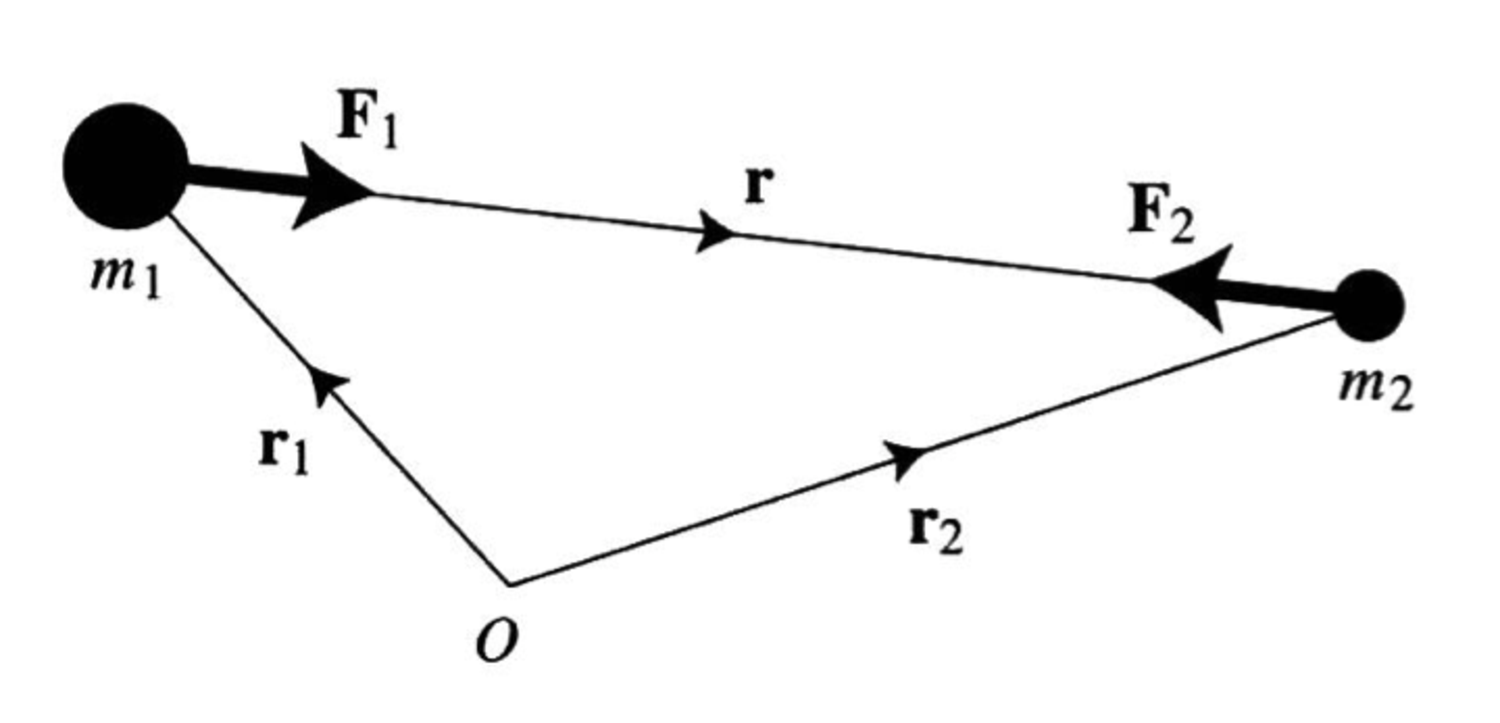
\includegraphics[width=10cm]{./image/sec2_1.pdf}
\caption{\label{fig:A}}
\end{figure}

(\ref{eq:mr}) 式を両辺2階積分する.
\begin{equation}
m_1 \dot{{\bm r}}_1 + m_2 \dot{{\bm r}}_2 = {\bm a} \quad {\rm and} \quad m_1 {\bm r}_1 + m_2 {\bm r}_2 = {\bm a} t + {\bm b}.
\end{equation}
${\bm a}, {\bm b}$ は定数ベクトル.${\bm R} = (m_1 {\bm r}_1 + m_2 {\bm r}_2)/(m_1 + m_2)$ を使って重心の位置ベクトルを表現する.
\begin{equation}
\dot{{\bm R}} = \frac{{\bm a}}{m_1 + m_2} \quad {\rm and} \quad {\bm R} = \frac{{\bm a} t + {\bm b}}{m_1 + m_2}.
\end{equation}
この式から,2体が互いの重力のみで運動している場合,その重心の運動は静止しているか,等速直線運動を行っているかのどちらかということになる.ここで,相対ベクトル ${\bm r}$ を使って運動方程式を書き直す.$\ddot{{\bm r}} = \ddot{{\bm r}}_2 - \ddot{{\bm r}}_1$ とすると (\ref{eq:F}) 式は,
\begin{equation}
\frac{d^2 {\bm r}}{dt^2} + \mu \frac{{\bm r}}{r^3} = 0. \label{eq:raletive}
\end{equation}
($\mu = G (m_1 + M_2)$) となり,相対運動の方程式となる.この方程式を解き $m_2$ の $m_1$ に対する相対軌道を得るためには,相対運動におけるいくつかの定数を求める必要がある. ここではまずそれらの運動の定数の一つである角運動量ベクトルについて述べる.

(\ref{eq:raletive}) 式の両辺と ${\bm r}$ の外積をとると,${\bm r} \times \ddot{{\bm r}} = 0$.さらに両辺積分すると,
\begin{equation}
{\bm r} \times \dot{{\bm r}} = {\bm h} \label{eq:angmom}
\end{equation}
${\bm h}$ は角運動量ベクトルであり,${\bm r}, \dot{{\bm r}}$ に垂直である定数ベクトルである.つまり,$m_2$ の相対運動は,${\bm r}, \dot{{\bm r}}$ に垂直な平面内に限定されることがわかる.この平面を軌道平面という.$m_2 \ll m_1$ とすれば $h = |{\bm h}|$ は単位質量あたりの $m_2$ の角運動量として近似できる.

ここで,${\bm r}$ を極座標で表現してみよう.座標原点は $m_1$ とし,$\theta = 0$ となる基準線は任意の位置でとることとする.また $m_1, m_2$ の重心は慣性系を運動しているが,$\theta = 0$ の基準線の方向は一定とする.動径方向の単位ベクトルを $\hat{{\bm r}}$,角度方向の単位ベクトルを $\hat{{\bm \theta}}$ として,位置,速度,加速度を表現すると以下のようになる.
\begin{equation}
{\bm r} = r \hat{{\bm r}}, \quad \dot{{\bm r}} = \dot{r} \hat{{\bm r}} + r \dot{\theta} \hat{{\bm \theta}}, \quad \ddot{{\bm r}} = (\ddot{r} - r \dot{\theta}^2) \hat{{\bm r}} + \left[ \frac{1}{r} \frac{d}{dt} (r^2 \dot{\theta})\right] \hat{{\bm \theta}}. \label{eq:polar}
\end{equation}

(\ref{eq:angmom}) 式に上記の ${\bm r}, \dot{{\bm r}}$ を代入すると,${\bm h} = r^2 \dot{\theta} \hat{{\bm z}}$ となる.$\hat{{\bm z}}$ は軌道平面に垂直な単位ベクトルであり,向きは ${\bm r}$ から ${\bm \theta}$ へ右ねじを回したときに進む方向である.これより,
\begin{equation}
h = r^2 \dot{\theta}.
\end{equation}
この式からわかることは以下の通りである.

質点 $m_2$ が微小時間 $\delta t$ の間だけ運動したとする.$t = 0$ のとき $m_2$ の座標が ($r, \theta$) とすれば,$t = \delta t$ の座標は ($r + \delta r, \theta + \delta \theta$) である.その間に動径ベクトルが横切る領域の面積は,
\begin{equation}
\delta A \approx \frac{1}{2} r (r + \delta r) \sin (\delta \theta) \approx \frac{1}{2} r^2 \delta \theta. 
\end{equation}
両辺を $\delta t$ で割り,$\delta t \rightarrow 0$ の極限をとると,
\begin{equation}
\frac{dA}{dt} = \frac{1}{2} r^2 \frac{d \theta}{dt} = \frac{1}{2} r^2 \dot{\theta} = \frac{1}{2} h. \label{eq:kepler2}
\end{equation}
$h$ は定数であるので,動径が一定時間に横切る軌道面の面積は常に一定であることがわかる.つまり (\ref{eq:kepler2}) は Kepler の第2法則 と等価である.しかし,このことは万有引力に対してのみ成り立つ訳ではなく,2物体の間に引力が働いていれば成り立つ.

\subsection{軌道と速度 \label{sec:position&velocity}}
(\ref{eq:polar}) 式の $\ddot{{\bm r}}$ を (\ref{eq:raletive}) 式に代入することで,相対運動のスカラー方程式を求めることができる.$r$ 成分を比べると,
\begin{equation}
\ddot{r} - r \dot{\theta}^2 = - \frac{\mu}{r^2}. \label{eq:scalar}
\end{equation}
$\theta$ の関数としての $r$ の解を求めるため,$u = 1/r$ として代入し,定数 $h = r^2 \dot{\theta}$ を使って時間 $t$を消去する必要がある.$r$ を時間微分すると,
\begin{equation}
\dot{r} = - \frac{1}{u^2} \frac{du}{d \theta} \dot{\theta} \quad {\rm and} \quad \ddot{r} = - h \frac{d^2 u}{d \theta^2} \dot{\theta} = - h^2 u^2 \frac{d^2 u}{d \theta^2}. 
\end{equation}
したがって (\ref{eq:scalar}) 式を書き換えると,
\begin{equation}
\frac{d^2 u}{d \theta^2} + u = \frac{\mu}{h^2}.
\end{equation}
この2階線形微分方程式の一般解は,
\begin{equation}
u =\frac{\mu}{h^2} \left[ 1+ e \cos (\theta - \varpi) \right].
\end{equation}
ここで振幅 $e$,位相 $\varpi$ は積分定数.よって $r$ は,
\begin{equation}
r =\frac{p}{1+ e \cos (\theta - \varpi)}.
\end{equation}
$p = h^2 / \mu$ は半直弦 ($\theta - \varpi = \pi / 2$ における $r$ の大きさ),$e$ は離心率と呼ばれる.この式は円錐曲線と呼ばれる.

円錐曲線から得られる曲線は $e$ によって区別され,4種類ある.
\begin{equation}
\begin{split}
円 &: \quad e = 0, \quad p = a; \\
楕円 &: \quad 0 < e < 1, \quad p = a(1-e^2); \\
放物線 &: \quad e = 1, \quad p = 2q; \\
双曲線 &: \quad e > 1, \quad p = a(e^2-1). 
\end{split}
\end{equation}
$a$ は軌道長半径.放物線の場合は $p$ を $q$ (放物線の近点距離) で定義する.

この2体問題の解から,太陽系の惑星の軌道は楕円の形をしており,閉じた軌道を描くと
考えられる.したがって Kepler の第1法則は逆2乗則の結果ととらえることができる.

\begin{figure}[H]
\centering
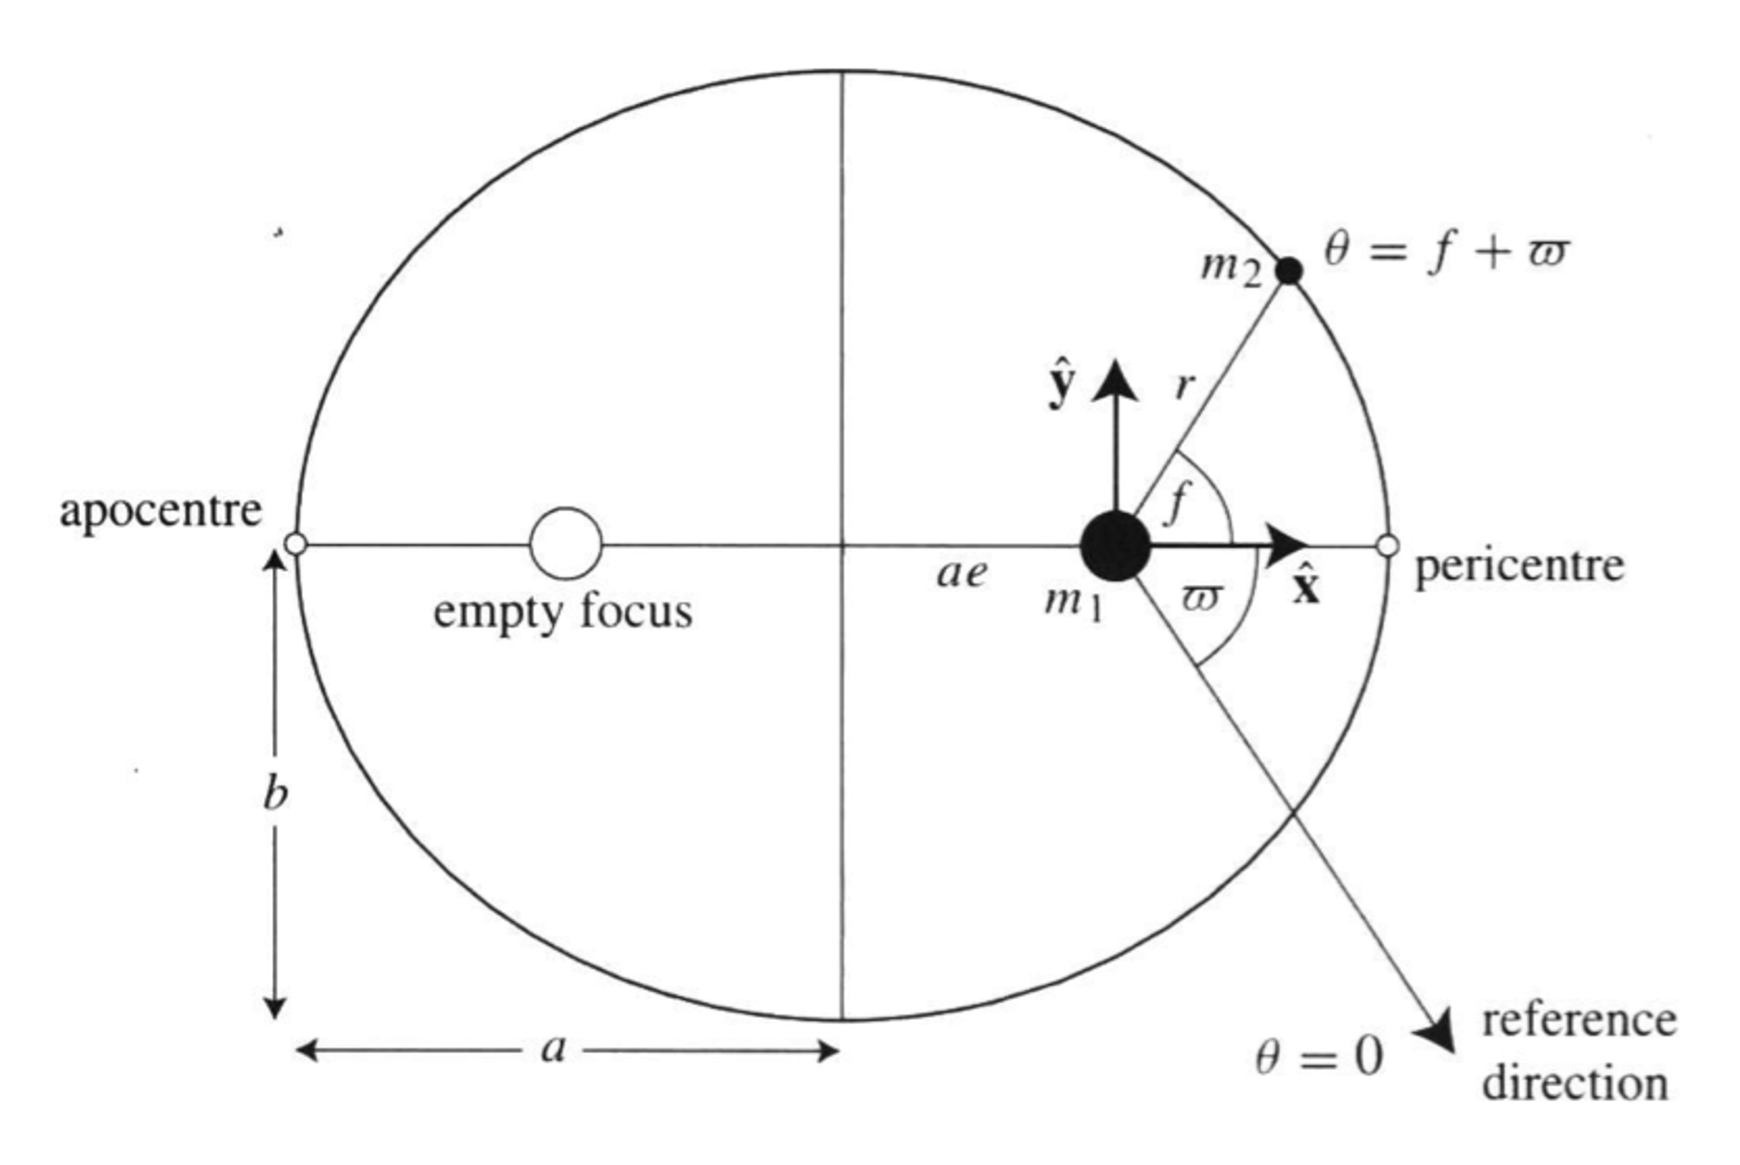
\includegraphics[width=10cm]{./image/sec2_5.pdf}
\caption{\label{fig:ellipse}}
\end{figure}

彗星はその多くが $e \approx 1$ の値を持つのに対して,冥王星 ($e = 0.25$),水星 ($e = 0.21$),そして海王星の衛星 Nereid ($e = 0.75$) という例外があるが,太陽系の主な天体のほとんどは $e \ll 1$ である.したがって,以下の議論では楕円運動に焦点を当てる.

楕円運動では $a, e$ には以下のような関係がある.
\begin{equation}
b^2 = a^2 (1 - e^2).
\end{equation}
ここで $b$ は軌道短半径である (図 \ref{fig:ellipse}).また $r$ は,
\begin{equation}
r =\frac{a (1 - e^2)}{1+ e \cos (\theta - \varpi)}.
\end{equation}
$\theta$ は黄経 (黄道座標の経度にあたり,春分点を0度としている) と呼ばれる.天体力学では,慣性系において固定された基準線からの角度を測るときに,慣習的に黄経を用いる.$\theta = \varpi, \theta = \varpi + \pi$ のときに,それぞれ $r$ の最小値 $r_{\rm p} = a (1 - e)$,最大値 $r_{\rm a} = a (1 + e)$ をとる.これらの点はそれぞれ近点,遠点と呼ばれる.楕円の中心からどちらかの焦点までの距離は $a e$ で与えられる.$\varpi$ ("curly pi" と発音) は近日点経度と呼ばれ,近点の黄経である.2体問題では $\varpi$ は定数であるが,他の摂動が入る場合は時間とともに変化する.大抵は黄経よりも $\varpi$ から測った角度の方がより扱いやすく,真近点離角 $f = \theta - \varpi$ を導入する.$f, \theta$ は $2 \pi$ の周期を持つ.よって $r$ は,
\begin{equation}
r = \frac{a (1 - e^2)}{1+ e \cos f}. \label{eq:rf}
\end{equation}
ここで,$m_1$ を中心として近点方向に $x$ 軸をとる直交座標を考えると,位置ベクトルの成分は,
\begin{equation}
x = r \cos f \quad {\rm and} \quad y = r \sin f. \label{eq:xy}
\end{equation}

ある軌道周期 $T$ で楕円上を一周するときに位置ベクトルが横切る面積は単純に $A = \pi a b$ である.(\ref{eq:kepler2}) 式よりこの面積は $h T / 2$ と等しい.ゆえに $h^2 = \mu p = \mu a (1 - e^2)$ より,
\begin{equation}
T^2 = \frac{4 \pi^2}{\mu} a^3. \label{eq:kepler3}
\end{equation}
これは Kepler の第3法則と等価である.この式から軌道周期 $T$ は離心率 $e$ に依存せず,軌道長半径 $a$ のみに依存することがわかる.

$\theta$ は 1周期につき $2 \pi$ だけ周期的に変化するため,平均運動 $n$ を次のように定義する.
\begin{equation}
n = \frac{2 \pi}{T}. \label{eq:n}
\end{equation}
さらに,(\ref{eq:kepler3}) 式より,
\begin{equation}
\mu = n^2 a^3 \quad {\rm and} \quad h = n a^2 \sqrt{1 - e^2} = \sqrt{\mu a (1 - e^2)}. \label{eq:mu}
\end{equation}
平均運動の値は2体問題では定数であるが,実際の角速度 $\dot{f}$ は経度の関数である.

運動に関するもう一つの定数を導出するため,$\dot{{\bm r}}$ と (\ref{eq:raletive}) 式の内積をとり,(\ref{eq:polar}) 式の ${\bm r}, \ddot{{\bm r}}$ の値を代入すると,
\begin{equation}
{\bm r} \cdot \ddot{{\bm r}} + \mu \frac{\dot{{\bm r}}}{r^2} = 0.
\end{equation}
これを両辺 $t$ で積分すると,
\begin{equation}
\frac{1}{2} v^2 - \frac{\mu}{r} = C. \label{eq:energyC}
\end{equation}
ここで $v^2 = \dot{{\bm r}} \cdot \dot{{\bm r}}$ は速度の2乗,$C$ は積分定数である.
(\ref{eq:energyC}) 式はエネルギー積分とも呼ばれ,単位質量あたりの天体のエネルギーが保存することを示している.ここまでの結果より,2体問題には4つの定数が保存する : エネルギー積分 $C$ と角運動量 ${\bm h}$ の3成分である.\ref{sec:elements} 節で導出するが,これらは軌道要素や離心率ベクトルのような別の量で表現することもできる.

$v^2$ の別の表式を見つけ, $C$ の別の表式を導出する.$\varpi$ は固定されているので,$\dot{\theta} = d (f + \varpi) / dt = \dot{f}$ であり,(\ref{eq:polar}) 式の ${\bm r}$ の定義を用いると,
\begin{equation}
v^2 = \dot{{\bm r}} \cdot \dot{{\bm r}} = \dot{r}^2 + r^2 \dot{f}^2. \label{eq:v2}
\end{equation}
(\ref{eq:rf}) 式を微分すると,
\begin{equation}
\dot{r} = \frac{r \dot{f} e \sin f}{1+ e \cos f}.
\end{equation}
$r^2 \dot{f} = h = n a^2 \sqrt{1 - e^2}$ を使うと,
\begin{eqnarray}
\dot{r} & = & \frac{n a}{\sqrt{1 - e^2}} e \sin f, \label{eq:rdot} \\
r \dot{f} & = & \frac{n a}{\sqrt{1 - e^2}} (1+ e \cos f). \label{eq:rfdot}
\end{eqnarray}
この2つの式から (\ref{eq:v2}) 式を書き換えると,
\begin{equation}
v^2 = \frac{n a^2}{1 - e^2} (1 + 2 e \cos f + e^2) = \frac{n a^2}{1 - e^2} \left( \frac{2 a (1 - e^2)}{r} - (1 - e^2) \right).
\end{equation}
したがって,
\begin{equation}
v^2 = \mu \left( \frac{2}{r} - \frac{1}{a} \right). \label{eq:v2new}
\end{equation}
この式から,天体の速度は近点 ($f = 0$) で最大値,遠点 ($f = \pi$) で最小値をとる.それぞれの値は,
\begin{equation}
v_{\rm p} = n a \sqrt{\frac{1 + e}{1 - e}} \quad {\rm and} \quad v_{\rm a} = n a \sqrt{\frac{1 - e}{1 + e}}.
\end{equation}

また,(\ref{eq:xy}) 式をそれぞれ時間微分し,(\ref{eq:rdot}),  (\ref{eq:rfdot}) 式を代入して,速度の $x, y$ 成分を求めると,
\begin{equation}
\dot{x} = - \frac{n a}{\sqrt{1 - e^2}} \sin f \quad {\rm and} \quad  \dot{y} = + \frac{n a}{\sqrt{1 - e^2}} (e^2 + \cos f). \label{eq:xdotydot}
\end{equation}

(\ref{eq:v2new}) 式と (\ref{eq:energyC}) 式を比較すると,エネルギー積分 C は以下の形で表される.
\begin{equation}
C = - \frac{\mu}{2 a}. \label{eq:C}
\end{equation}
したがって,楕円軌道のエネルギーは軌道長半径のみの関数であり,離心率には依存しない.放物線軌道と双曲線軌道のエネルギーも同様に示すことができる.
\begin{equation}
C_{{\rm para}} = 0, \quad {\rm and} \quad C_{{\rm hyper}} = \frac{\mu}{2 a}.
\end{equation}

\subsection{平均近点離角と離心近点離角}
前節において,軌道長半径と離心率がわかっている場合に,真近点離角 $f$ が与えられれば,軌道の距離と速度を計算できることを示した.しかし,通常は任意の時間での天体の位置を計算したいと考えるのが普通である.$f$ と $r$ は $t$ の関数であるが,前節では依存性を示していない.

$2 \pi$ 周期かつ時間に関して線形な関数である角度を導入する.この角度は,後にさまざまな量の時間平均を計算するときに特に有益となる.(\ref{eq:n}) 式の平均運動 $n$ の定義を用いて,平均近点離角 $M$ を定義する.
\begin{equation}
M = n (t - \tau). \label{eq:M}
\end{equation}
ここで,$\tau$ は近点通過時刻.$M$ は角度の次元であり,平均運動と等しい一定の割合で線形的に増加するが,幾何学的に意味のある値ではない.しかし,$M$ の定義と (\ref{eq:rf}) 式から,$t = \tau$ (近点を通過) や $t = \tau + T / 2$ (遠点を通過) のとき,それぞれ $M = f =0, M = f = \pi$ となることは明らかである.$t$ が周期の整数倍のときも同様の関係を持つ.

$M$ は幾何学的に意味のある値ではないが,ある角度と関係がある.半径 $a$ の円を,軌道長半径 $a$,離心率 $e$ の楕円に外接させ (図 \ref{fig:Ef} (a)),その楕円のある点から長軸に垂直な直線を引き,外接円に交差させる. すると,$f = 0$ の基準線 (長軸) と,楕円の中心からその外接円上の交点までを結ぶ直線とのなす角で定義される,離心近点離角 $E$ という角度を決めることができる (図 \ref{fig:Ef} (b)).したがって,$E = 0$ は $f = 0$ と一致し,$E = \pi$ は $f = \pi$ と一致する.

\begin{figure}[H]
\centering
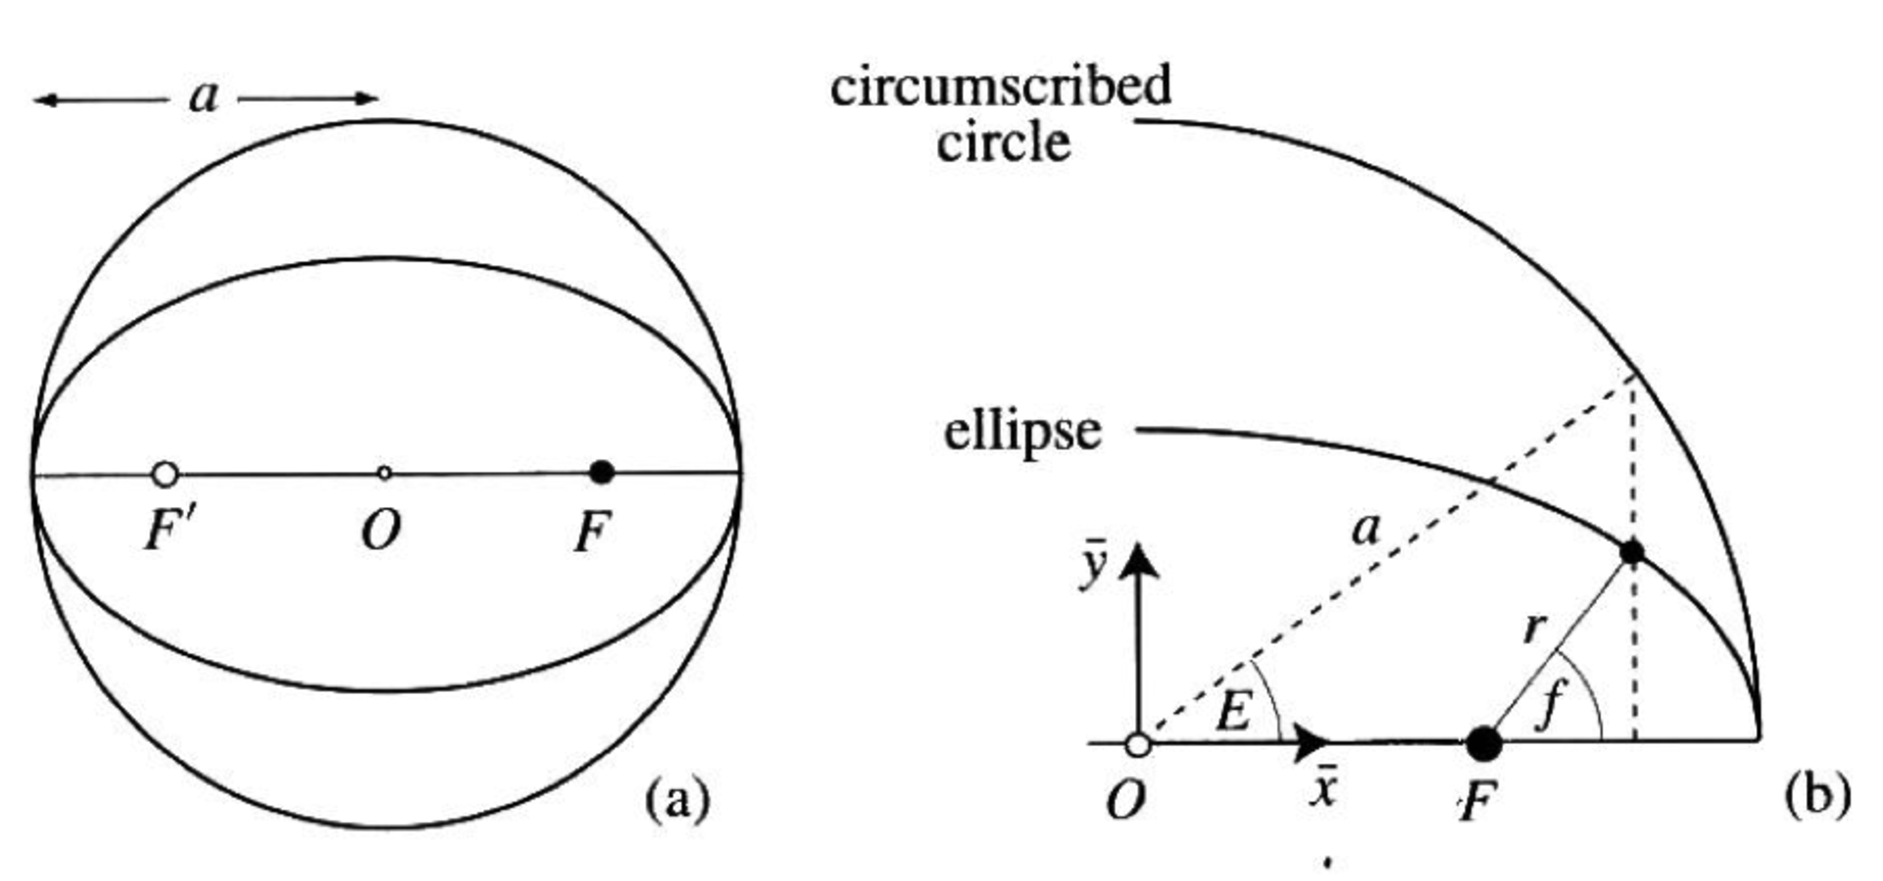
\includegraphics[width=10cm]{./image/sec2_7.pdf}
\caption{\label{fig:Ef}}
\end{figure}

図 \ref{fig:Ef} (b) 中の $\bar{x}, \bar{y}$ のように楕円中心を原点にとる直交座標系での楕円の方程式は,
\begin{equation}
\left( \frac{\bar{x}}{a} \right)^2 + \left( \frac{\bar{y}}{b} \right)^2 = 1.
\end{equation}
$\bar{x} = e \cos E$ から $\bar{y}^2 = b^2 \sin^2 E$ が求まり,$b^2 = a^2 (1 - e^2)$ の関係から $\bar{y} = a \sqrt{1 - e^2} \sin E$ が求まる.したがって外接円への $r$ の水平方向と垂直方向の射影は,$E$ を用いて表すと,
\begin{equation}
x = a (\cos E - e) \quad {\rm and} \quad y = a \sqrt{1 - e^2} \sin E. \label{eq:xEyE}
\end{equation}
これらの2乗和の平方根をとると,
\begin{eqnarray}
r & = & a (1 - e \cos E), \label{eq:rE} \\
\cos f & = & \frac{\cos E - e}{1 - e \cos E}. \label{eq:fE}
\end{eqnarray}
さらに,離心近点離角 $E$ と真近点離角 $f$ の関係のより簡単な表式が導出できる.
\begin{equation}
1 - \cos f = \frac{(1 + e) (1 - \cos E)}{1 - e \cos E}, \quad 1 + \cos f = \frac{(1 - e) (1 + \cos E)}{1 - e \cos E}.
\end{equation}
三角関数の2倍角の公式を使えば,
\begin{equation}
2 \sin^2 \frac{f}{2} = \frac{1 + e}{1 - e \cos E} 2 \sin^2 \frac{E}{2}, \quad 2 \cos^2 \frac{f}{2} = \frac{1 - e}{1 - e \cos E} 2 \cos^2 \frac{E}{2}.
\end{equation}
ゆえに,
\begin{equation}
\tan \frac{f}{2} = \sqrt{\frac{1 + e}{1 - e}} \tan \frac{E}{2}. \label{eq:fEnew}
\end{equation}
したがって,$E$ がわかっているとき,(\ref{eq:rE}) 式を使えば $r$ を,(\ref{eq:fE}) 式または (\ref{eq:fEnew}) 式を使えば $f$ を決定することができる.しかし,任意の時間 $t$ における天体の位置を知るには,$M$ と $E$ の関係を明らかにする必要がある.

$v^2 = \dot{r}^2 + (r \dot{f})^2$ と (\ref{eq:rfdot}), (\ref{eq:v2new}) 式を使うと,
\begin{eqnarray}
\dot{r}^2 & = & n^2 a^3 \left( \frac{2}{r} - \frac{1}{a} \right) - \frac{n^2 a^4 (1 - e^2)}{r^2}, \\
\frac{dr}{dt} & = & \frac{na}{r} \sqrt{a^2 e^2 - (r - a)^2}. \label{eq:drdt}
\end{eqnarray}
この式は (\ref{eq:rE}) 式を用いた以下の置き換えで積分可能となる.
\begin{equation}
r - a = - a e \cos E.
\end{equation}
よって (\ref{eq:drdt}) 式は,
\begin{equation}
\frac{dE}{dt} = \frac{n}{1 - e \cos E}. \label{eq:dEdt}
\end{equation}
この式は (\ref{eq:xEyE}) 式をそれぞれ時間微分し,${\bm r} \times \dot{{\bm r}} = h ( = n a^2 \sqrt{1 - e^2} )$ に代入することでも求めることができる.(\ref{eq:dEdt}) 式は簡単に積分できて,
\begin{equation}
n (t - \tau) = E - e \sin E. \label{eq:tauE}
\end{equation}
$t = \tau$ のとき $E = 0$.したがって(\ref{eq:M}) 式は,
\begin{equation}
M = E - e \sin E. \label{eq:keplereq}
\end{equation}
この式は Kepler 方程式と呼ばれ,その解は,任意の時間における軌道上の位置を求める際になくてはならないものである.ある時間が与えられたとき,(i) (\ref{eq:M}) 式から $M$ を求め,(ii) $E$ について (\ref{eq:keplereq}) 式を解き,(iii) (\ref{eq:xEyE}) 式または (\ref{eq:fE}) 式と,(\ref{eq:rf}) 式を使って$r, f$ を決める.

\subsection{軌道要素 \label{sec:elements}}
 \ref{sec:EoM} 節では,$m_1$ に対する $m_2$ の相対位置ベクトルと速度ベクトルが,常に角運動量ベクトルに垂直な平面上に存在することを示した.$m_2$ の ${\bm r} = (x, y)$ と $\dot{\bm r} = (\dot{x}, \dot{y})$ は3つの定数 $a, e, \varpi$ と変数 $f$ によって固有の値をもつ.ここまでの解析では軌道面上の運動を理解してきた.しかし,太陽系の天体の運動は単一の基準面上で起こるものではなく,ここからは軌道の3次元表現を考えていく (図 \ref{fig:elements_SSD}).
 
任意の位置が位置ベクトル ${\bm r} = (x, y, z) = x \hat{\bm x} + y \hat{\bm y} + z \hat{\bm z}$ で表現される3次元直交座標系を考える.3つの軸が右手系をなすように,$x$ 軸は楕円軌道の長軸上の近点の方向,$y$ 軸は 軌道面上の$x$ 軸に垂直な方向,そして $z$ 軸は $x, y$ 軸両方に垂直で $\hat{\bm x} \times \hat{\bm y}$ の方向にとる.

この軌道面から基準面を参照するために,基準面上の基準線の方向を $X$ 軸にとるような別の3次元直交座標系を考える.上と同様に3つの軸が右手系をなすように,$Y$  軸は基準面上の$X$ 軸に垂直な方向,そして $Z$ 軸は $X, Y$ 軸両方に垂直で $\hat{\bm X} \times \hat{\bm Y}$ の方向にとる.この座標系の例として,太陽のまわりを回る惑星の運動の場合,日心座標系 (太陽を中心とし,基準面を地球軌道面 (黄道面),基準線を地球の赤道面と黄道面の交線に沿った方向,すなわち春分の方向にとる座標系) が慣習的に使われる.注意すべきことは,他の天体による摂動を受けるため,特定の基準面を決めてもその基準面は時間変化してしまうことである.

\begin{figure}[H]
\centering
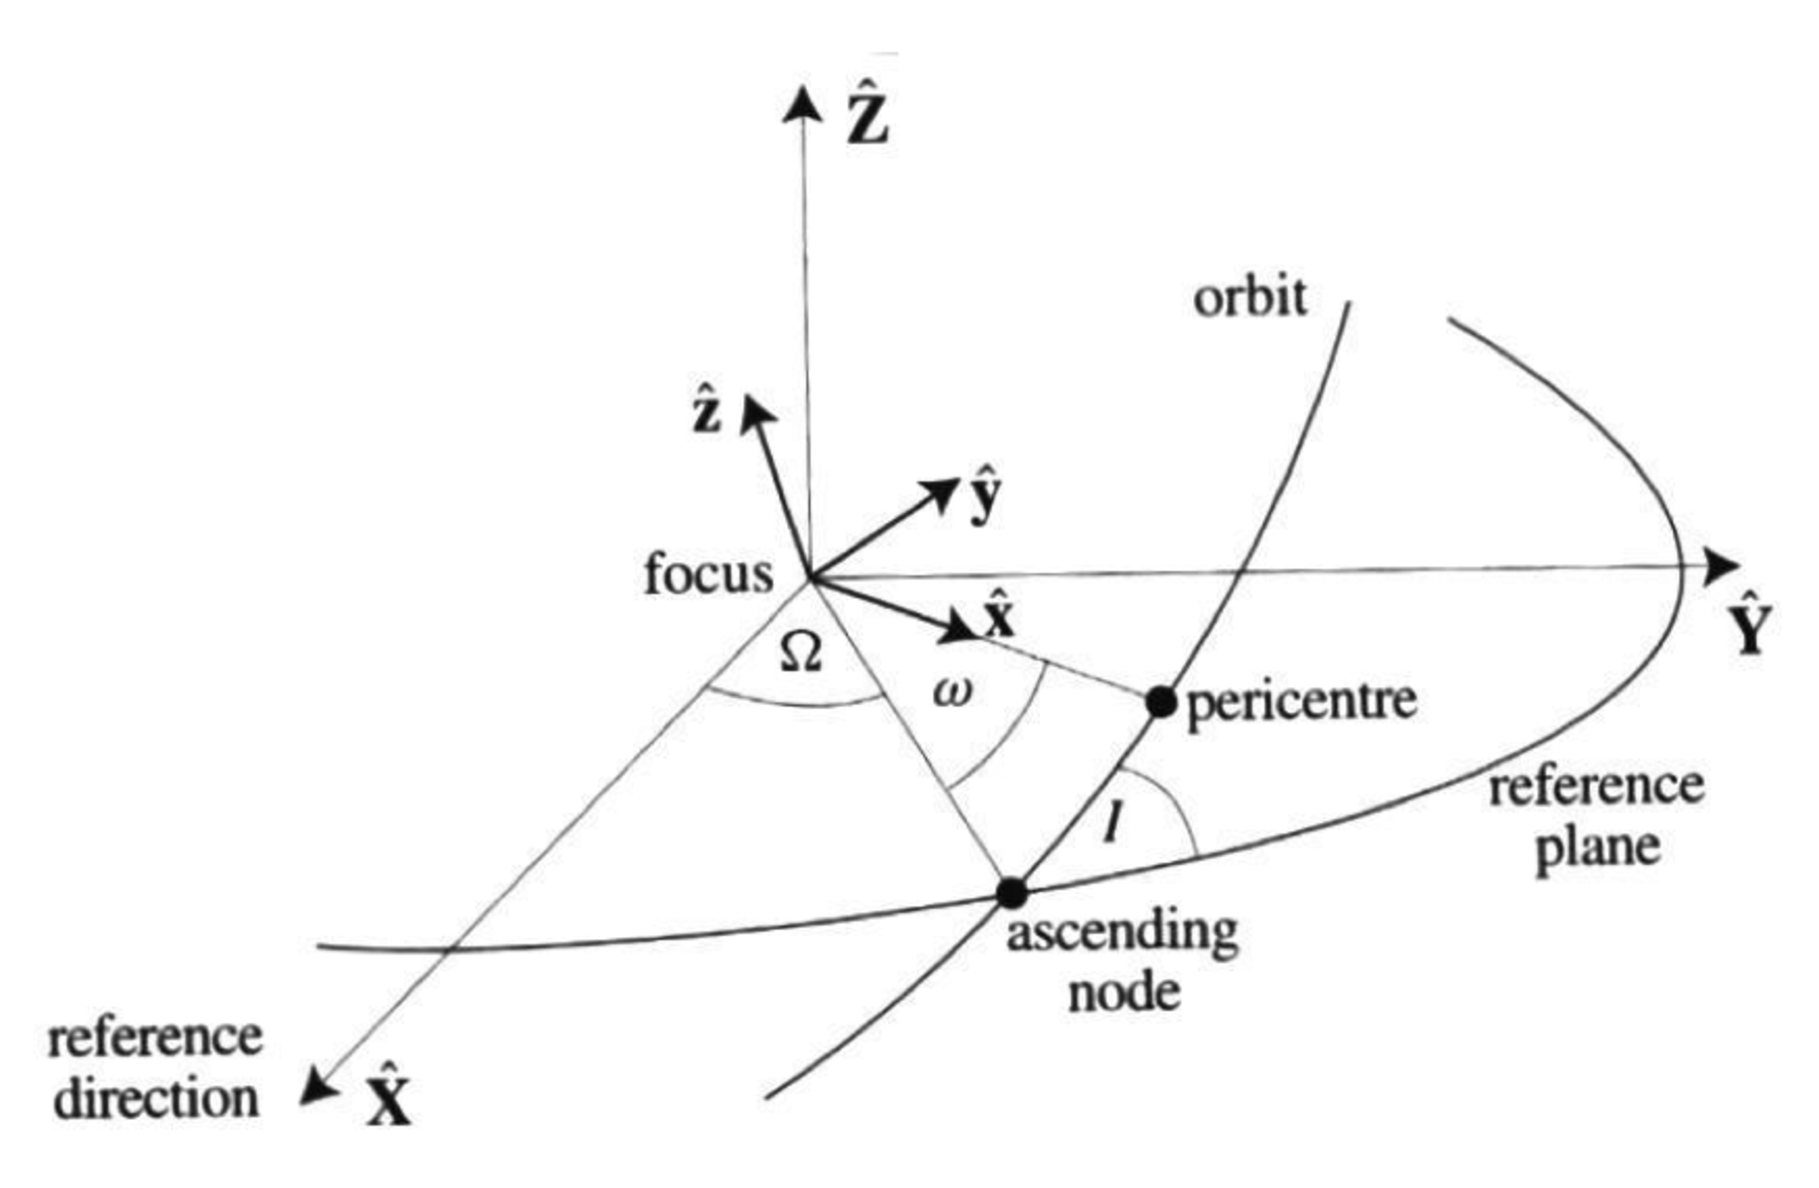
\includegraphics[width=10cm]{./image/sec2_13.pdf}
\caption{\label{fig:elements_SSD}}
\end{figure}

一般に軌道面は基準面に対して軌道傾斜角 (inclination,$I$) と呼ばれる角度だけ傾いている.軌道面と基準面が交わる線を交線 (line of nodes) と呼ぶ.基準面に対して下から上に軌道が横切る際の交点を昇交点 (ascending node),基準線と昇交点の動径ベクトルのなす角を昇交点経度 (longitude of ascending node,$\Omega$) と呼ぶ.昇交点の動径ベクトルと近点の方向のなす角を近日点引数 (argument of perisentre,$\omega$) と呼ぶ.

軌道傾斜角は常に $0 \leq I \leq 180^{\circ}$ である.$I \leq 90 ^{\circ}$ の場合は順行 (prograde),一方 $I \geq 90 ^{\circ}$ の場合は逆行 (retrograde) と呼ぶ.

$I \to 0$ の極限では軌道面は基準面と同一平面上に存在し,
\begin{equation}
\varpi = \Omega + \omega \label{eq:varpi}
\end{equation}
ここで $\varpi$ は \ref{sec:position&velocity} 節で導入した近日点経度である.しかし $\Omega$ と $\omega$ は異なる平面上で定義される角度にも関わらず, (\ref{eq:varpi}) の $\varpi$ の定義は軌道が傾いている場合にも使われる.ゆえに,$\varpi$ は一般に "曲がった" 角 ("dogleg" angle) とも呼ばれる.

図 \ref{fig:xyzXYZ} は軌道面の座標系と基準面の座標系の関係を示している.1つの座標系は,他の座標系を軸に沿って回転させることで表現できることがわかる.

軌道面の座標系 ($x, y, z$) から基準面の座標系 ($X, Y, Z$) へ変換するためには,(i) $x$ 軸が交線 (line of nodes) と一致するように $z$ 軸を中心に $\omega$ だけ回転させ,(ii) 次に2つの平面が一致するように $x$ 軸を中心に $I$ だけ回転させ,(iii) 最後に $z$ 軸を中心に $\Omega$ だけ回転させる (図 \ref{fig:elements_SSD},\ref{fig:xyzXYZ},\ref{fig:grapher} 参照).

\begin{figure}[H]
\centering
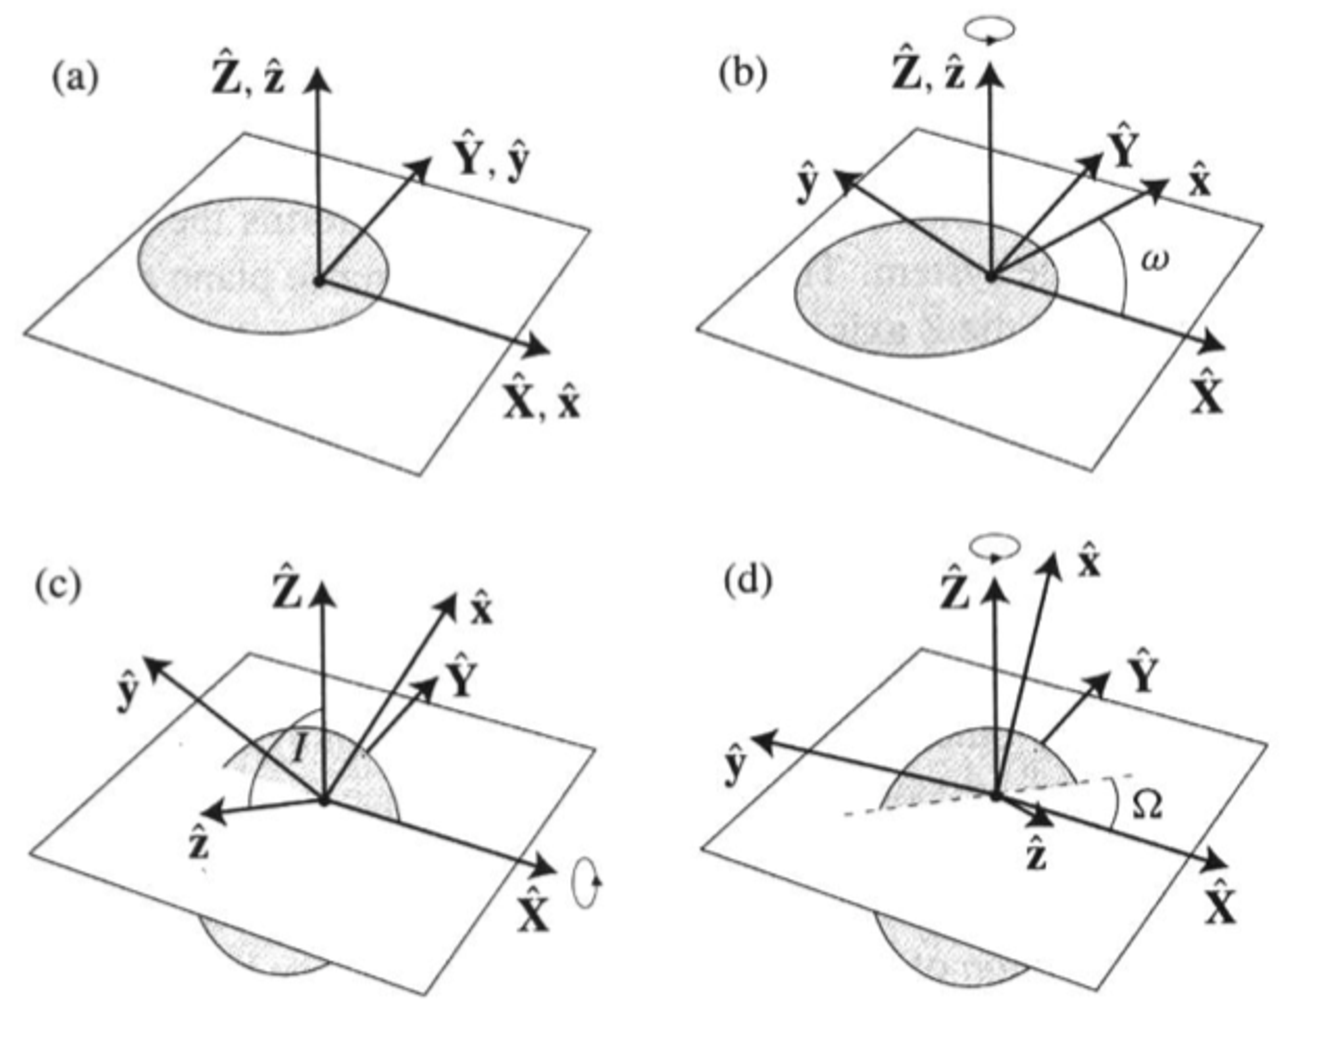
\includegraphics[width=10cm]{./image/sec2_14.pdf}
\caption{\label{fig:xyzXYZ}}
\end{figure}

\begin{figure}[H]
\begin{tabular}{cc}
%左
\begin{minipage}[t]{0.45\hsize}
\centering
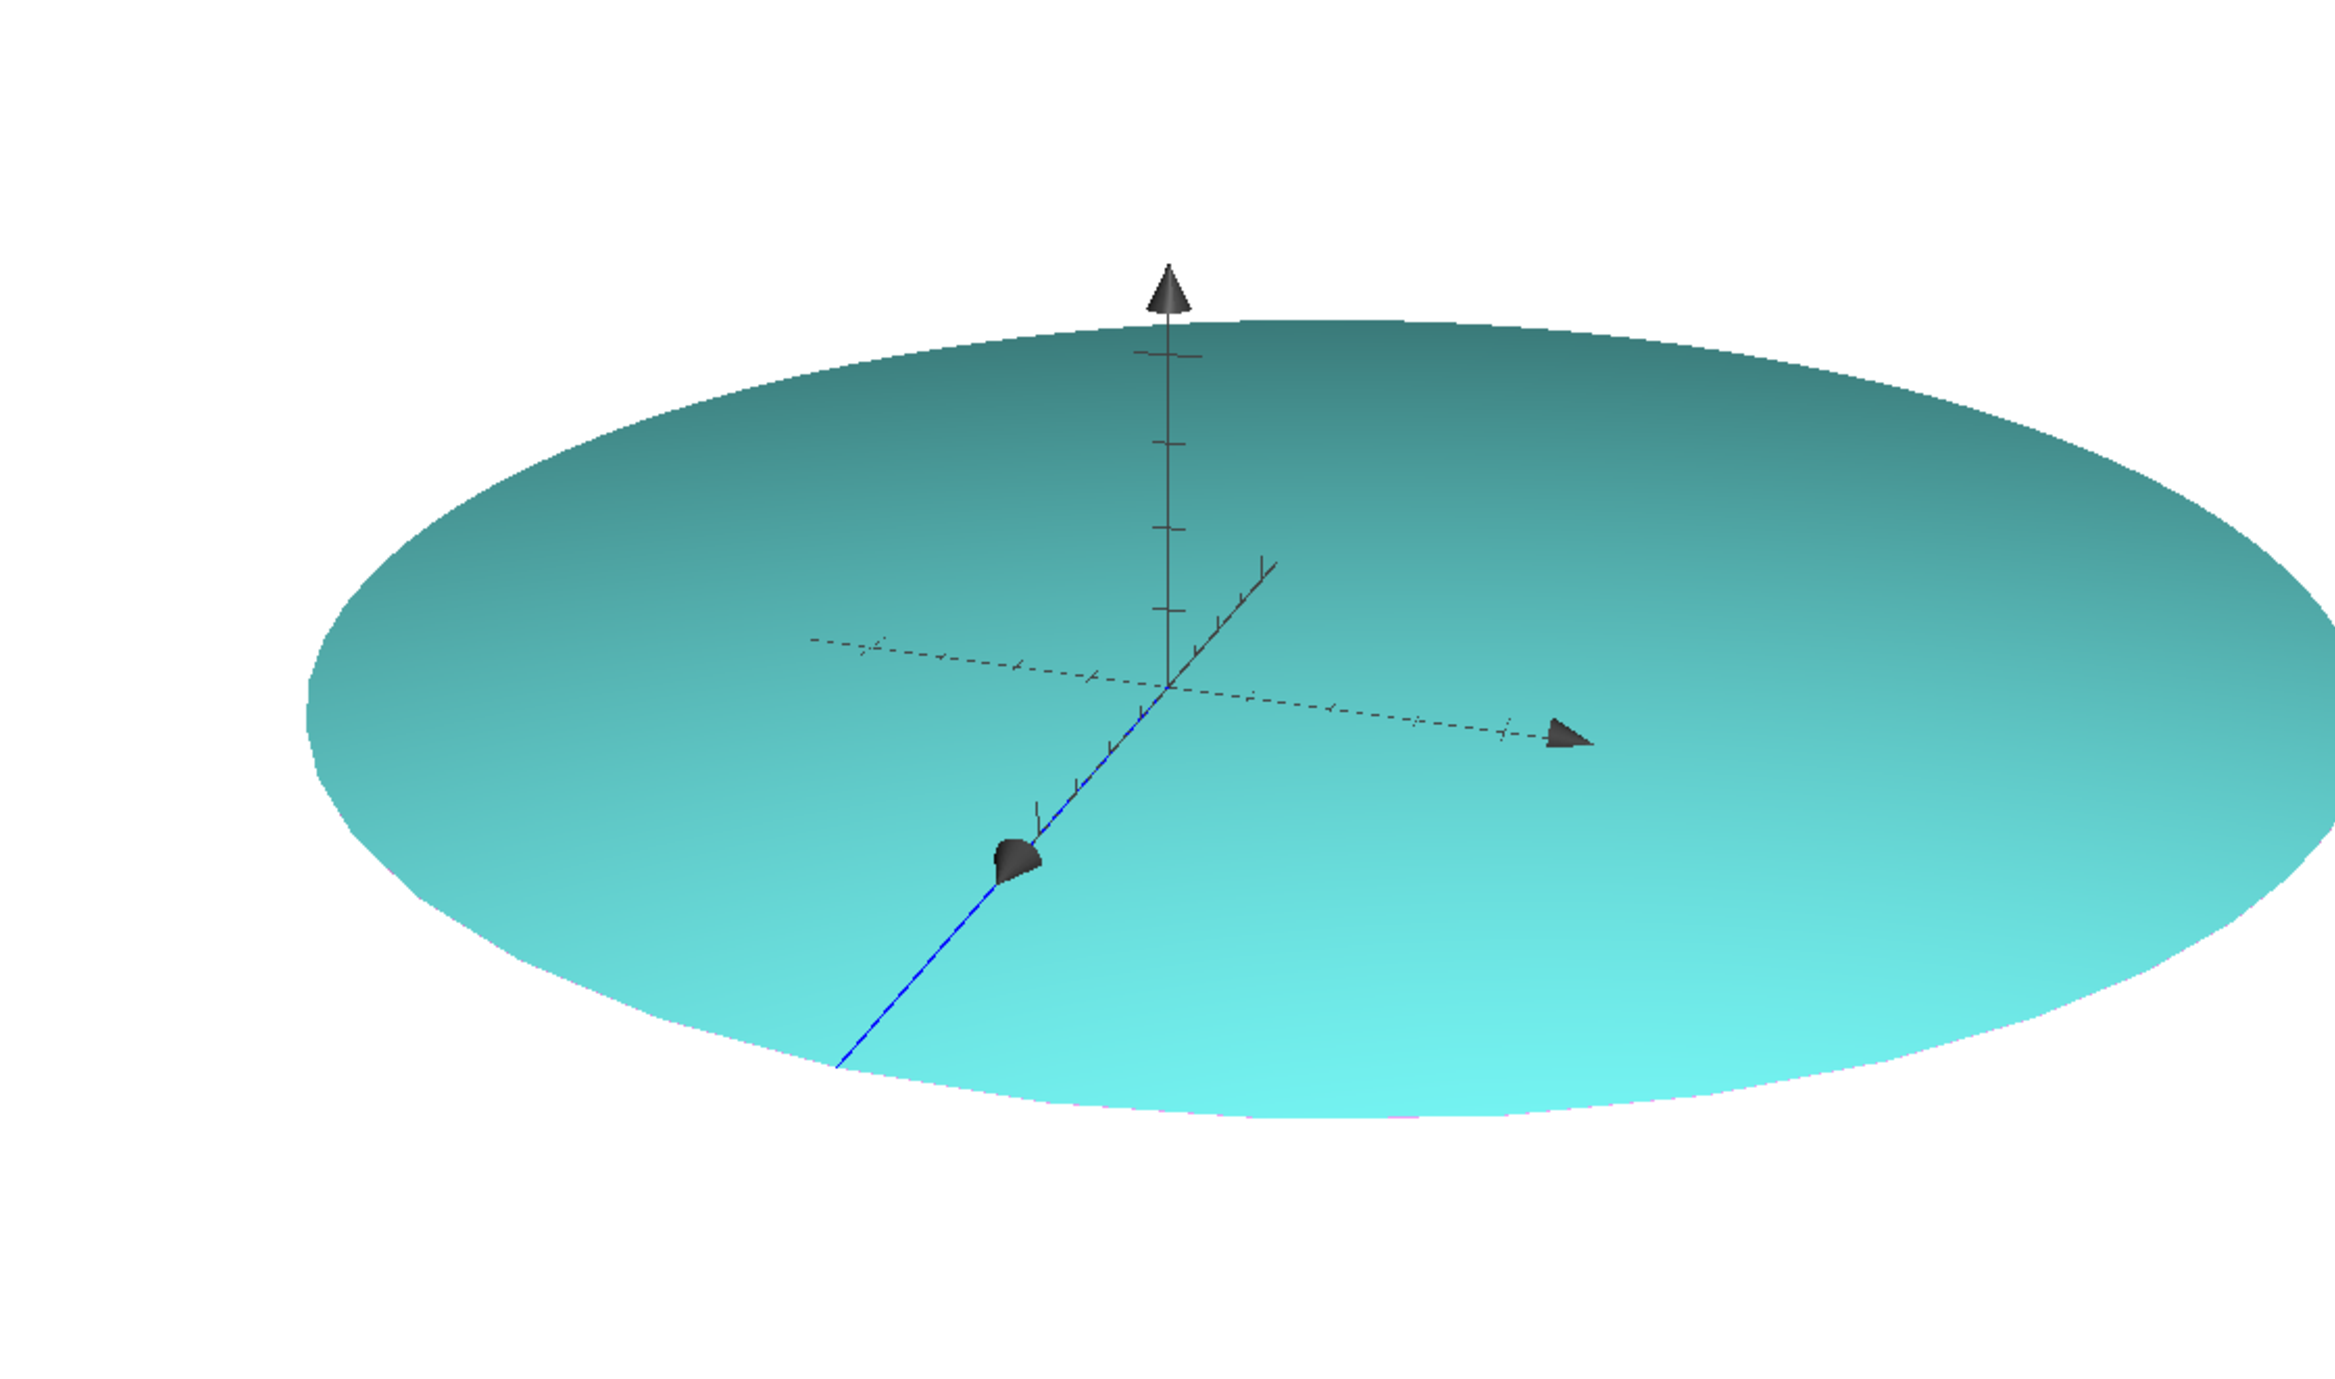
\includegraphics[width=7cm]{./image/ellipse1.pdf}
\end{minipage} &
%右
\begin{minipage}[t]{0.45\hsize}
\centering
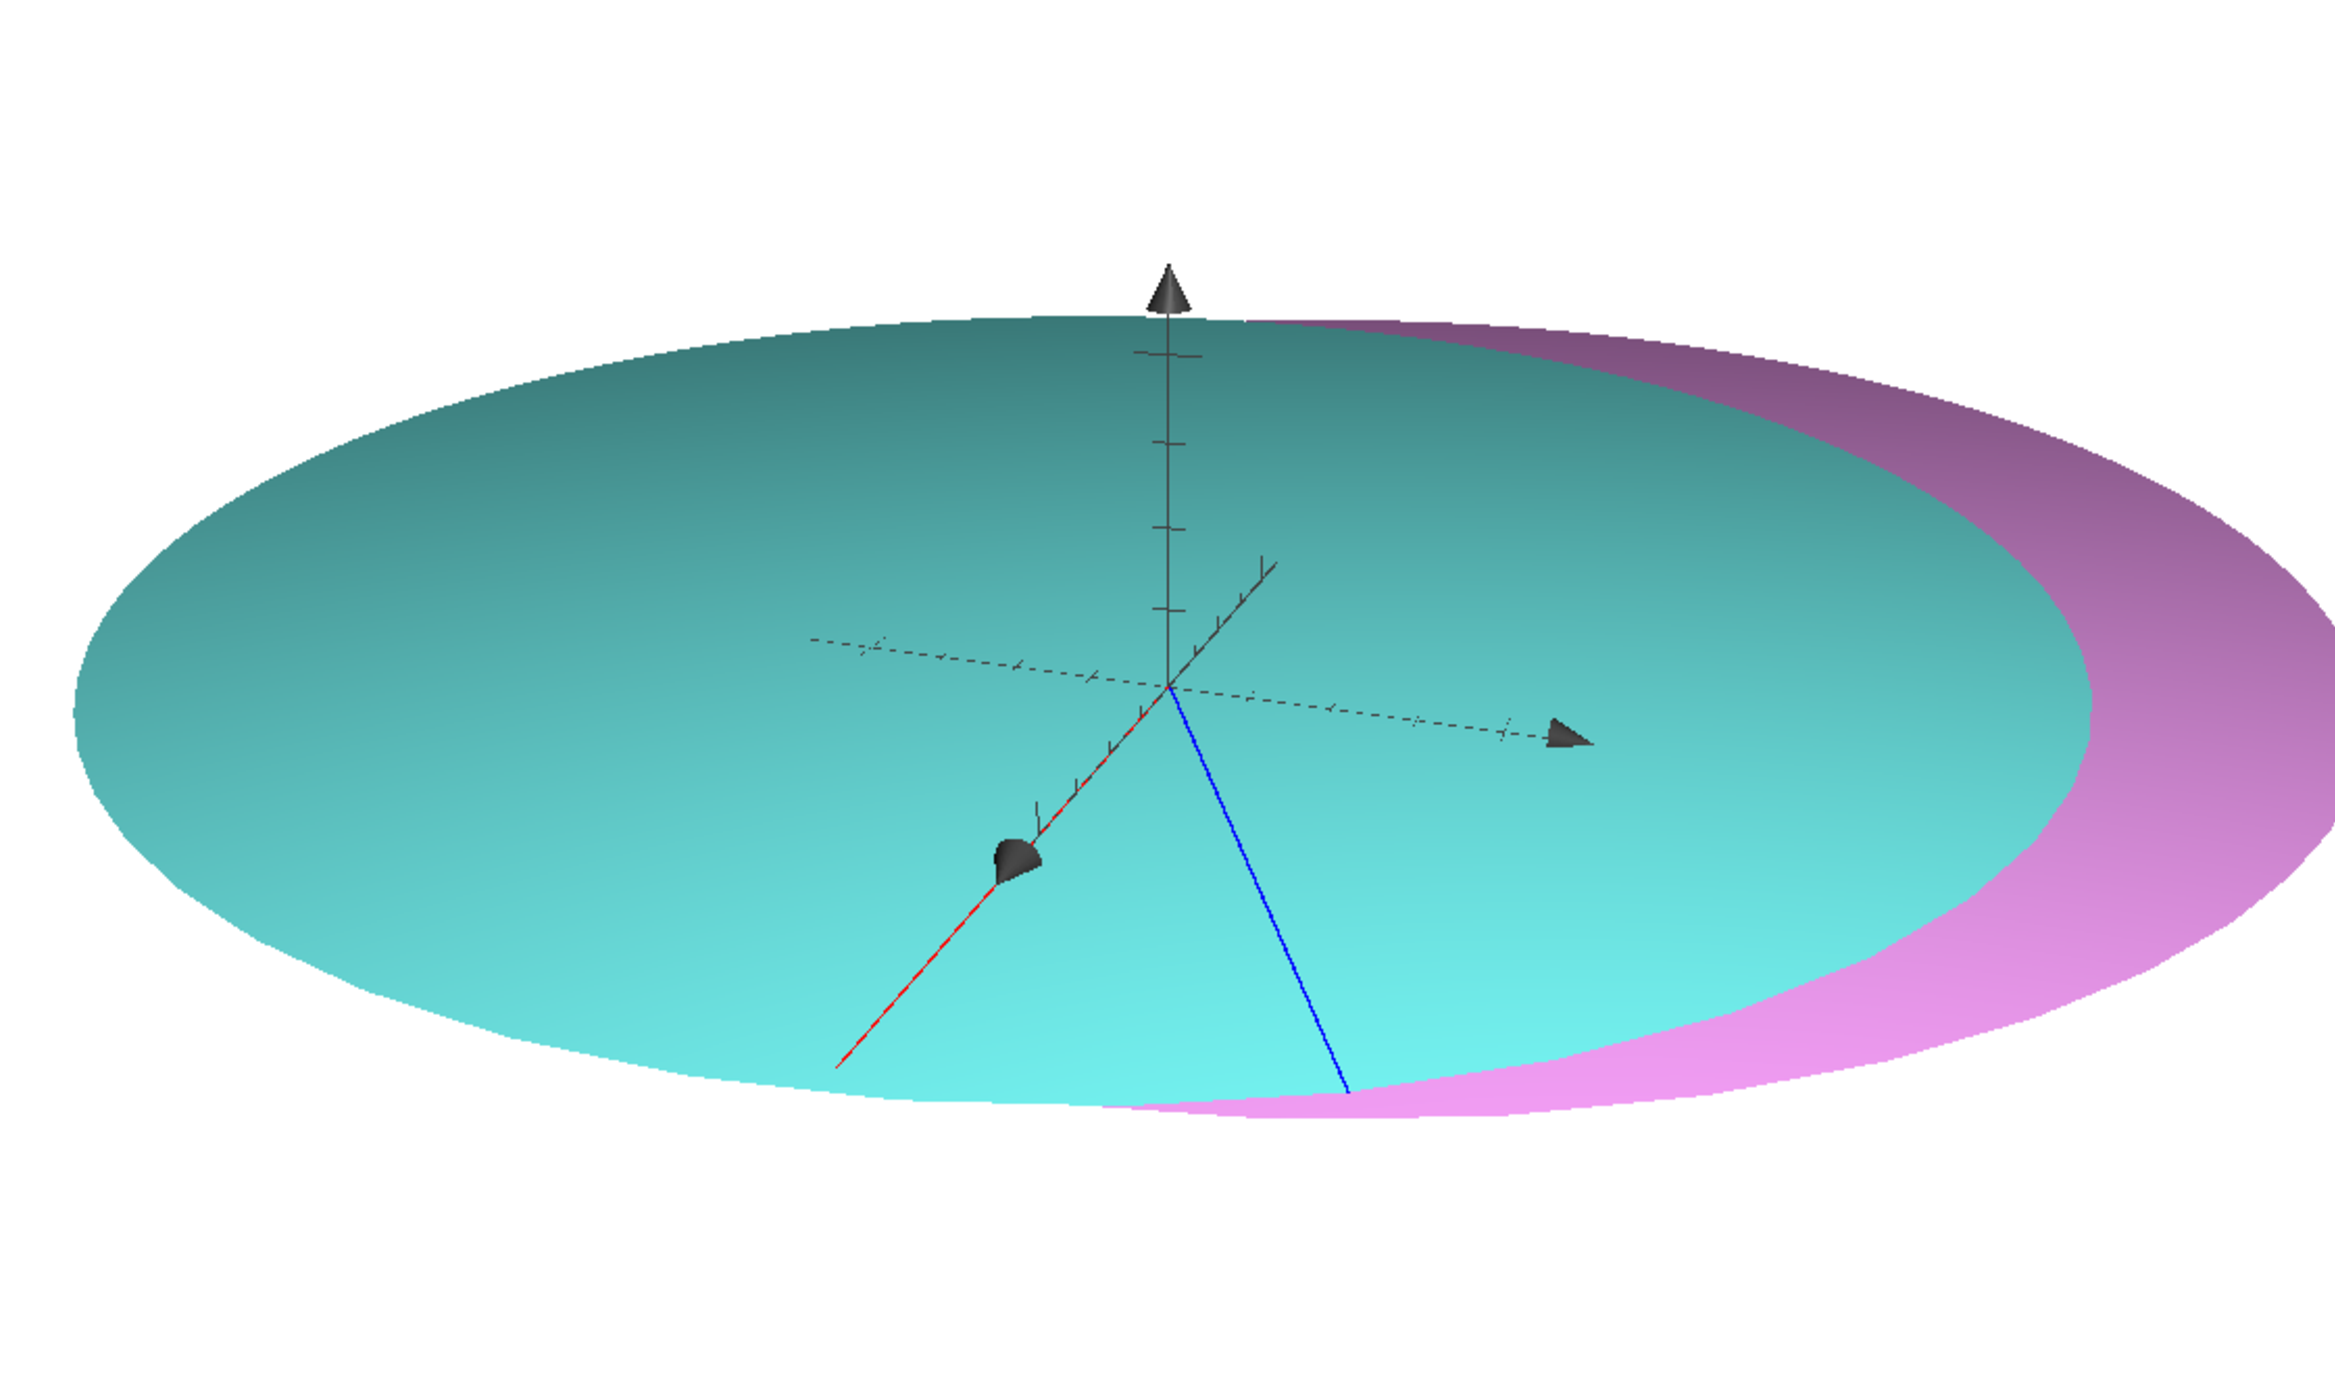
\includegraphics[width=7cm]{./image/ellipse2.pdf}
\end{minipage}\\
%
%左
\begin{minipage}[t]{0.45\hsize}
\centering
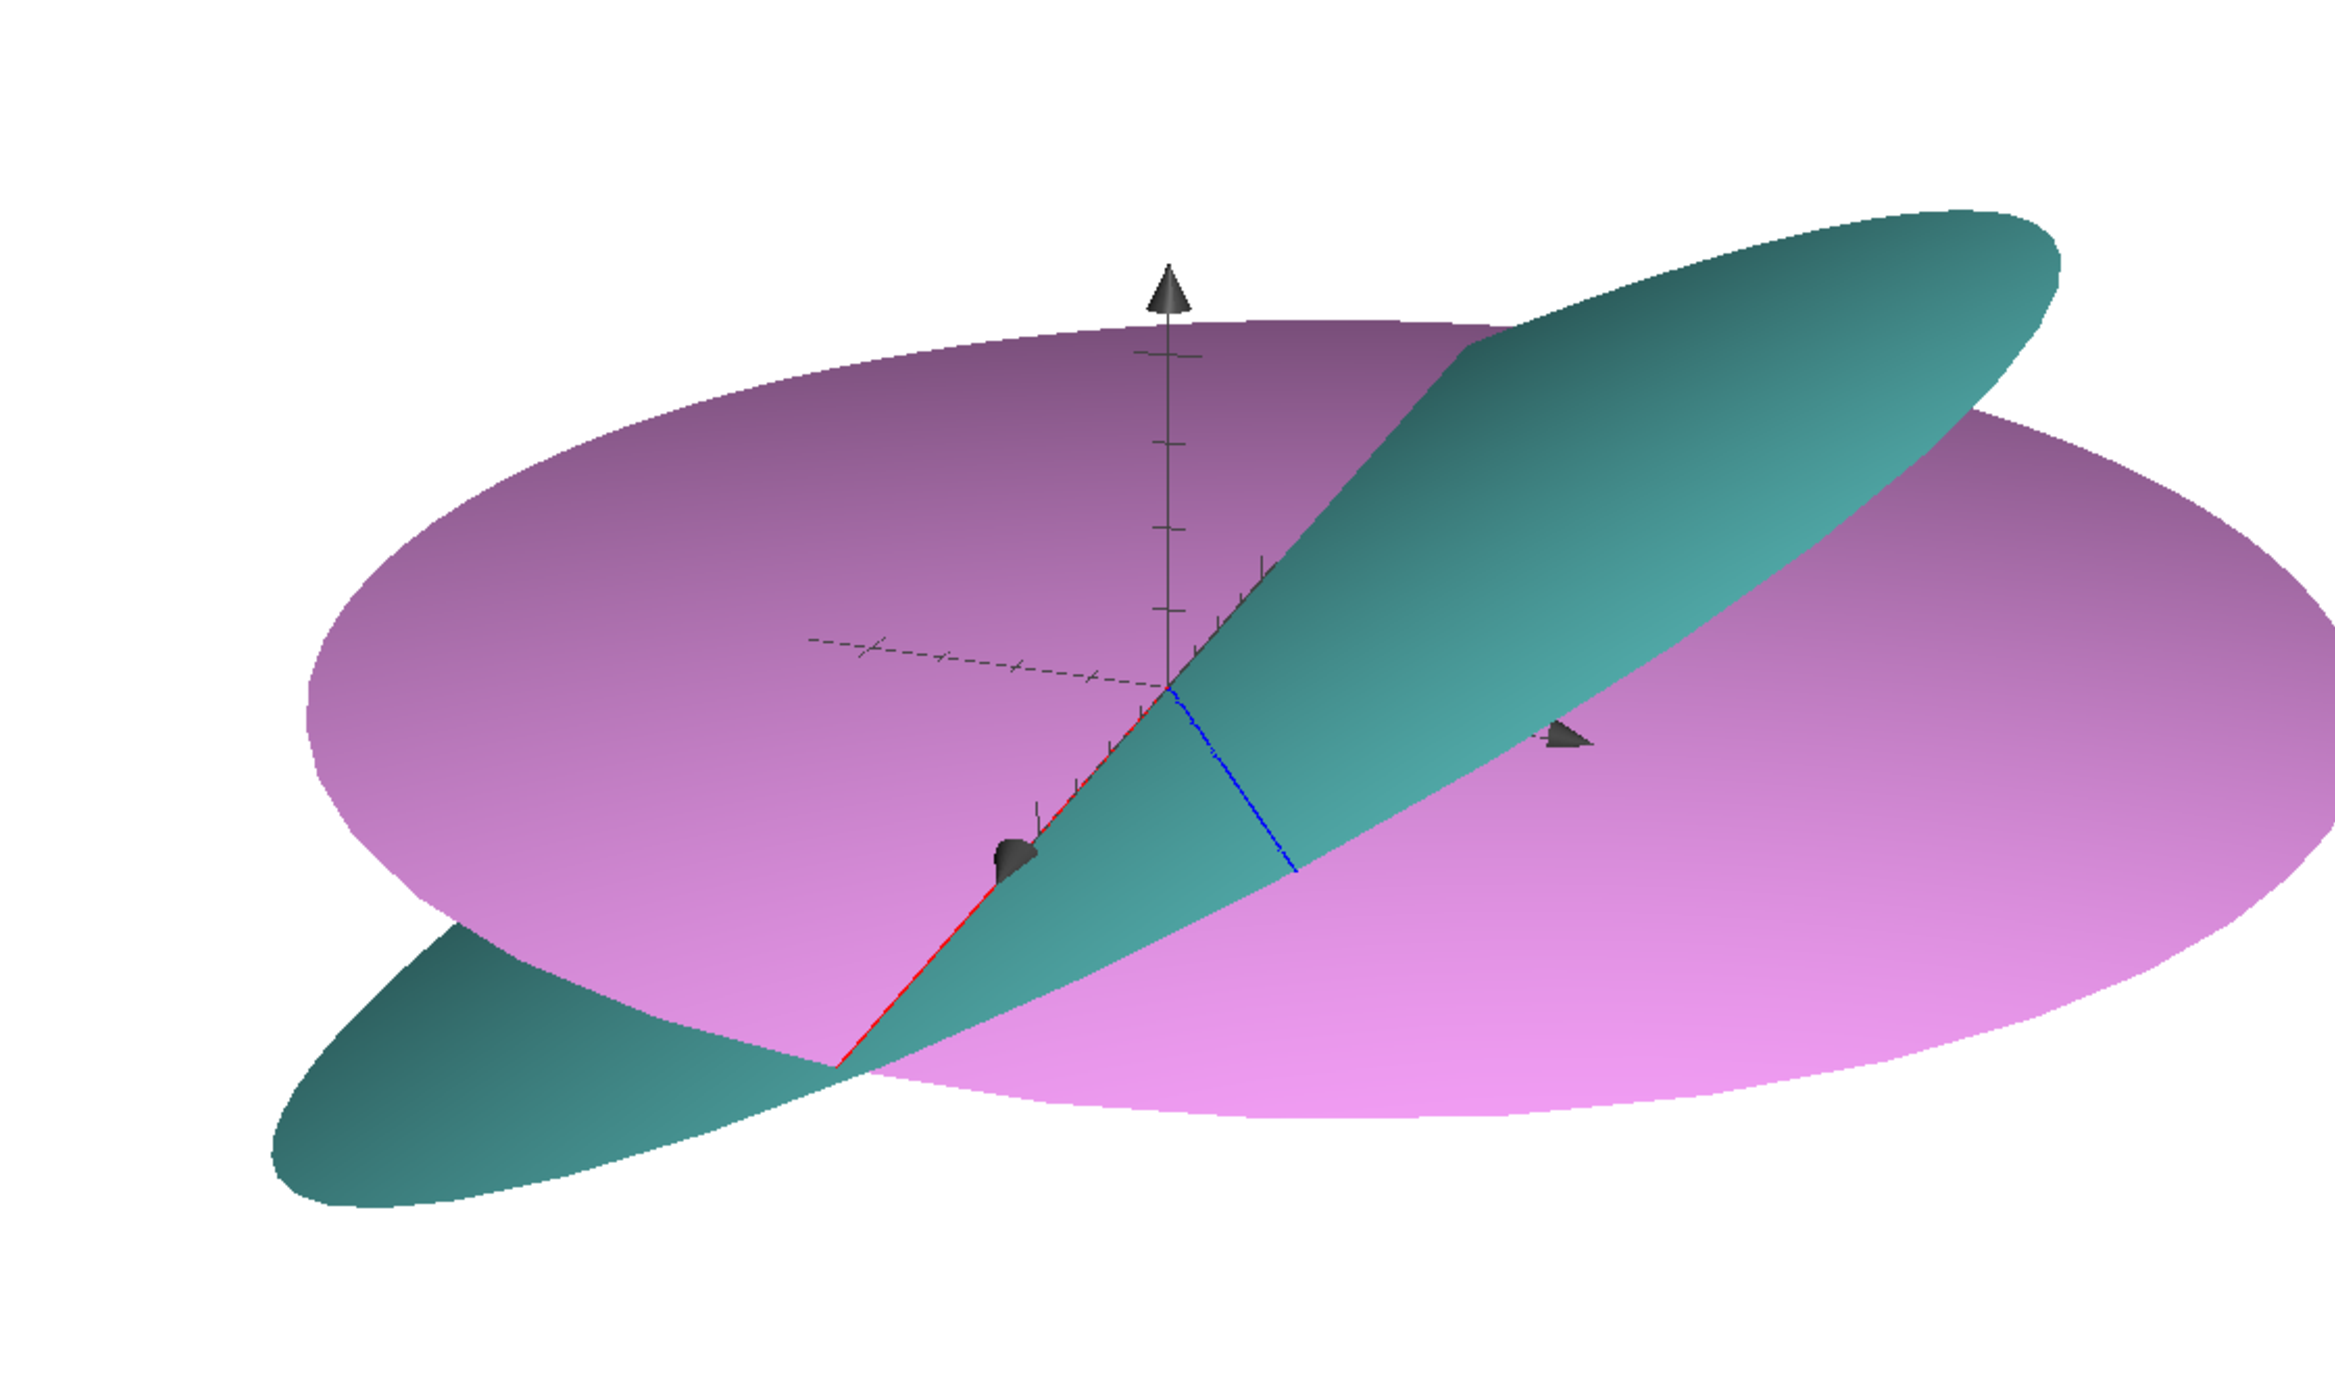
\includegraphics[width=7cm]{./image/ellipse3.pdf}
\end{minipage} &
%右
\begin{minipage}[t]{0.45\hsize}
\centering
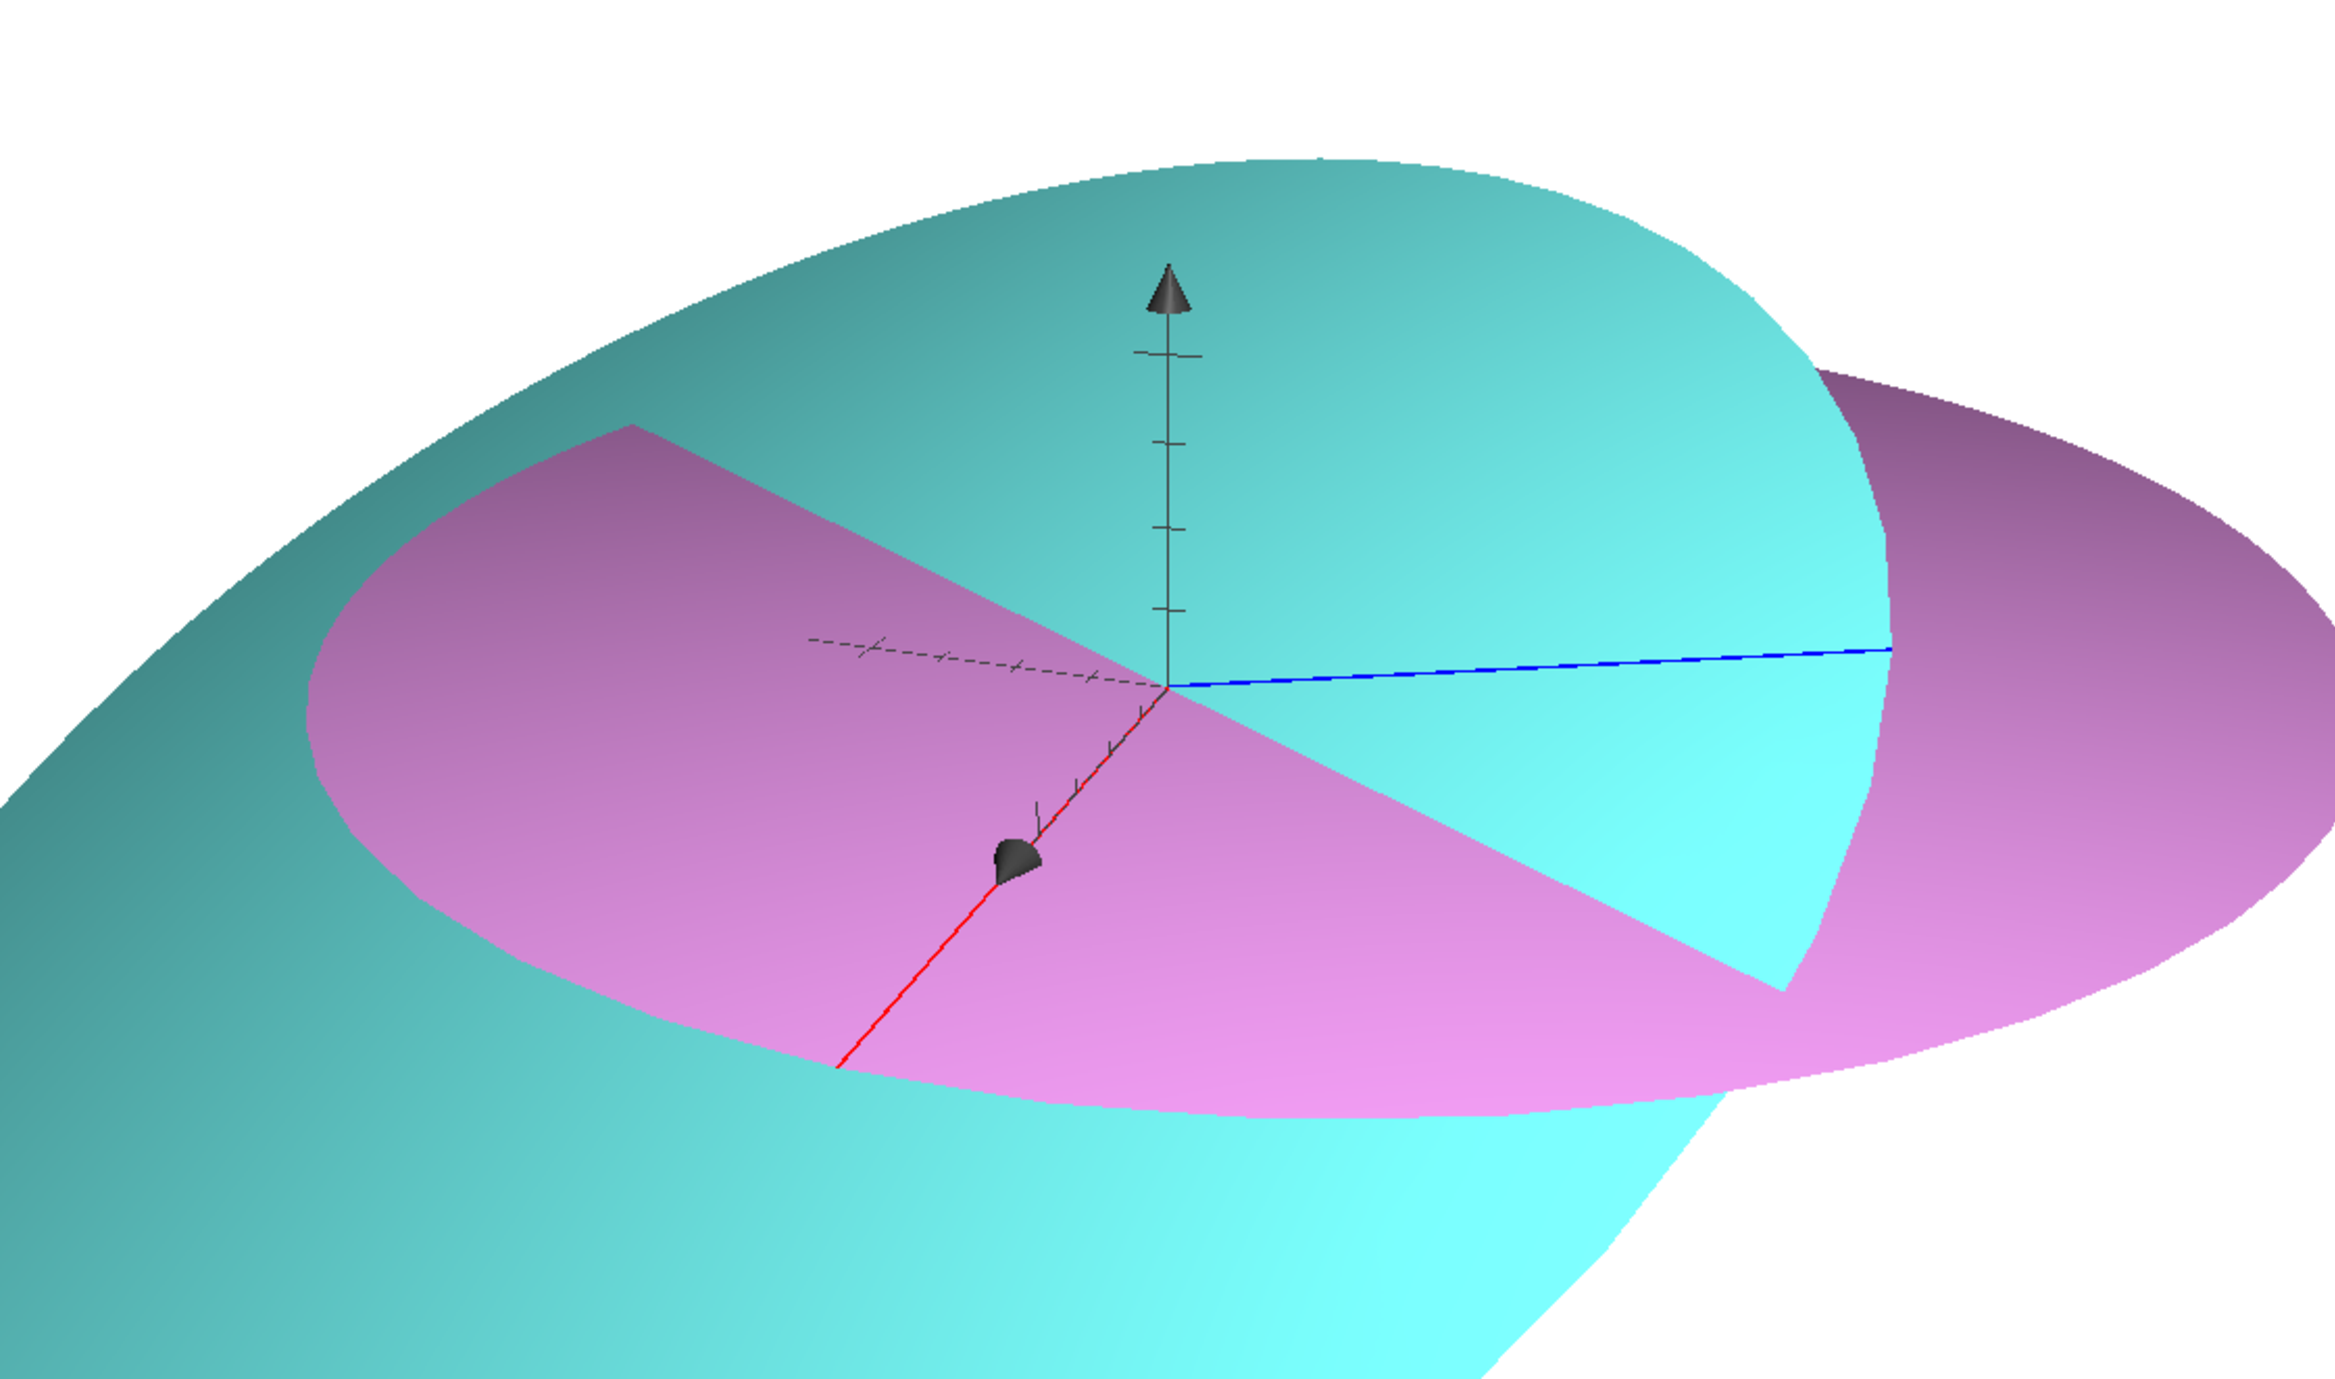
\includegraphics[width=7cm]{./image/ellipse4.pdf}
\end{minipage}
%
\end{tabular}
\caption{\label{fig:grapher}}
\end{figure}

これらのような3次元座標系の変換は,それぞれ ${\rm{\bm P}}_1,{\rm{\bm P}}_2,{\rm{\bm P}}_3$ のような3 $\times$ 3回転行列で表現できる.

\begin{equation}
{\rm{\bm P}}_1 =
\begin{pmatrix}
\cos \omega & - \sin \omega & 0\\
\sin \omega & \cos \omega & 0 \\
0 & 0 & 1\\
\end{pmatrix}
, \quad {\rm{\bm P}}_2 =
\begin{pmatrix}
1 & 0 & 0\\
0 & \cos I & - \sin I\\
0 & \sin I & \cos I\\
\end{pmatrix}
, \quad {\rm{\bm P}}_3 =
\begin{pmatrix}
\cos \Omega & - \sin \Omega & 0\\
\sin \Omega & \cos \Omega & 0 \\
0 & 0 & 1\\
\end{pmatrix}
\end{equation}

これらを使うと,
\begin{equation}
\begin{pmatrix}
X\\
Y\\
Z\\
\end{pmatrix}
= {\rm{\bm P}}_3 {\rm{\bm P}}_2 {\rm{\bm P}}_1
\begin{pmatrix}
x\\
y\\
z\\
\end{pmatrix}
\quad {\rm and} \quad
\begin{pmatrix}
x\\
y\\
z\\
\end{pmatrix}
= {\rm{\bm P}}_1^{-1} {\rm{\bm P}}_2^{-1} {\rm{\bm P}}_3^{-1}
\begin{pmatrix}
X\\
Y\\
Z\\
\end{pmatrix}
\end{equation}
ここで ${\rm{\bm P}}^{-1}$ は ${\rm{\bm P}}$ の逆行列である.すべての回転行列は直交行列であるため,逆行列は転置行列と等しい.

軌道面の座標系を基準面の座標系で表すと,
\begin{equation}
\begin{pmatrix}
X\\
Y\\
Z\\
\end{pmatrix}
= {\rm{\bm P}}_3 {\rm{\bm P}}_2 {\rm{\bm P}}_1
\begin{pmatrix}
r \cos f\\
r \sin f\\
0\\
\end{pmatrix}
= r 
\begin{pmatrix}
\cos \Omega \cos (\omega + f) - \sin \Omega \sin (\omega + f) \cos I\\
\sin \Omega \cos (\omega + f) + \cos \Omega \sin (\omega + f) \cos I\\
\sin (\omega + f) \sin I\\
\end{pmatrix}
\label{eq:xyzXYZ}
\end{equation}
回転変換では長さは保存されるため,$a, e$ の値は変化しない.

これで時間 $t$ での楕円運動をする天体の基準面の座標系における位置 ($X, Y, Z$) と速度 ($\dot{X}, \dot{Y}, \dot{Z}$) を,6つの軌道要素 $a, e, I, \Omega, \omega, f$ と近点通過時刻 $\tau$ に変換することができるようになった.中心星とそのまわりを回る天体の質量をそれぞれ $m_1, m_2$ とすると,
\begin{eqnarray}
R^2 & = & X^2 + Y^2 + Z^2, \label{eq:R}\\
V^2 & = & \dot{X}^2 + \dot{Y}^2 + \dot{Z}^2, \label{eq:Rdot}\\
{\bm R} \cdot \dot{{\bm R}} & = & X \dot{X} + Y \dot{Y} + Z \dot{Z}, \\
{\bm h} & = & (Y \dot{Z} - Z \dot{Y}, Z \dot{X} - X \dot{Z}, X \dot{Y} - Y \dot{X}), \\
\dot{R} & = & \pm \sqrt{V^2 - \frac{h^2}{R^2}}.
\end{eqnarray}
ここで $R = r$ は動径ベクトルの長さ,$\dot{R}$ はその変化率を示している.$R$ は常に正なので,$\dot{R}$ の符号は ${\bm R} \cdot \dot{{\bm R}}$ の符号と一致する.${\bm h} = (h_X, h_Y, h_Z)$ のそれぞれの成分は,
\begin{eqnarray}
h \cos I & = & h_Z, \label{eq:h_Z}\\
h \sin I \sin \Omega & = & \pm h_X, \label{eq:h_X}\\
h \sin I \cos \Omega & = & \mp h_Y. \label{eq:h_Y}
\end{eqnarray}
ここで,$h_Z$ の符号が正のとき (\ref{eq:h_X}),(\ref{eq:h_Y}) 式の上の符号,$h_Z$ の符号が負のとき下の符号をとる.

軌道要素を求める過程を以下に示す.

\begin{description}
\item[1)] (\ref{eq:v2new}),(\ref{eq:R}),(\ref{eq:Rdot}) 式から $a$ を求める.
\begin{equation}
a = \left( \frac{2}{R} -\frac{V^2}{G (m_1 + m_2)} \right)^{-1} \label{eq:axis}
\end{equation}
\item[2)] (\ref{eq:mu}),(\ref{eq:axis}) 式から $e$ を求める.
\begin{equation}
e = \sqrt{1- \frac{h^2}{G (m_1 + m_2) a}} \label{eq:ecc}
\end{equation}
\item[3)] (\ref{eq:h_Z}) 式から $I$ を求める.
\begin{equation}
I = \cos^{-1} \left( \frac{h_Z}{h} \right) \label{eq:inc}
\end{equation}
\item[4)] (\ref{eq:h_X}),(\ref{eq:h_Y}) 式から $\sin \Omega,\cos \Omega$ の形で $\Omega$ を求める.
\begin{equation}
\sin \Omega = \frac{\pm h_X}{h \sin I} \quad {\rm and} \quad \cos \Omega = \frac{\mp h_Y}{h \sin I}. \label{eq:OMEGA}
\end{equation}
符号は $h_Z$ の符号によって決まる.
\item[5)] (\ref{eq:xyzXYZ}) 式の $Z/R, X/R$ の表式から $\omega + f$ を求める.
\begin{equation}
\sin (\omega + f) = \frac{Z}{R \sin I} \quad {\rm and} \quad \cos (\omega + f) = \frac{1}{\cos \Omega} \left( \frac{X}{R} + \sin \Omega \sin (\omega + f) \cos I \right). \label{eq:omega+f}
\end{equation}
\item[6)] (\ref{eq:rf}),(\ref{eq:rdot}) 式から得られる $\sin f$ と $\cos f$ の表式から $f, \omega$ を求める.$\dot{r} = \dot{R}$ と置き換えると,
\begin{equation}
\sin f = \frac{a (1 - e^2)}{h e} \dot{R} \quad {\rm and} \quad \cos f = \frac{1}{e} \left( \frac{a (1 - e^2)}{R} - 1 \right). \label{eq:f}
\end{equation}
\item[7)] (\ref{eq:rE}) 式から $E$を計算し,(\ref{eq:mu}),(\ref{eq:tauE}) 式を用いて $\tau$ を求める.
\begin{equation}
\tau = t - \frac{E - e \sin E}{\sqrt{G (m_1 + m_2) a^{-3}}} \label{eq:tau}
\end{equation}
\end{description}

これらの式は軌道要素を求める正しい方法であるが,数値計算において,SI単位系や他の標準的な単位系よりも実用的な単位系を用いて,$G (m_1 + m_2) = 1$ とするように,すなわち時間 $t$ を $\sqrt{\mu} = \sqrt{G (m_1 + m_2)}$ でスケーリングし, 新たな時間 $\bar{t}$ を用いることがある.
\begin{equation}
\sqrt{\mu} dt = d \bar{t} \label{eq:tbar}
\end{equation}

(\ref{eq:raletive}) 式から,これは $\mu = 1$ としたときと同じである.加えて,単位長さを $a = 1$ と選ぶと,2体問題は単位平均運動 $n = 1$ と単位周期 $T = 2 \pi$ のケプラー運動として扱うことができる.これは円制限3体問題を扱う際にも同様の形で適用できる.


\section{制限3体問題 \label{sec:3body}}
この章では3体の物体が重力相互作用をした場合に拡張して考える.特に,3体目の質量が他の2つに比べ無視できるほど小さいときの3体目の物体の運動について考える.この問題は「制限3体問題」と呼ばれる.また,1,2体目の物体がそれらの共通重心を中心に円運動をし,3体目の物体がそれと同一な平面上を運動する場合,「円制限3体問題」と呼ばれる.一見すると,太陽系の天体運動に対して円制限3体問題はほとんど応用できないと思えるかもしれない.観測された太陽系の天体はやはり,同一平面上を運動せず円運動もしていない.しかし,太陽系の天体の軌道と質量の階層構造 (太陽,惑星,衛星,リングなど) は,制限3体問題がよい近似であり,比較的簡単な解析で定性的に天体の運動の振る舞いを理解できることを示している.

\subsection{運動方程式}
2つの質量 $m_1, m_2$ の物体の重力の影響下で,質量が無視できるほど小さい粒子の運動を考える.粒子は2つの物体に影響を与えないが,2つの物体は共通重心を中心に円運動をして粒子に力を及ぼすと仮定する.

$\xi, \eta, \zeta$ の軸を持ち,2つの物体の重心を原点にとる慣性座標系を考える (図 \ref{fig:xi_eta_zeta}).時刻 $t = 0$ で $m_1$ から $m_2$ に沿った方向に $\xi$ 軸,軌道平面上で $\xi$ 軸と垂直な方向に $\eta$ 軸,そして $\xi - \eta$ 平面に垂直な,角運動量ベクトルの方向に $\zeta$ 軸をとる.この慣性座標系での2つの物体の座標を ($\xi_1, \eta_1, \zeta_1$) ,($\xi_2, \eta_2, \zeta_2$) とし,距離は一定で,同じ角速度で共通重心のまわりを回っているとする.また単位質量を $\mu = G (m_1 + m_2) = 1$ となるように選ぶ.$m_1 > m_2$ と仮定し,
\begin{equation}
\bar{\mu} = \frac{m_2}{m_1 + m_2}
\end{equation}
と定義すると,この単位系での2つの物体の質量は,
\begin{equation}
\mu_1 = G m_1 = 1 - \bar{\mu} \quad {\rm and} \quad \mu_2 = G m_2 = \bar{\mu}, \label{eq:mu1mu2}
\end{equation}
となり,ここで仮定より $\bar{\mu} < 1/2$ である.単位長さは,2つの物体間の距離が1となるように選ぶ.そうすると,共通の平均運動 $n$ も1となる.

\begin{figure}[H]
\centering
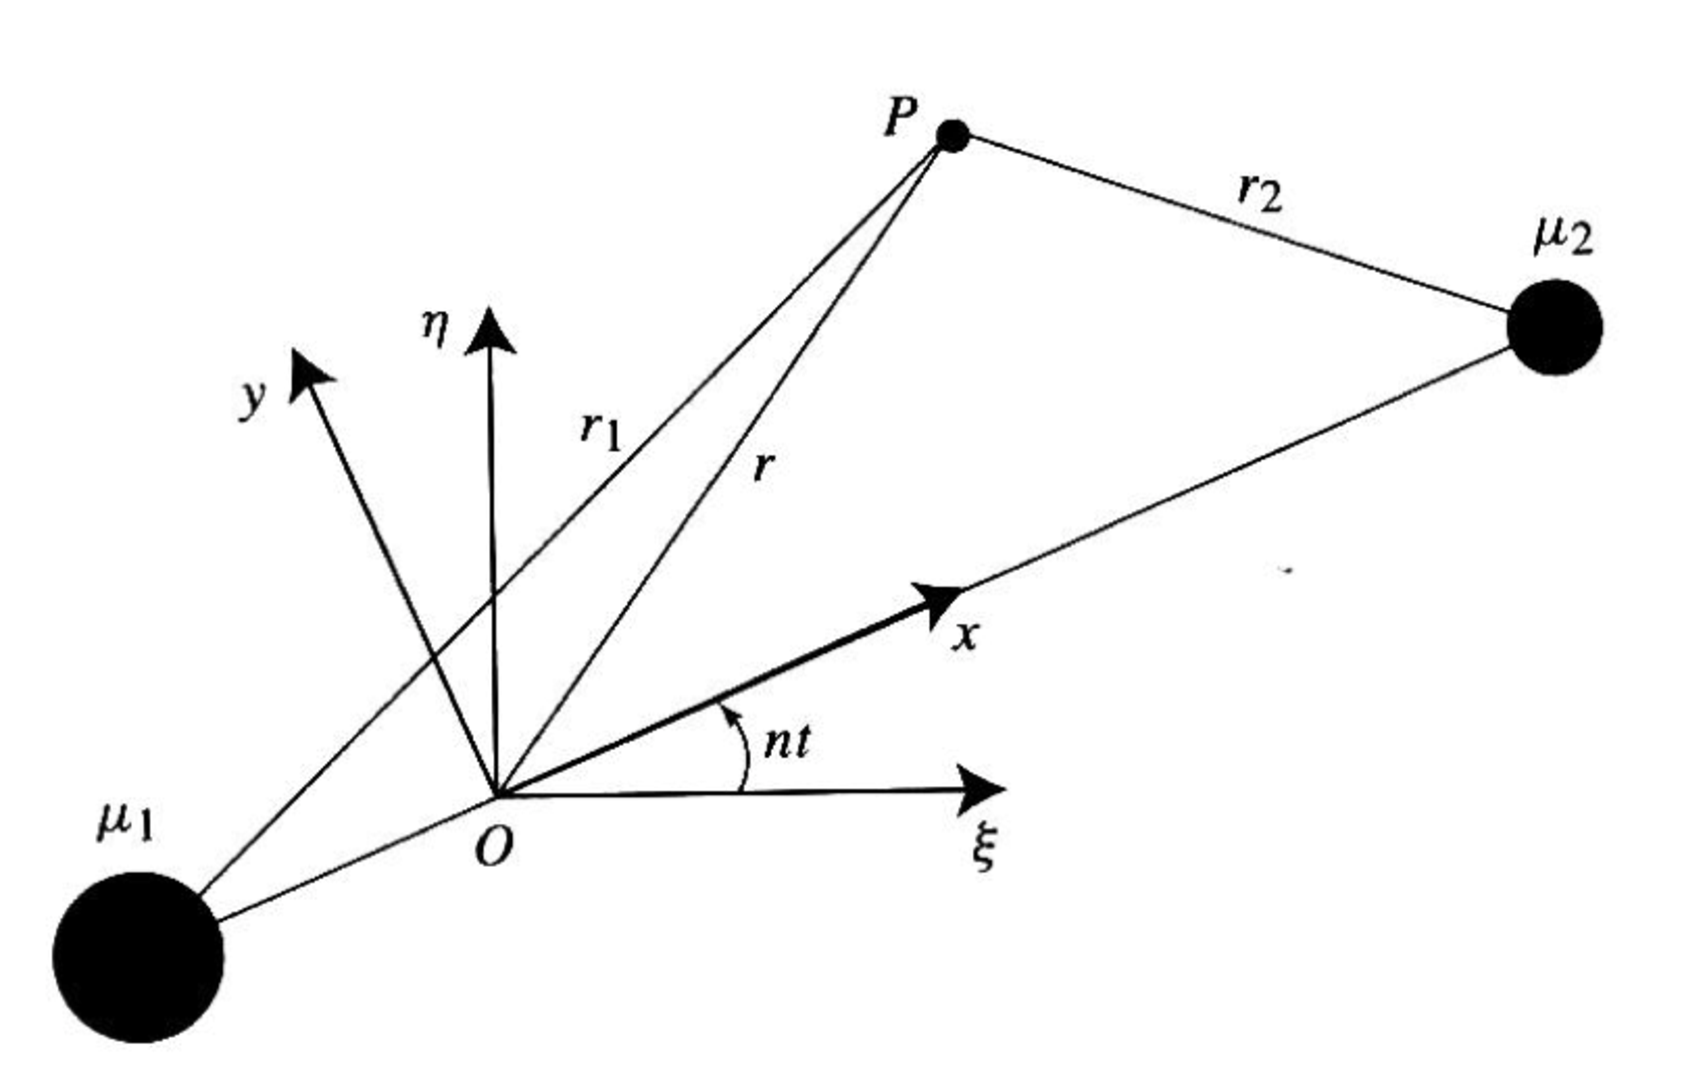
\includegraphics[width=10cm]{./image/sec3_1.pdf}
\caption{\label{fig:xi_eta_zeta}}
\end{figure}

慣性座標系,もしくは sidereal 座標系での粒子の座標を ($\xi, \eta, \zeta$) とする.逆2乗則のベクトル形式を用いると,
粒子の運動方程式は,
\begin{eqnarray}
\ddot{\xi} & = & \mu_1 \frac{\xi_1 - \xi}{r_1^3} + \mu_2 \frac{\xi_2 - \xi}{r_2^3}, \label{eq:xiddot}\\
\ddot{\eta} & = & \mu_1 \frac{\eta_1 - \eta}{r_1^3} + \mu_2 \frac{\eta_2 - \eta}{r_2^3}, \label{eq:etaddot}\\
\ddot{\zeta} & = & \mu_1 \frac{\zeta_1 - \zeta}{r_1^3} + \mu_2 \frac{\zeta_2 - \zeta}{r_2^3}, \label{eq:zetaddot}
\end{eqnarray}
となり,ここで図 \ref{fig:xi_eta_zeta} より,
\begin{eqnarray}
r_1^2 & = & (\xi_1 - \xi)^2 + (\eta_1 - \eta)^2 + (\zeta_1 - \zeta)^2,\\
r_2^2 & = & (\xi_2 - \xi)^2 + (\eta_2 - \eta)^2 + (\zeta_2 - \zeta)^2.
\end{eqnarray}
これらの方程式は,2つの物体の軌道の仮定が必要ないため,一般の3体問題にも有効である.

2つの物体が円運動をするとき,それらの距離と平均運動は一定である.このような場合,2つの物体の位置も固定されるような回転座標系での粒子の運動を考えたほうが自然である.ここで,$\xi, \eta$ 座標と原点は同じだが,正の方向に一定の回転速度 $n$ で回転する新たな座標系を考える (図 \ref{fig:xi_eta_zeta}).$x$ 軸を2つの物体に沿うようにとると,それぞれの座標は ($x_1, y_1,z_1$) = ($- \mu_2, 0, 0$),($x_2, y_2, z_2$) = ($\mu_1, 0, 0$) である.したがって,(\ref{eq:mu1mu2}) 式と図 \ref{fig:xi_eta_zeta} より,
\begin{eqnarray}
r_1^2 & = & (x + \mu_2)^2 + y^2 + z^2,\\
r_2^2 & = & (x - \mu_1)^2 + y^2 + z^2,
\end{eqnarray}
となり,ここで ($x, y, z$) は回転座標系,もしくは synodic 座標系での粒子の座標である.これらの座標系は次のような単純な回転で関連づけられる.
\begin{equation}
\begin{pmatrix}
\xi\\
\eta\\
\zeta\\
\end{pmatrix}
= 
\begin{pmatrix}
\cos nt & - \sin nt & 0\\
\sin nt & \cos nt & 0\\
0 & 0 & 1\\
\end{pmatrix}
\begin{pmatrix}
x\\
y\\
z\\
\end{pmatrix}. \label{eq:xi_eta_zeta_x_y_z}
\end{equation}
今用いている単位系では $n = 1$ であるが,方程式中に $n$ をあえて残しておく.

(\ref{eq:xi_eta_zeta_x_y_z}) 式を各成分ごとに2階微分すると,
\begin{equation}
\begin{pmatrix}
\dot{\xi}\\
\dot{\eta}\\
\dot{\zeta}\\
\end{pmatrix}
= 
\begin{pmatrix}
\cos nt & - \sin nt & 0\\
\sin nt & \cos nt & 0\\
0 & 0 & 1\\
\end{pmatrix}
\begin{pmatrix}
\dot{x} - ny\\
\dot{y} + nx\\
\dot{z}\\
\end{pmatrix} \label{eq:xidot_etadot_zetadot}
\end{equation}
and
\begin{equation}
\begin{pmatrix}
\ddot{\xi}\\
\ddot{\eta}\\
\ddot{\zeta}\\
\end{pmatrix}
= 
\begin{pmatrix}
\cos nt & - \sin nt & 0\\
\sin nt & \cos nt & 0\\
0 & 0 & 1\\
\end{pmatrix}
\begin{pmatrix}
\ddot{x} - 2 n \dot{y} - n^2 x\\
\ddot{y} + 2 n \dot{x} - n^2 y\\
\ddot{z}\\
\end{pmatrix}. \label{eq:xiddot_etaddot_zetaddot}
\end{equation}
回転座標系に切り替えることによって,$n \dot{x}, n \dot{y}$ の項 (コリオリ力) と $n^2 x, n^2 y$ の項 (遠心力) が運動方程式に生じる.これらの式を使って (\ref{eq:xiddot}),(\ref{eq:etaddot}),(\ref{eq:zetaddot}) 式を書き換えると,
\begin{equation}
\begin{split}
(\ddot{x} - 2 n \dot{y} & - n^2 x) \cos nt - (\ddot{y} + 2 n \dot{x} - n^2 y) \sin nt =\\
& \left[ \mu_1 \frac{x_1 - 1}{r_1^3} + \mu_2 \frac{x_2 - x}{r_2^3} \right] \cos nt + \left[ \frac{\mu_1}{r_1^3} + \frac{\mu_2}{r_2^3} \right] y \sin nt, \label{eq:cos_sin}
\end{split}
\end{equation}
\begin{equation}
\begin{split}
(\ddot{x} - 2 n \dot{y} & - n^2 x) \sin nt + (\ddot{y} + 2 n \dot{x} - n^2 y) \cos nt =\\
& \left[ \mu_1 \frac{x_1 - 1}{r_1^3} + \mu_2 \frac{x_2 - x}{r_2^3} \right] \sin nt - \left[ \frac{\mu_1}{r_1^3} + \frac{\mu_2}{r_2^3} \right] y \cos nt, \label{eq:sin_cos}
\end{split}
\end{equation}
\begin{equation}
\ddot{z} = - \left[ \frac{\mu_1}{r_1^3} + \frac{\mu_2}{r_2^3} \right] z.
\end{equation}
(\ref{eq:cos_sin}) 式と $\cos nt$ の積,(\ref{eq:sin_cos}) 式と $\sin nt$ の積の和をとり,また (\ref{eq:cos_sin}) 式と $- \sin nt$ の積,(\ref{eq:sin_cos}) 式と $\cos nt$ の積の和をとると,synodic 座標系での運動方程式は,
\begin{eqnarray}
\ddot{x} - 2 n \dot{y} - n^2 x & = & - \left[ \mu_1 \frac{x + \mu_2}{r_1^3} + \mu_2 \frac{x - \mu_1}{r_2^3} \right],\\
\ddot{y} + 2 n \dot{x} - n^2 y & = & - \left[ \frac{\mu_1}{r_1^3} + \frac{\mu_2}{r_2^3} \right] y,\\
\ddot{z} & = & - \left[ \frac{\mu_1}{r_1^3} + \frac{\mu_2}{r_2^3} \right] z.
\end{eqnarray}
これらの運動方程式はスカラー関数 $U$ の勾配として書くこともできる.
\begin{eqnarray}
\ddot{x} - 2 n \dot{y} & = & \frac{\partial U}{\partial x}, \label{eq:xU}\\
\ddot{y} + 2 n \dot{x} & = & \frac{\partial U}{\partial y}, \label{eq:yU}\\
\ddot{z} & = & \frac{\partial U}{\partial z}. \label{eq:zU}
\end{eqnarray}
ここで $U = U (x, y, z)$ は次のように与えられる.
\begin{equation}
U = \frac{n^2}{2} (x^2 + y^2) + \frac{\mu_1}{r_1} + \frac{\mu_2}{r_2}. \label{eq:U}
\end{equation}
$x^2 + y^2$ の項は遠心力によるポテンシャル,$1/r_1, 1/r_2$ の項は重力によるポテンシャルであり,それぞれの偏微分をとると運動方程式に遠心力,重力の項が現れる.

(\ref{eq:xU}),(\ref{eq:yU}) 式の $- 2n \dot{y}$ と $+ 2n \dot{x}$ の項はコリオリ項であり,回転座標系での粒子の速度に依存する.コリオリ力は速度方向に対して右側にずれる力であり,ゆえに効かない.

$U$ の定義より符号は正であるが,単に天文学の伝統であり,物理では慣習として符号を負にする.$U^{\ast} = - U$ のように置き換えると運動方程式は,
\begin{eqnarray}
\ddot{x} - 2 n \dot{y} & = & - \frac{\partial U^{\ast}}{\partial x}, \label{eq:xUast}\\
\ddot{y} + 2 n \dot{x} & = & - \frac{\partial U^{\ast}}{\partial y}, \label{eq:yUast}\\
\ddot{z} & = & - \frac{\partial U^{\ast}}{\partial z}. \label{eq:zUast}
\end{eqnarray}
また,$U$ は真のポテンシャルではなく,回転座標系での粒子にかかる力のいくつか (全てではない) を得ることができるスカラー関数である.$U$ は偽ポテンシャルと呼ぶ.

\subsection{Jacobi積分}
(\ref{eq:xU}) 式と $\dot{x}$ の積,(\ref{eq:yU}) 式と $\dot{y}$ の積,(\ref{eq:zU}) 式と $\dot{z}$ の積の和をとると,
\begin{equation}
\dot{x} \ddot{x} + \dot{y} \ddot{y} + \dot{z} \ddot{z} = \frac{\partial U}{\partial x} \dot{x} + \frac{\partial U}{\partial y} \dot{y} + \frac{\partial U}{\partial z} \dot{z} = \frac{dU}{dt}.
\end{equation}
これは積分できて,
\begin{equation}
\dot{x}^2 + \dot{y}^2 + \dot{z}^2 = 2 U - C_J, \label{eq:2U-C_J}
\end{equation}
ここで $C_J$ は積分定数である.$\dot{x}^2 + \dot{y}^2 + \dot{z}^2 = v^2$ は回転座標系での速度の2乗なので,
\begin{equation}
v^2 = 2 U - C_J
\end{equation}
または,(\ref{eq:U}) 式を用いて,
\begin{equation}
C_J = n^2 (x^2 + y^2) + 2 \left( \frac{\mu_1}{r_1} + \frac{\mu_2}{r_2} \right) - \dot{x}^2 - \dot{y}^2 - \dot{z}^2.
\end{equation}
これらのことから,$2 U - C_J$ はこの運動における定数であることがわかる.これはJacobi積分,またはJacobi定数であり,時には相対エネルギー積分とも呼ばれる.ただし,制限3体問題ではエネルギーも角運動量も保存しないので,エネルギー積分ではないことに注意する.Jacobi積分は単に円制限3体問題における積分定数であり,これは一般の場合には3体問題は閉じた式で解くことはできないことを意味する.

$C_J$ の表式は,回転していない,sidereal 座標系での粒子の位置と速度を使って書くこともできる.位置ベクトルは, (\ref{eq:xi_eta_zeta_x_y_z}) 式を用いると,
\begin{equation}
\begin{pmatrix}
x\\
y\\
z\\
\end{pmatrix}
= 
\begin{pmatrix}
\cos nt & \sin nt & 0\\
- \sin nt & \cos nt & 0\\
0 & 0 & 1\\
\end{pmatrix}
\begin{pmatrix}
\xi\\
\eta\\
\zeta\\
\end{pmatrix}. \label{eq:x_y_z_xi_eta_zeta}
\end{equation}
速度ベクトルは,(\ref{eq:xidot_etadot_zetadot}) 式を用いると,
\begin{equation}
\begin{pmatrix}
\dot{x} - ny\\
\dot{y} + nx\\
\dot{z}\\
\end{pmatrix}
= 
\begin{pmatrix}
\cos nt & \sin nt & 0\\
- \sin nt & \cos nt & 0\\
0 & 0 & 1\\
\end{pmatrix}
\begin{pmatrix}
\dot{\xi}\\
\dot{\eta}\\
\dot{\zeta}\\
\end{pmatrix} \label{eq:xdot_ydot_zdot_1}
\end{equation}
しかし,
\begin{equation}
\begin{pmatrix}
\dot{x} - ny\\
\dot{y} + nx\\
\dot{z}\\
\end{pmatrix}
= 
\begin{pmatrix}
\dot{x}\\
\dot{y}\\
\dot{z}\\
\end{pmatrix}
+ n
\begin{pmatrix}
\sin nt & - \cos nt & 0\\
\cos nt & \sin nt & 0\\
0 & 0 & 0\\
\end{pmatrix}
\begin{pmatrix}
\xi\\
\eta\\
\zeta\\
\end{pmatrix} \label{eq:xdot_ydot_zdot_2}
\end{equation}
とも書けるから,したがって,
\begin{equation}
\begin{pmatrix}
\dot{x}\\
\dot{y}\\
\dot{z}\\
\end{pmatrix}
= 
\begin{pmatrix}
\cos nt & \sin nt & 0\\
- \sin nt & \cos nt & 0\\
0 & 0 & 1\\
\end{pmatrix}
\begin{pmatrix}
\dot{\xi}\\
\dot{\eta}\\
\dot{\zeta}\\
\end{pmatrix}
- n
\begin{pmatrix}
\sin nt & - \cos nt & 0\\
\cos nt & \sin nt & 0\\
0 & 0 & 0\\
\end{pmatrix}
\begin{pmatrix}
\xi\\
\eta\\
\zeta\\
\end{pmatrix} \label{eq:xdot_ydot_zdot_3}
\end{equation}
ここで,
\begin{equation}
{\rm A} = 
\begin{pmatrix}
\cos nt & \sin nt & 0\\
- \sin nt & \cos nt & 0\\
0 & 0 & 1\\
\end{pmatrix}
 \quad {\rm and} \quad 
 {\rm B} = 
\begin{pmatrix}
\sin nt & - \cos nt & 0\\
\cos nt & \sin nt & 0\\
0 & 0 & 0\\
\end{pmatrix}
\end{equation}
とおくと,(\ref{eq:xdot_ydot_zdot_3}) 式から,
\begin{equation}
\begin{split}
\dot{x}^2 + \dot{y}^2 + \dot{z}^2 & = 
\begin{pmatrix}
\dot{x} & \dot{y} & \dot{z}\\
\end{pmatrix}
\begin{pmatrix}
\dot{x}\\
\dot{y}\\
\dot{z}\\
\end{pmatrix}\\
& = 
\begin{pmatrix}
\dot{\xi} & \dot{\eta} & \dot{\zeta}\\
\end{pmatrix}
{\rm A}^{\rm T} {\rm A} 
\begin{pmatrix}
\dot{\xi}\\
\dot{\eta}\\
\dot{\zeta}\\
\end{pmatrix}
- n
\begin{pmatrix}
\dot{\xi} & \dot{\eta} & \dot{\zeta}\\
\end{pmatrix}
{\rm A}^{\rm T} {\rm B} 
\begin{pmatrix}
\xi\\
\eta\\
\zeta\\
\end{pmatrix}\\
& \quad - n
\begin{pmatrix}
\xi & \eta & \zeta\\
\end{pmatrix}
{\rm B}^{\rm T} {\rm A}
 \begin{pmatrix}
\dot{\xi}\\
\dot{\eta}\\
\dot{\zeta}\\
\end{pmatrix}
+ n^2 
\begin{pmatrix}
\xi & \eta & \zeta\\
\end{pmatrix}
{\rm B}^{\rm T} {\rm B}
\begin{pmatrix}
\xi\\
\eta\\
\zeta\\
\end{pmatrix}\\
& =  \dot{\xi}^2 + \dot{\eta}^2 + \dot{\zeta}^2 + n^2 (\xi^2 + \eta^2) + 2 n (\dot{\xi} \eta - \dot{\eta} \xi)
\end{split}
\end{equation}
ここで,${\rm A}^{\rm T}, {\rm B}^{\rm T}$ は ${\rm A}, {\rm B}$ の転置行列を表す.${\rm A}, {\rm B}$ はどちらも直交行列なので,逆行列は単純に自身の転置行列である.回転行列を作用させても距離は常に変わらないので (言い換えると,直交行列の行列式は$\pm 1$なので),$x^2 + y^2 + z^2 = \xi^2 + \eta^2 + \zeta^2$ である.このことは,(\ref{eq:xi_eta_zeta_x_y_z}) 式からも得られる.したがって,sidereal 座標系でのJacobi積分の表式は,
\begin{equation}
C_J = 2 \left( \frac{\mu_1}{r_1} + \frac{\mu_2}{r_2} \right) + 2 n (\dot{\xi} \eta - \dot{\eta} \xi) - \dot{\xi}^2 - \dot{\eta}^2 - \dot{\zeta}^2 \label{eq:C_J}
\end{equation}
となる.これは以下のように書き直せる.
\begin{equation}
 \frac{1}{2} (\dot{\xi}^2 + \dot{\eta}^2 + \dot{\zeta}^2) - \left( \frac{\mu_1}{r_1} + \frac{\mu_2}{r_2} \right) = {\bm h} \cdot {\bm n} - \frac{1}{2} C_J
\end{equation}
ここで ${\bm n} = (0, 0, n)$ であり,左辺は粒子の単位質量あたりの全エネルギーである.${\bm h} \cdot {\bm n}$ は一定ではないため,制限3体問題ではエネルギーが保存しない理由はこの式で説明できる.

各座標系での粒子の位置と速度を測定することで,粒子の運動と関連したJacobi積分の値を決定することができる.2体問題では,角運動量とエネルギー積分を使って相対運動を解くことができた.Jacobi積分は制限3体問題の単なる積分定数である.Jacobi積分を使って運動を厳密に解くことはできないが,粒子が存在できない領域を決定することができる.

\begin{figure}[H]
\centering
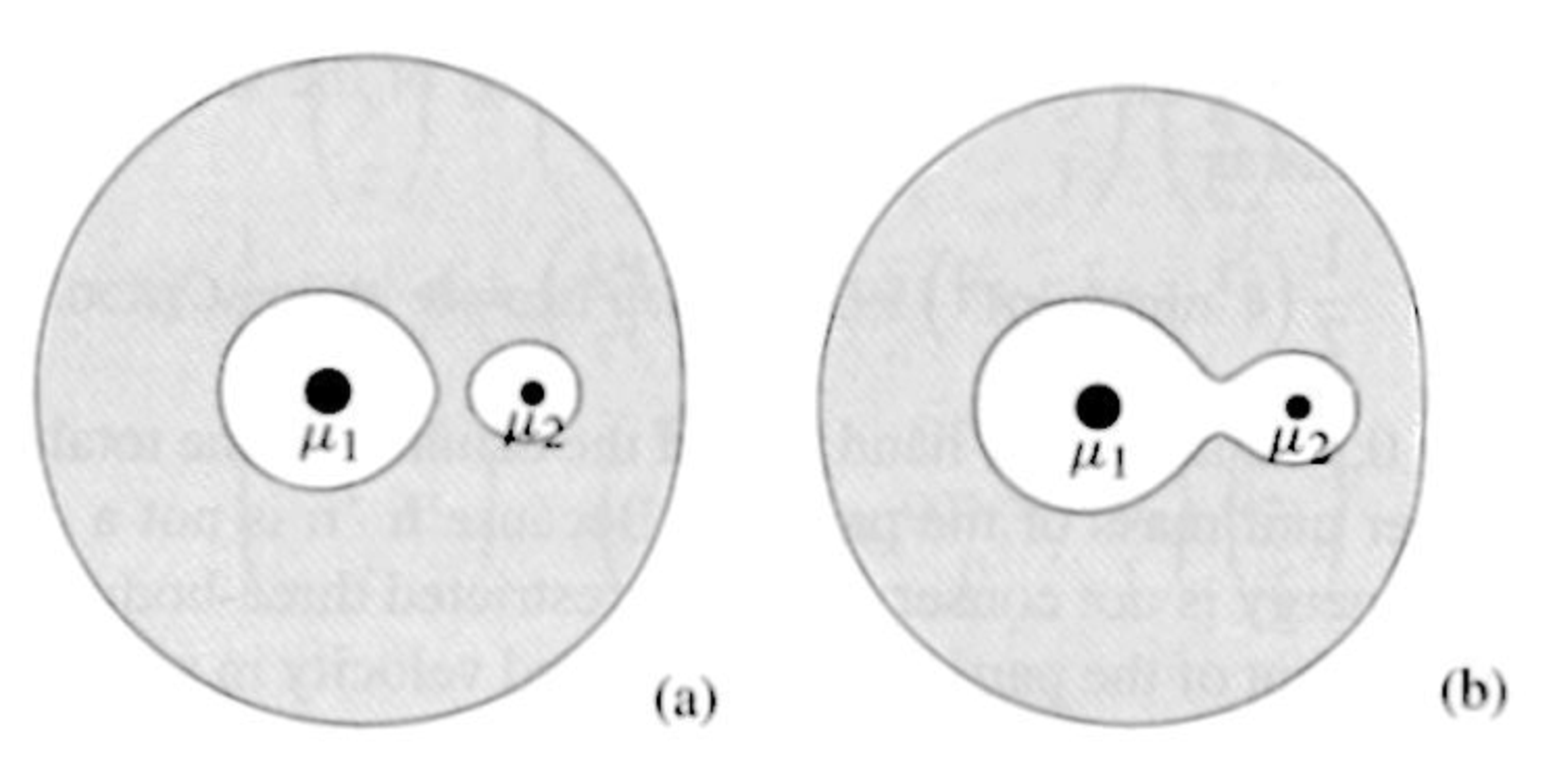
\includegraphics[width=10cm]{./image/sec3_2.pdf}
\caption{\label{fig:zerovelo}}
\end{figure}

粒子の速度が0である場所を考えることで,Jacobi積分の有用さがわかる.この場合,
\begin{equation}
2 U = C_J
\end{equation}
または,
\begin{equation}
n^2 (x^2 + y^2) + 2 \left( \frac{\mu_1}{r_1} + \frac{\mu_2}{r_2} \right) = C_J \label{eq:zerovelo}
\end{equation}
(\ref{eq:zerovelo}) 式はある $C_J$ の値の曲面を定義している.この曲面はゼロ速度曲面として知られているもので,粒子の運動に制約を与える上で重要な役割を果たす.簡単のため $x-y$ 平面を考えると,ゼロ速度曲面と $x-y$ 平面が交わるところでは,ゼロ速度曲線を形成する.図 \ref{fig:zerovelo} は $\mu_2 = 0.2, n = 1$ の場合のゼロ速度曲線を示している.(\ref{eq:2U-C_J}) 式から,常に $2 U \hspace{0.3em}\raisebox{0.4ex}{$>$}\hspace{-0.75em}\raisebox{-.7ex}{=}\hspace{0.3em} C_J$ であることは明らかである.ゆえに(\ref{eq:zerovelo}) 式は,粒子が運動が不可能な領域の境界線を決定する.したがって,制限3体問題は積分不可能である (任意の初期状態から粒子の運動を解くことができない) が,Jacobi積分が存在することによって,粒子が存在できない $x-y$ 平面の領域を見つけることができる.この結果は簡単に3次元に拡張できる.

\subsection{Tissrand Relation}
軌道長半径 $a$,離心率 $e$,軌道傾斜角 $I$ をもつ彗星を考える.また,この彗星が木星に接近した後の軌道要素を $a', e', I'$ とする.これらの2組の軌道要素は,Jacobi積分やいくつかの近似を用いることで簡単に関連づけることができる.Jacobi積分の値 $C_J = 2 U - v^2$ は接近の間定数である.3次元慣性座標系では,彗星は位置ベクトル ${\bm r} = (\xi, \eta, \zeta)$,速度ベクトル $\dot{{\bm r}} = (\dot{\xi}, \dot{\eta}, \dot{\zeta})$ を持つ.この座標系では,(\ref{eq:C_J}) 式よりJacobi積分を以下のように書くことができる.
\begin{equation}
C_J = 2 \left( \frac{\mu_1}{r_1} + \frac{\mu_2}{r_2} \right) + 2 n (\dot{\xi} \eta - \dot{\eta} \xi) - \dot{\xi}^2 - \dot{\eta}^2 - \dot{\zeta}^2 \label{eq:C_Jcomet}
\end{equation}
ここで $r_1, r_2$ はそれぞれ彗星の太陽からと木星からの距離である.木星の軌道長半径を単位長さ,木星の平均運動を単位角速度として選ぶ.また木星と彗星の質量は太陽に比べ十分に小さいため,
\begin{equation}
G (m_{\rm sun} + m_{\rm comet}) \approx G (m_{\rm sun} + m_{\rm Jupiter}) = 1
\end{equation}
ここで $m_{\rm sun}, m_{\rm comet}, m_{\rm Jupiter}$ はそれぞれ太陽,彗星,木星の質量である.太陽-彗星の2体問題のエネルギー積分は (\ref{eq:v2new}) 式より,
\begin{equation}
\dot{\xi}^2 + \dot{\eta}^2 + \dot{\zeta}^2 = \frac{2}{r} - \frac{1}{a}
\end{equation}
ここで選んだ単位系では $\mu = 1$ であり,また木星と彗星の質量は太陽に比べ無視できるため,$r_1 \approx r$ と仮定した.彗星の単位質量あたりの角運動量は,
\begin{equation}
{\bm h} = {\bm r} \times \dot{{\bm r}}
\end{equation}
木星の軌道面に対する彗星の軌道傾斜角を $I$ とすると,角運動量の $\zeta$ 成分は,
\begin{equation}
\xi \dot{\eta} - \eta \dot{\xi} = h \cos I
\end{equation}
ここで選んだ単位系では $h^2 = a (1 - e^2)$ である.したがって,(\ref{eq:C_Jcomet}) 式のJacobi積分の表式から,
\begin{equation}
\frac{2}{r} - \frac{1}{a} - 2 \sqrt{a (1 - e^2)} \cos I = \frac{2}{r} - 2 \mu_2 \left( \frac{1}{r} - \frac{1}{r_2} \right) - C_J
\end{equation}
彗星が木星から遠く $1/r_2$ が常に微少量だとし,$\mu_2$ の項を無視すると,
\begin{equation}
\frac{1}{2a} + \sqrt{a (1 - e^2)} \cos I \approx {\rm const.}
\end{equation}
したがって,彗星の木星接近前後の軌道要素の関係は,近似的に以下のように書くことができる.
\begin{equation}
\frac{1}{2a} + \sqrt{a (1 - e^2)} \cos I = \frac{1}{2a'} + \sqrt{a' (1 - e'^2)} \cos I'
\end{equation}
これはTisserand relation (Tisserand 1896) として知られ,新しく発見された彗星が,惑星に接近して軌道要素を変えられたすでに発見されていた彗星かどうかを判定するのに使うことができる.

\section{摂動関数}
\ref{sec:3body} 章では,制限問題における惑星の位置から3体問題を扱った.しかし,任意の初期条件で2つの物体から重力の影響を受ける,3体目の物体の運動のより一般的な問題に取り組もうとはしなかった.この問題は積分不可能であるが,3体目の物体が受ける加速度を解析することで議論を進めることができる.運動が中心星または主星に支配されているなら,伴星らの軌道は,相互重力摂動によって円錐曲線から少しずれたものとなる.この章では,摂動関数 (disturbing function) の定義と解析によって,このずれがどのように計算できるのかを示す.

質量 $m_c$ の主星のまわりを質量 $m_i$ の天体が楕円軌道で回っている場合を考える.\ref{sec:2body} 章でみてきたように,この2体問題は積分可能であり,主星の重力効果が質点によるものみなすと,$m_i$ の天体の軌道要素 $a_i, e_i, I_i, \varpi_i, \Omega_i$ は定数である.ここで3体目の天体 $m_j$ を導入すると,$m_c$ との2体問題での加速度に加えて,$m_i$ と $m_j$ 間の相互重力が加速度に足される (図 \ref{fig:disturbingfunc}).主星に対する伴星らの相対的な追加の加速度は,摂動関数と呼ばれる摂動のポテンシャルの勾配から得られる.

この章は,摂動関数のフーリエ級数展開の性質の数学的な解析と関係している.摂動関数の展開式から適切な項を取り出し,その他の項の運動方程式への時間平均された寄与が無視できると仮定し,太陽系力学における特定の問題に取り組む方法を示す.摂動関数の性質を理解することは,太陽系における共鳴の力学やその他の長周期運動を理解する鍵となる.

\begin{figure}[H]
\centering
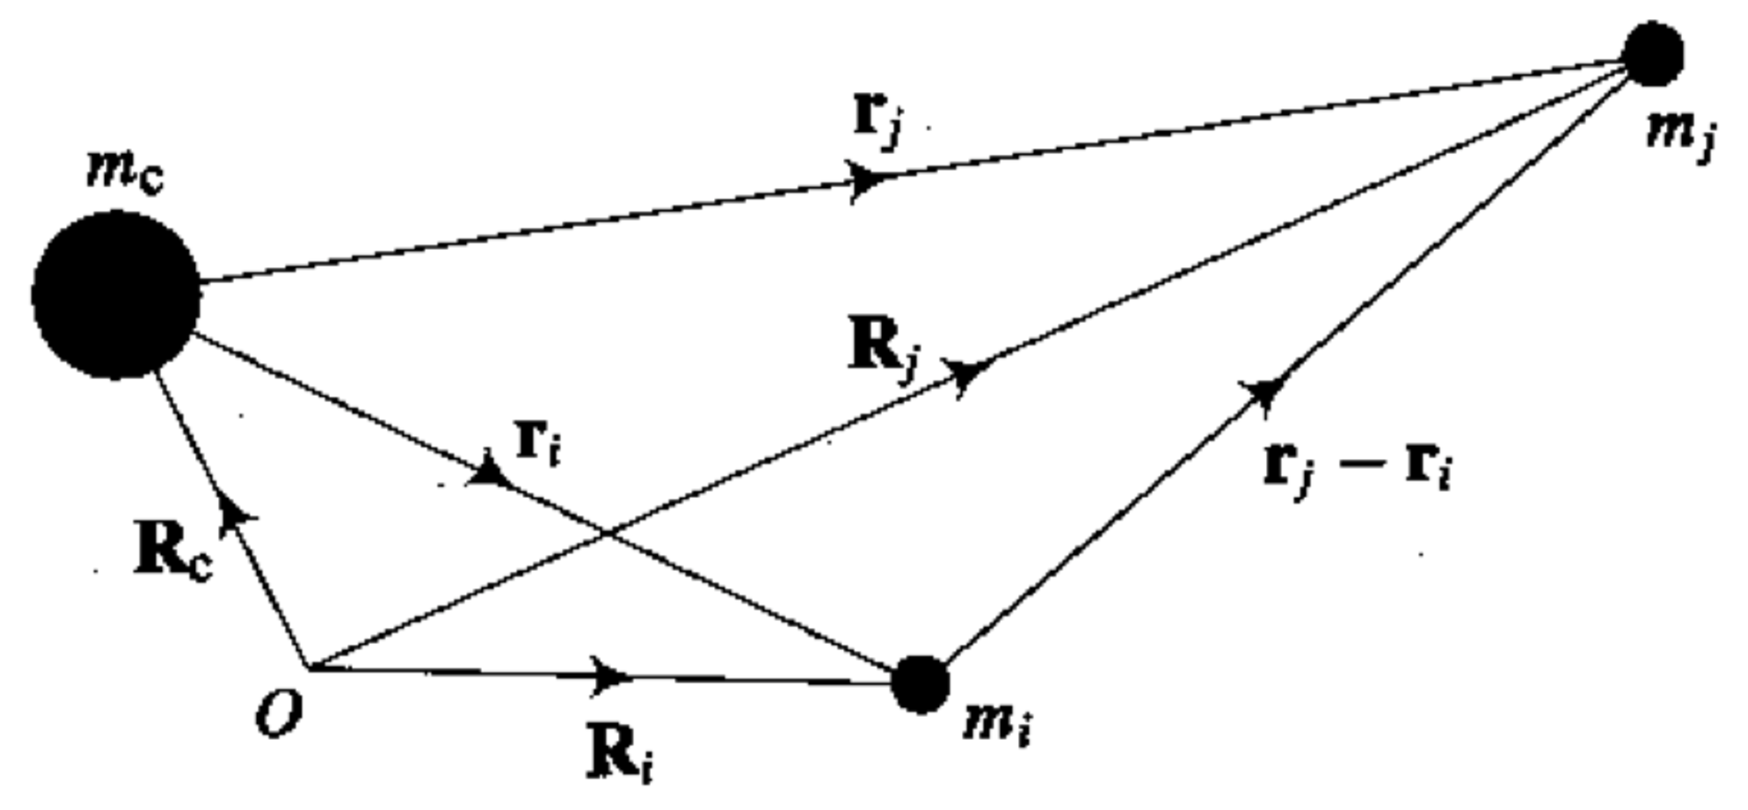
\includegraphics[width=10cm]{./image/sec6_1.pdf}
\caption{\label{fig:disturbingfunc}}
\end{figure}

\subsection{摂動関数}
質量 $m_c, m_i, m_j$ の3つの天体の,固定された原点 $O$ に対する位置ベクトルをそれぞれ ${\bm R}_c, {\bm R}_i, {\bm R}_j$ とする.主星 $m_c$ に対する伴星 $m_i, m_j$ の位置ベクトルをそれぞれ ${\bm r}_i, {\bm r}_j$ とすると,
\begin{equation}
|{\bm r}_i| = r_i = (x_i^2 + y_i^2 + z_i^2)^{1/2}, \quad |{\bm r}_j| = r_j = (x_j^2 + y_j^2 + z_j^2)^{1/2},
\end{equation}
そして
\begin{equation}
|{\bm r}_j- {\bm r}_i| = \left[ (x_j - x_i)^2 + (y_j - y_i)^2 + (z_j - z_i)^2 \right]^{1/2}.
\end{equation}
この座標系の原点は主星である (図 \ref{fig:disturbingfunc}).

ニュートンの運動の法則と重力の法則より,慣性系における3つの天体の運動方程式が得られる.
\begin{eqnarray}
m_c \ddot{\bm R}_c & = & G m_c m_i \frac{{\bm r}_i}{r_i^3} + G m_c m_j \frac{{\bm r}_j}{r_j^3}, \label{eq:R_c}\\
m_i \ddot{\bm R}_i & = & G m_i m_j \frac{({\bm r}_j - {\bm r}_i)}{|{\bm r}_j - {\bm r}_i|^3} - G m_i m_c \frac{{\bm r}_i}{r_i^3}, \label{eq:R_i}\\
m_j \ddot{\bm R}_j & = & G m_j m_i \frac{({\bm r}_i - {\bm r}_j)}{|{\bm r}_i - {\bm r}_j|^3} - G m_j m_c \frac{{\bm r}_j}{r_j^3}. \label{eq:R_j}
\end{eqnarray}
主星に対する伴星の加速度は以下のように与えられる.
\begin{eqnarray}
\ddot{\bm r}_i & = & \ddot{\bm R}_i - \ddot{\bm R}_c, \\
\ddot{\bm r}_j & = & \ddot{\bm R}_j - \ddot{\bm R}_c.
\end{eqnarray}
(\ref{eq:R_c}),(\ref{eq:R_i}),(\ref{eq:R_j}) 式から $\ddot{\bm R}_c, \ddot{\bm R}_i, \ddot{\bm R}_j$ の表式を代入すると,
\begin{eqnarray}
\ddot{\bm r}_i + G (m_c + m_i) \frac{{\bm r}_i}{r_i^3} & = & G m_j \left( \frac{{\bm r}_j - {\bm r}_i}{| {\bm r}_j - {\bm r}_i |^3} - \frac{{\bm r}_j}{r_j^3} \right), \label{eq:r_i} \\ 
\ddot{\bm r}_j + G (m_c + m_j) \frac{{\bm r}_j}{r_j^3} & = & G m_i \left( \frac{{\bm r}_i - {\bm r}_j}{| {\bm r}_i - {\bm r}_j |^3} - \frac{{\bm r}_i}{r_i^3} \right). \label{eq:r_j}
\end{eqnarray}
これらの相対加速度は,スカラー関数の勾配として以下のように書ける.
\begin{eqnarray}
\ddot{\bm r}_i & = & \nabla_i (U_i + {\cal R}_i) = \left( \hat{\bf i} \frac{\partial}{\partial x_i} + \hat{{\bf j}} \frac{\partial}{\partial y_i} + \hat{\bf k} \frac{\partial}{\partial z_i} \right) (U_i + {\cal R}_i), \label{eq:r_i_nabla} \\ 
\ddot{\bm r}_j & = & \nabla_j (U_j + {\cal R}_j) = \left( \hat{\bf i} \frac{\partial}{\partial x_j} + \hat{{\bf j}} \frac{\partial}{\partial y_j} + \hat{\bf k} \frac{\partial}{\partial z_j} \right) (U_j + {\cal R}_j), \label{eq:r_j_nabla}
\end{eqnarray}
ここで,
\begin{equation}
U_i = G \frac{m_c + m_i}{r_i} \quad {\rm and} \quad U_j = G \frac{m_c + m_j}{r_j}
\end{equation}
は全体のポテンシャルのうちの2体問題の部分である.$\nabla$ 演算子の添字 $i, j$ は,勾配を $m_i, m_j$ それぞれの座標についてとることを強調している.ポテンシャル中の${\cal R}$ の項は摂動関数であり,他の伴星によって生じるポテンシャルを表している.${\bm r}_i$ は $x_j, y_j, z_j$ によらず,${\bm r}_j$ は $x_i, y_i, z_i$ によらないので,以下のように書ける.
\begin{eqnarray}
{\cal R}_i & = & \frac{G m_j}{ |{\bm r}_j - {\bm r}_i| } - G m_j \frac{ {\bm r}_i \cdot {\bm r}_j }{r_j^3}, \\
{\cal R}_j & = & \frac{G m_i}{ |{\bm r}_i - {\bm r}_j| } - G m_i \frac{ {\bm r}_i \cdot {\bm r}_j }{r_i^3}.
\end{eqnarray}
第一項は直接項 (direct terms) と呼ばれ,座標系の原点のとり方によって生じる第二項は間接項 (indirect terms) と呼ばれる.座標系の原点が重心にある場合,この間接項は現れない.

上記の解析は天体の数を増やしても拡張できる.さらに,摂動関数に関係した加速度は,質点の重力に限らずどのような原因からでも生じうる.例えば,主星の扁平性によるポテンシャルから生じる.ここから先,この章では,質量がそれぞれ $m, m'$ で主星に対する位置ベクトルがそれぞれ ${\bm r}, {\bm r'}$ である2つの伴星を質点とみなす特別な場合を主に考える.ここで常に $r < r'$ とする.このとき,内側の伴星の運動方程式は,
\begin{equation}
\ddot{\bm r} + G (m_c + m) \frac{{\bm r}}{r^3} = G m' \left( \frac{{\bm r'} - {\bm r}}{| {\bm r'} - {\bm r} |^3} - \frac{{\bm r'}}{r'^3} \right)
\end{equation}
そして内側の伴星の摂動関数は,
\begin{equation}
{\cal R} = \frac{\mu'}{ |{\bm r'} - {\bm r}| } - \mu' \frac{ {\bm r} \cdot {\bm r'} }{r'^3}
\end{equation}
ここで $\mu' = G m'$ であり,内側の伴星の基準軌道は接触軌道要素 $n^2 a^3 = G (m_c + m)$ を持つ.同様に外側の伴星に関する運動方程式は,
\begin{equation}
\ddot{\bm r'} + G (m_c + m') \frac{{\bm r'}}{r'^3} = G m \left( \frac{{\bm r} - {\bm r'}}{| {\bm r} - {\bm r'} |^3} - \frac{{\bm r}}{r^3} \right)
\end{equation}
そして外側の伴星の摂動関数は,
\begin{equation}
{\cal R'} = \frac{\mu}{ |{\bm r} - {\bm r'}| } - \mu \frac{ {\bm r} \cdot {\bm r'} }{r^3}
\end{equation}
ここで $\mu = G m$ であり,外側の伴星の基準軌道は接触軌道要素 $n'^2 a'^3 = G (m_c + m')$ を持つ.












\begin{figure}[H]
\centering
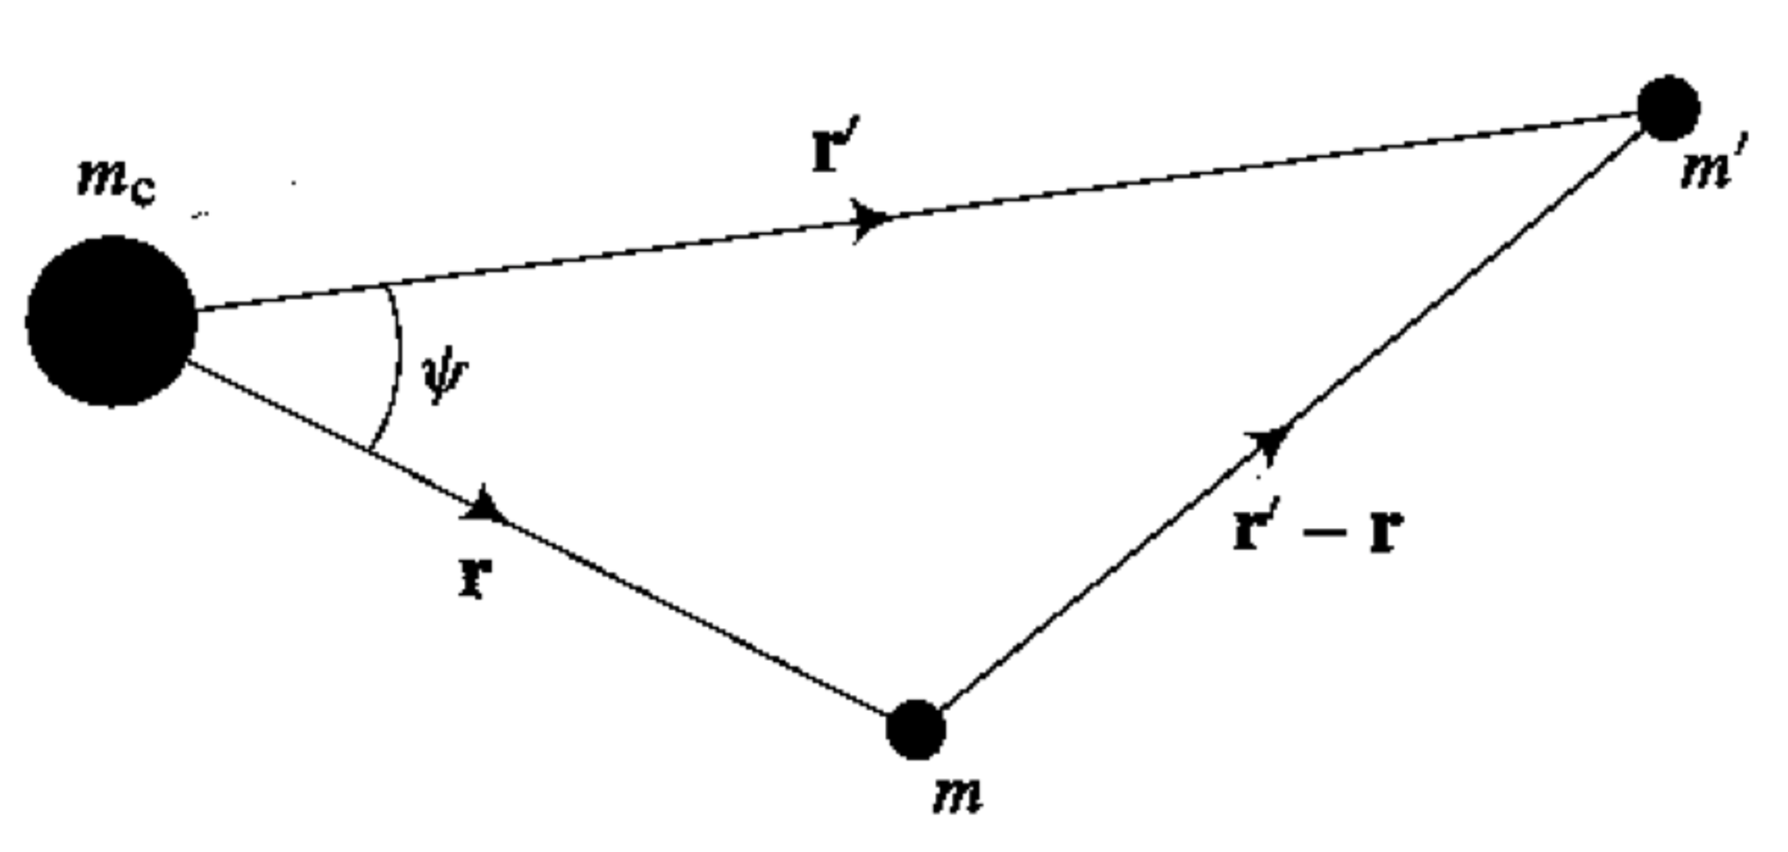
\includegraphics[width=10cm]{./image/sec6_2.pdf}
\caption{\label{}}
\end{figure}


\begin{figure}[H]
\centering
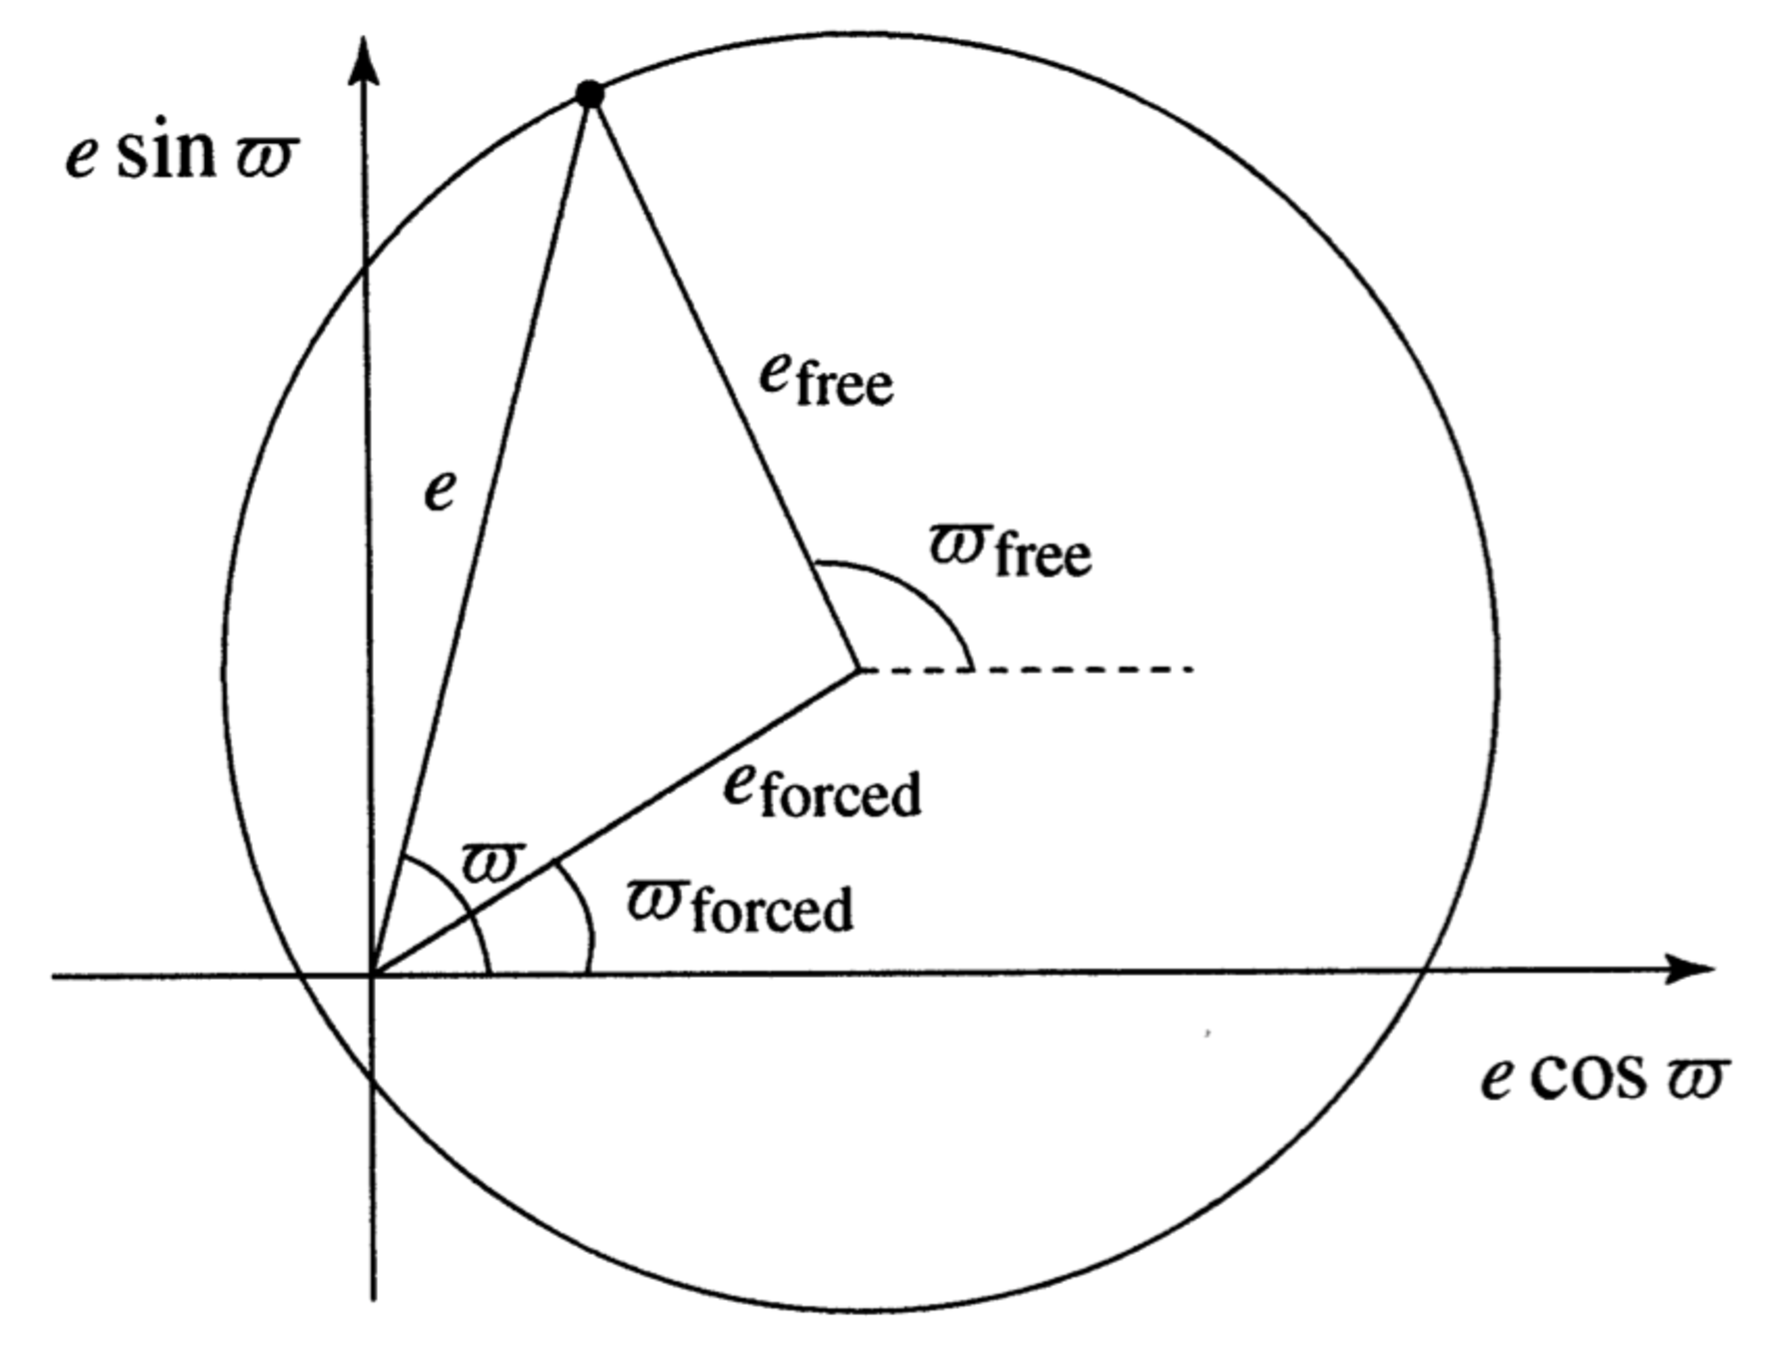
\includegraphics[width=10cm]{./image/sec7_2.pdf}
\caption{\label{}}
\end{figure}

\begin{figure}[H]
\centering
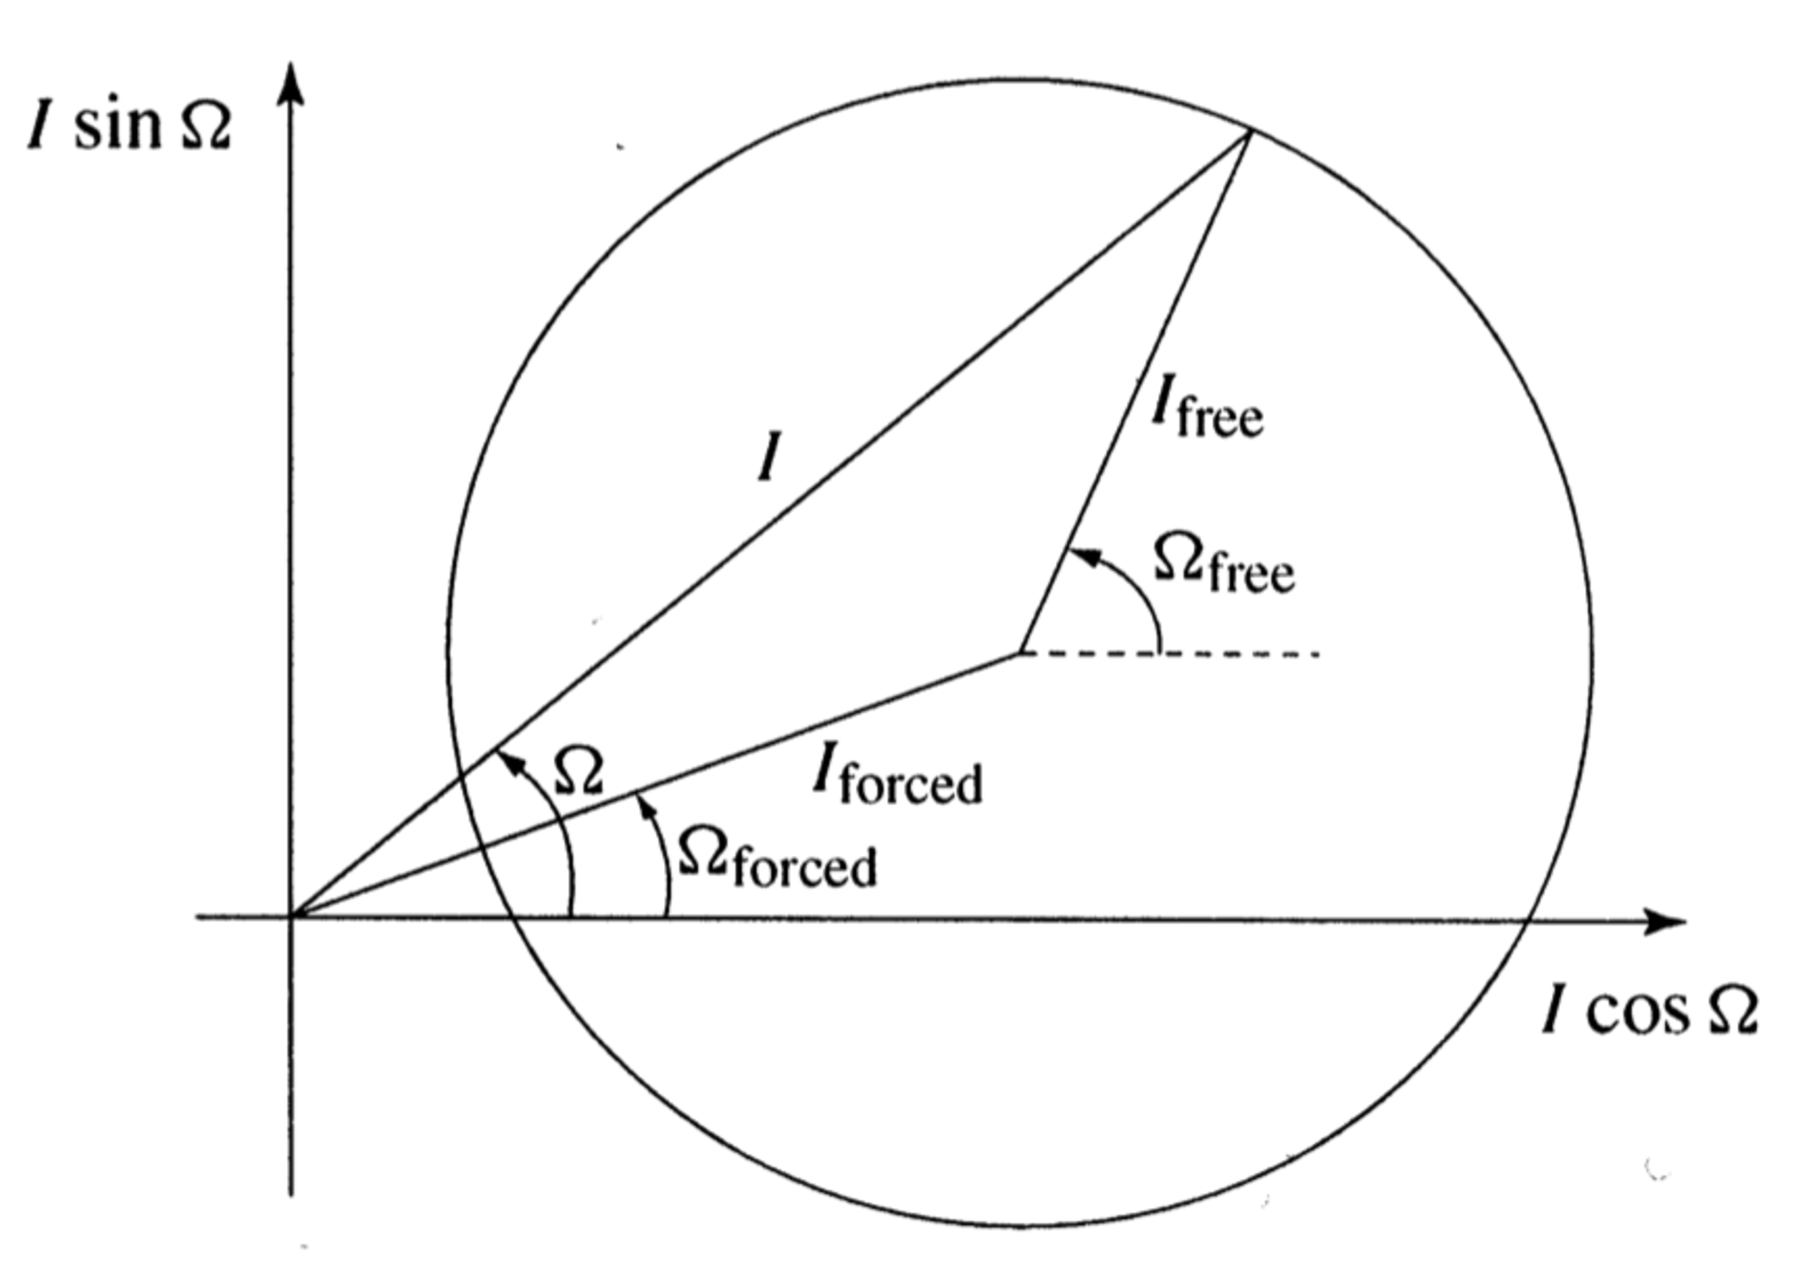
\includegraphics[width=10cm]{./image/sec7_3.pdf}
\caption{\label{}}
\end{figure}

\section{手法}
\subsection{4次のエルミート法 \label{sec:Hermite}}
\subsubsection{手順}
\begin{enumerate}
\item t での${\bm x}_j (t)$, ${\bm v}_j (t)$ ($\to {\bm x}_{0,j} , {\bm v}_{0,j}$) と加速度 ${\bm a}_j (t)$ ($\to {\bm a}_{0,j}$) とその時間微分 $\dot{{\bm a}}_j (t)$ ($\to \dot{{\bm a}}_{0,j}$) から,$t + \Delta t$ における位置と速度 (${\bm x}_{p,j} , {\bm v}_{p,j}$) を予測する.これらを予測子 (predictor) と呼ぶ.
\item 予測子を使って,加速度 ${\bm a}_{1,j}$ とその時間微分 $\dot{{\bm a}}_{1,j}$ を求める.
\item 修正子 : 必要な回数だけ (a),(b),(c) を繰り返す.
\begin{description}
\item[(a)] ${\bm a}_{0,j}$, $\dot{{\bm a}}_{0,j}$ と ${\bm a}_{1,j}$, $\dot{{\bm a}}_{1,j}$ から加速度の2階微分と3階微分 (${\bm a}_{0,j}^{(2)}$, ${\bm a}_{0,j}^{(3)}$) を計算する.
\item[(b)] ${\bm a}_{0,j}^{(2)}$, ${\bm a}_{0,j}^{(3)}$ を使い,予測子を修正する (${\bm x}_{c,j} , {\bm v}_{c,j}$).これらを修正子 (corrector) と呼ぶ.
\item[(c)] ${\bm x}_{c,j} , {\bm v}_{c,j}$ での加速度 (${\bm a}_{1,j}^{{\rm new}}$) とその時間微分 ($\dot{{\bm a}}_{1,j}^{{\rm new}}$) を計算し,(a) に戻る.
\end{description}
\item 次のステップの準備をする.3. のループの最後の ${\bm a}_{1,j}^{{\rm new}}$, $\dot{{\bm a}}_{1,j}^{{\rm new}}$ を次のステップのための ${\bm a}_{0,j}$ と $\dot{{\bm a}}_{0,j}$ に更新し,次のステップの $\Delta t$ を求める.1. に戻る.
\end{enumerate}

\subsubsection{予測子を求める \label{sec:predictor}}
$t + \Delta t$ での粒子の位置,速度を次のように予測する.
\begin{eqnarray}
{\bm x}_{p,j} & = & {\bm x}_{0,j} + \Delta t {\bm v}_{0,j} + \frac{\Delta t ^2}{2} {\bm a}_{0,j} + \frac{\Delta t ^3}{6} \dot{{\bm a}}_{0,j}, \\
{\bm v}_{p,j} & = & {\bm v}_{0,j} + \Delta t {\bm a}_{0,j} + \frac{\Delta t ^2}{2} \dot{{\bm a}}_{0,j}. 
\end{eqnarray}

$\Delta t$ に対して ${\bm x}_{p,j}$ は3次,${\bm v}_{p,j}$ は2次の精度.予測子全体の精度は2次なので,本来,${\bm x}_{p,j}$ も2次まででいいのだが,$\dot{{\bm a}}_{0,j}$ が与えられているので,3次まで付け加えておく.

\subsubsection{予測子から加速度と加速度の時間微分を求める}
${\bm x}_{p,j}, {\bm v}_{p,j}$ を使い,$t + \Delta t$ での加速度 ${\bm a}_{1,j}$ とその時間微分 $\dot{{\bm a}}_{1,j}$ は以下のように計算される.
\begin{eqnarray}
{\bm a}_{1,j} & = & - \sum_{k \not= j} G m_k \frac{{\bm r}_{jk}}{(r_{jk}^2 + \epsilon^2)^{3/2}}, \label{eq:a1j}\\
\dot{{\bm a}}_{1,j} & = & - \sum_{j} G m_k \left[ \frac{{\bm v}_{jk}}{(r_{jk}^2 + \epsilon^2)^{3/2}} - \frac{3 ( {\bm v}_{jk} \cdot {\bm r}_{jk} ) {\bm r}_{jk} }{(r_{jk}^2 + \epsilon^2)^{5/2}} \right]. \label{eq:a2j}
\end{eqnarray}

ここで,
\begin{eqnarray}
{\bm r}_{jk} & = & {\bm x}_{p,j} - {\bm x}_{p,k}, \\
{\bm v}_{jk} & = & {\bm v}_{p,j} - {\bm v}_{p,k}. 
\end{eqnarray}

$\epsilon$ は計算上の発散を抑えるための softning parameter で,近接相互作用について必要な計算精度に応じてとる.

${\bm a}_{1,j}$ は3次精度,$\dot{{\bm a}}_{1,j}$ は2次精度である.

\subsubsection{${\bm a}^{(2)}, {\bm a}^{(3)}$ を求める.\label{sec:corrector}}
Taylor 展開により,
\begin{eqnarray}
{\bm a}_{1,j} & = & {\bm a}_{0,j} + \Delta t \dot{{\bm a}}_{0,j} + \frac{\Delta t ^2}{2} {\bm a}_{0,j}^{(2)} + \frac{\Delta t ^3}{6} {\bm a}_{0,j}^{(3)}, \\
\dot{{\bm a}}_{1,j} & = & \dot{{\bm a}}_{0,j} + \Delta t {\bm a}_{0,j}^{(2)} + \frac{\Delta t ^2}{2} {\bm a}_{0,j}^{(3)}. 
\end{eqnarray}
なので,この2式を逆に解くと,
\begin{eqnarray}
{\bm a}_{0,j}^{(2)} & = & \frac{- 6 ({\bm a}_{0,j} - {\bm a}_{1,j}) - \Delta t (4 \dot{{\bm a}}_{0,j} + 2 \dot{{\bm a}}_{1,j})}{\Delta t ^2}, \\
{\bm a}_{0,j}^{(3)} & = & \frac{12 ({\bm a}_{0,j} - {\bm a}_{1,j}) + 6 \Delta t (\dot{{\bm a}}_{0,j} + \dot{{\bm a}}_{1,j})}{\Delta t ^3}. 
\end{eqnarray}
を得る.

\subsubsection{予測子の修正}
この ${\bm a}_{0,j}^{(2)}, {\bm a}_{0,j}^{(3)}$ を使って,位置と速度の予測子 (${\bm x}_{p,j}, {\bm v}_{p,j}$) を以下のように修正する.
\begin{eqnarray}
{\bm x}_{c,j} (t + \Delta t) & = & {\bm x}_{p,j} (t + \Delta t) +  \frac{\Delta t ^4}{24} {\bm a}_{0,j}^{(2)} + \alpha \frac{\Delta t ^5}{120} {\bm a}_{0,j}^{(3)}, \\
{\bm v}_{c,j} (t \Delta t) & = & {\bm v}_{p,j} (t +\Delta t) + \frac{\Delta t ^3}{6} {\bm a}_{0,j}^{(2)} + \frac{\Delta t ^4}{24} {\bm a}_{0,j}^{(3)}. 
\end{eqnarray}
ここで,普通にTaylor 展開を考えれば,$\alpha = 1$.ただし,$\alpha \not= 1$ とすることもある.この修正により,$\Delta t$ に対して,${\bm x}_j$ は5次,${\bm v}_j$ は4次の精度になる.積分全体の精度は4次.(${\bm a}_{0,j}^{(3)}$ が与えられているので,${\bm x}_j$ は5次まで書いておくが,係数には自由度がある.)

\subsubsection{修正された予測子を使って加速度および加速度の時間
微分を求める}
${\bm x}_{c,j}, {\bm v}_{c,j}$ での加速度 (${\bm a}_{1,j}^{\rm new}$) とその時間微分 ($\dot{{\bm a}}_{1,j}^{\rm new}$) を計算する.これらは,式 (\ref{eq:a1j}), (\ref{eq:a2j}) で,
\begin{eqnarray}
{\bm r}_{jk} & = & {\bm x}_{c,j} - {\bm x}_{c,k}, \\
{\bm v}_{jk} & = & {\bm v}_{c,j} - {\bm v}_{c,k}. 
\end{eqnarray}
とすれば求まる.

${\bm a}_{1,j}^{\rm new}, \dot{{\bm a}}_{1,j}^{\rm new}$ を ${\bm a}_{1,j}, \dot{{\bm a}}_{1,j}$ として,\ref{sec:corrector} に戻る.必要な回数だけこれを繰り返す (iteration).このループでは ${\bm x}_{p,j}, {\bm v}_{p,j}$ は更新しないことに注意.

\subsubsection{次のステップの準備}
ループが終わったら,最後の ${\bm a}_{1,j}^{\rm new}, \dot{{\bm a}}_{1,j}^{\rm new}$ を次のステップのための ${\bm a}_{0,j}, \dot{{\bm a}}_{0,j}$ に更新する.

\ref{sec:timestep} でも述べるが,次のステップの $\Delta t$ は,
\begin{equation}
\Delta t_j = \eta \sqrt{\frac{| {\bm a}_{1,j} | | {\bm a}_{1,j}^{(2)} | + | \dot{{\bm a}}_{1,j} | ^2}{| \dot{{\bm a}}_{1,j} | | {\bm a}_{1,j}^{(3)} | + | {\bm a}_{1,j}^{(2)} | ^2}}.
\end{equation}
で与えることが多い.$\eta$ は積分の精度を決めるパラメータで,1より小さな数で与える (例えば,$\eta = 0.01 - 0.05$).$\eta$ を小さくすると積分精度が良くなるが,計算は遅くなる.必要な精度を満たすようになるべく小さく,一方,計算時間が長くならないようになるべく大きく,という観点で最適な $\eta$ を選ぶ.

加速度の2階微分 (${\bm a}_{1,j}^{(2)}$) と 3階微分 (${\bm a}_{1,j}^{(3)}$) は,
\begin{eqnarray}
{\bm a}_{1,j}^{(3)} & = & {\bm a}_{0,j}^{(3)}, \\
{\bm a}_{1,j}^{(2)} & = & {\bm a}_{0,j}^{(2)} + {\bm a}_{0,j}^{(3)} \Delta t. 
\end{eqnarray}
のように見積もる.これは3次の精度で正しい.(Indiividual timestep ではこのまま進み,Shared timestep では $\Delta t_j$ で最小のものを $\Delta t$ とする.(\ref{sec:timestep} 参照))

そして,\ref{sec:predictor} に戻る.

$t = 0$ では,加速度の2階微分と3階微分は計算できないので,${\bm x}_j,{\bm v}_j$ での加速度 (${\bm a}_{0,j}$) とその時間微分を求め,
\begin{equation}
\Delta t_j = \eta \frac{|{\bm a}_j|}{|\dot{{\bm a}}_j|}.
\end{equation}
のようにしてから,\ref{sec:predictor} に戻る.

\subsection{中心星重力}
中心星の周りに微惑星が回っている場合,中心星重力がほとんどの時間で圧倒的に大きい場合が多いので,中心星重力を別にして計算することが多い.簡単のため,中心星 ($j = 0$) とその周りを回る2つの天体 ($j = 1, 2$) の3体問題を考える.3天体の重心を原点にとった座標系 (慣性系) での運動方程式は,
\begin{eqnarray}
{\bm a}_0 & = & G m_1 \frac{{\bm r}_1 - {\bm r}_0}{|{\bm r}_1 - {\bm r}_0|^3} + G m_2  \frac{{\bm r}_2 - {\bm r}_0}{|{\bm r}_2 - {\bm r}_0|^3}, \label{eq:a0}\\
{\bm a}_1 & = & G m_0 \frac{{\bm r}_0 - {\bm r}_1}{|{\bm r}_10- {\bm r}_1|^3} + G m_2  \frac{{\bm r}_2 - {\bm r}_1}{|{\bm r}_2 - {\bm r}_1|^3}, \label{eq:a1}\\
{\bm a}_2 & = & G m_0 \frac{{\bm r}_0 - {\bm r}_2}{|{\bm r}_0 - {\bm r}_2|^3} + G m_1  \frac{{\bm r}_1 - {\bm r}_2}{|{\bm r}_1 - {\bm 2}_0|^3}. \label{eq:a2}
\end{eqnarray}

中心星を中心とした運動方程式を作る.式 (\ref{eq:a1}), (\ref{eq:a2}) から (\ref{eq:a0}) を辺々引くと,
\begin{eqnarray}
{\bm a}_1 & = & G (m_0 + m_1) \frac{{\bm r}_1}{|{\bm r}_1|^3} + G m_2 \frac{{\bm r}_1 - {\bm r}_2}{|{\bm r}_1 - {\bm r}_2|^3} - G m_2 \frac{{\bm r}_2}{|{\bm r}_2|^3}, \\
{\bm a}_2 & = & G (m_0 + m_2) \frac{{\bm r}_2}{|{\bm r}_2|^3} + G m_1 \frac{{\bm r}_2 - {\bm r}_1}{|{\bm r}_2 - {\bm r}_1|^3} - G m_1 \frac{{\bm r}_1}{|{\bm r}_1|^3}. 
\end{eqnarray}
それぞれの式の第1項が中心星からの重力,第2項が相互作用,第3項が indirect 項となっている.これらの時間微分は,
\begin{eqnarray}
\begin{split}
\dot{{\bm a}}_1 = & - G (m_0 + m_1) \left[ \frac{{\bm v}_1}{|{\bm r}_1|^3} - 3 \frac{({\bm v}_1 \cdot {\bm r}_1) {\bm r}_1}{|{\bm r}_1|^5} \right] \\
& - G m_2 \left[ \frac{{\bm v}_1 - {\bm v}_2}{|{\bm r}_1 - {\bm r}_2|^3} - 3 \frac{[({\bm v}_1 - {\bm v}_2) \cdot ({\bm r}_1 - {\bm r}_2)] ({\bm r}_1 - {\bm r}_2)}{|{\bm r}_1 - {\bm r}_2|^5} \right] \\
& - G m_2 \left[ \frac{{\bm v}_2}{|{\bm r}_2|^3} - 3 \frac{{\bm v}_2 \cdot {\bm r}_2}{|{\bm r}_2|^5} {\bm r}_2 \right], 
\end{split}
\\
\begin{split}
\dot{{\bm a}}_2 = & - G (m_0 + m_2) \left[ \frac{{\bm v}_2}{|{\bm r}_2|^3} - 3 \frac{({\bm v}_2 \cdot {\bm r}_2) {\bm r}_2}{|{\bm r}_2|^5} \right] \\
& - G m_1 \left[ \frac{{\bm v}_2 - {\bm v}_1}{|{\bm r}_2 - {\bm r}_1|^3} - 3 \frac{[({\bm v}_2 - {\bm v}_1) \cdot ({\bm r}_2 - {\bm r}_1)] ({\bm r}_2 - {\bm r}_1)}{|{\bm r}_2 - {\bm r}_1|^5} \right] \\
& - G m_1 \left[ \frac{{\bm v}_1}{|{\bm r}_1|^3} - 3 \frac{{\bm v}_1 \cdot {\bm r}_1}{|{\bm r}_1|^5} {\bm r}_1 \right].
\end{split}
\end{eqnarray}
第1項,第2項,第3項は,加速度のそれぞれの項の時間微分に対応している.

N 体問題の場合に拡張して考えると,$i, j = 1, 2, 3, \cdots, N$ に対して,
\begin{eqnarray}
{\bm a}_i & = & - G m_0 \frac{{\bm r}_i}{|{\bm r}_i|^3}  + \sum_{j \not= i} G m_j \frac{{\bm r}_{ij}}{|{\bm r}_{ij} |^3} - \sum_j G m_j \frac{{\bm r}_j}{|{\bm r}_j|^3}, \label{eq:ai} \\
\dot{{\bm a}}_j & = & - G m_0 \left[ \frac{{\bm v}_i}{|{\bm r}_i|^3} - 3 \frac{({\bm v}_i \cdot {\bm r}_i) {\bm r}_i}{|{\bm r}_i|^5} \right] \nonumber \\ 
& & - \sum_{j \not= i} G m_j \left[ \frac{{\bm v}_{ij}}{|{\bm r}_{ij}|^3} - 3 \frac{[{\bm v}_{ij} \cdot {\bm r}_{ij}] {\bm r}_{ij}}{|{\bm r}_{ij}|^5} \right] - \sum_j G m_j \left[ \frac{{\bm v}_j}{|{\bm r}_j|^3} - 3 \frac{{\bm v}_j \cdot {\bm r}_j}{|{\bm r}_j|^5} {\bm r}_j \right]. \label{eq:adoti}
\end{eqnarray}
となる.ここで,
\begin{eqnarray}
{\bm r}_{ij} & = & {\bm r}_{i} - {\bm r}_{j}, \\
{\bm v}_{ij} & = & {\bm v}_{i} - {\bm v}_{j}.
\end{eqnarray}
(\ref{eq:ai}), (\ref{eq:adoti}) 式の indirect 項は i にはよらないので,一度計算しておけば,全ての粒子 i に対して使えることに注意.

回っている天体の質量が中心星に対して非常に小さい場合は,(\ref{eq:ai}), (\ref{eq:adoti}) 式の第3項の indirect 項は第1項の中心星重力項に比べて無視できる.そのようなときには第3項の indirect 項を落とし,中心星の動きは無視して,中心星重力は外場として扱うことも多い.
\begin{eqnarray}
{\bm a}_i & = & - G m_0 \frac{{\bm r}_i}{|{\bm r}_i|^3}  + \sum_{j \not= i} G m_j \frac{{\bm r}_{ij}}{|{\bm r}_{ij} |^3},  \\
\dot{{\bm a}}_j & = & - G m_0 \left[ \frac{{\bm v}_i}{|{\bm r}_i|^3} - 3 \frac{({\bm v}_i \cdot {\bm r}_i) {\bm r}_i}{|{\bm r}_i|^5} \right] - \sum_{j \not= i} G m_j \left[ \frac{{\bm v}_{ij}}{|{\bm r}_{ij}|^3} - 3 \frac{[{\bm v}_{ij} \cdot {\bm r}_{ij}] {\bm r}_{ij}}{|{\bm r}_{ij}|^5} \right].
\end{eqnarray}
このほうが計算コストはずっと軽くなる.

以下のテスト計算,本計算では,中心星重力を外場として扱うことにした.

\subsection{タイムステップ \label{sec:timestep}}
\subsubsection{Variable Timestep (可変タイムステップ) \label{sec:variable}}
軌道計算の $\Delta t$ が大きすぎると数値的な誤差が大きくなり,逆に小さすぎても計算コストがかかる.したがって,取り扱う問題やその時の状態に合った $\Delta t$ を選ぶ必要がある.特に,時々刻々と状態が大きく変化するような現象 (近接相互作用など) を取り扱う場合は,$\Delta t$ を可変にするべきである.

$\Delta t$ をどのように決めればよいかを考える.ある時刻 $t$ での粒子の位置を $x (t)$ とすると,$t + \Delta t$ での位置は,
\begin{equation}
x (t + \Delta t)  =  x (t) + v (t) \Delta t + \frac{1}{2!} a (t) (\Delta t)^2 + \cdots \label{eq:xt}
\end{equation}
と書ける.数値計算では (\ref{eq:xt}) 式の展開を有限項で打ち切ったものを使うため,精度の良い計算をするためには,$\Delta t$ が十分小さい必要がある.1次精度,2次精度のそれぞれの $\Delta t$ に関しての条件式が得られる.
\begin{eqnarray}
1次精度 : \Delta t & \ll & \frac{|x (t)|}{|v (t)|}, \label{eq:1storder} \\
2次精度 : \Delta t & \ll & {\rm min} \left( \frac{|x (t)|}{|v (t)|}, \frac{|v (t)|}{|a (t)|} \right). \label{eq:2ndorder}
\end{eqnarray}
$\Delta t$ は常に (\ref{eq:1storder}),(\ref{eq:2ndorder}) 式を満たすように決めなければならない.例えば,係数 $\eta (\ll 1)$ を用いて,時刻 $t$ での $\Delta t$ を
\begin{eqnarray}
1次精度 : \Delta t & = & \eta \frac{|x (t)|}{|v (t)|}, \label{eq:1storder} \\
2次精度 : \Delta t & = & \eta \frac{1}{\sqrt{\left( \frac{v (t)}{x (t)} \right)^2 + \left( \frac{a (t)}{v (t)} \right)^2}}. \label{eq:2ndorder}
\end{eqnarray}
ととればよい.

\ref{sec:Hermite} のエルミート法は4次精度である.${\bm x}, {\bm v}$ の6変数の4次の場合,上と同様に考えるとタイムステップの標識が繁雑になるので,もっと簡単な近似的な表式が用いられることが多い.よく用いられる表式は,
\begin{equation}
\Delta t  =  \eta \frac{|{\bm a}|}{|\dot{{\bm a}}|},
\end{equation}
または
\begin{equation}
\Delta t  =  \eta \sqrt{\frac{| {\bm a}| | {\bm a}^{(2)} | + | \dot{{\bm a}}| ^2}{| \dot{{\bm a}}| | {\bm a}^{(3)} | + | {\bm a}^{(2)} | ^2}} \label{eq:Aarseth}
\end{equation}
である.(\ref{eq:Aarseth}) 式は Aarseth によるもので,簡単でありながら非常に
効率がよいタイムステップの表式であることが知られている.

\subsubsection{Shared Timestep (共有タイムステップ) とその限界}
N 体計算では,各粒子 $j$ について,\ref{sec:variable} でやったようにして,$\Delta t_j (j = 1, 2, 3, \cdots , N)$ を計算する.例えば,その最小値
\begin{equation}
\Delta t  =  {\rm min} (\Delta t_j) ; j = 1, \cdots , N
\end{equation}
を全粒子の $\Delta t$ に採用して積分すれば,精度が保てる.このようなタイムステップの決め方を "shared timestep" と呼ぶ.

しかしながら,粒子同士の近接相互作用や衝突がしばしば起こり,その近接相互作用や衝突が重要なプロセスになる「衝突系」の場合 (惑星形成のシミュレーションや銀河や星団の準静的進化のシュミレーションはそういう場合に対応する) では,"shared timestep" では非常に効率が悪い.そこで考えだされたのが,以下に述べる "individual timestep" である.これは「力学的に本来必要な timestep」で切っていこうという方法である.

また,global な計算領域を持つ場合も事情は似ている.例えば水星領域から土星領域までを含む計算の場合,水星領域での太陽まわりのケプラー時間と土星領域でのそれは 100 倍も異なる.近接相互作用をしていない粒子は太陽まわりのケプラー時間に比例した timestep で切ることになるので,"shared timestep" では水星領域でのケプラー時間を基準にして土星領域の計算をするので,効率が悪い.この場合も "individual timestep" が有効になる.

\subsubsection{Individual Timestep (独立タイムステップ) }
"individual timestep" では,粒子は各々別の時間 $t_j$を持ち,別々に時間発展していく.計の時間 ("system time" または "global time") は $t_j + \Delta t_j$ が最小になる粒子 (進めた先が一番遅れている粒子) と共に進んでいく.

粒子は各々別の時間 $t_j$ での位置 ${\bm x}_j (t_j)$,速度 ${\bm v}_j (t_j)$,加速度 ${\bm a}_j (t_j)$,加速度の時間微分 $\dot{{\bm a}}_j (t_j)$ の情報を持っていて,ある与えられた精度 ($\eta$) で次に進むことができる timestep $\Delta t_j$ が計算されているとする.

\begin{enumerate}
\item $t_j + \Delta t_j$ が最小となる粒子 $j_{{\rm sys}}$ を選び,その時間を system time $t_{{\rm sys}}$ とする.
\item $t_{{\rm sys}}$ における全ての粒子の予測子を計算する.
\item 予測子を使って,$t_{{\rm sys}}$ での $j_{{\rm sys}}$ 粒子の ${\bm a}_{j_{{\rm sys}}}(t_{j_{{\rm sys}}}), \dot{{\bm a}}_{j_{{\rm sys}}} (t_{j_{{\rm sys}}})$ を計算する.
\item $j_{{\rm sys}}$ 粒子のみを修正する.iteration をする場合も $j_{{\rm sys}}$ 粒子以外は予測子を使う.
\item 新たな $\Delta t_{j_{{\rm sys}}}$  を計算し,$t_{j_{{\rm sys}}} + \Delta t_{j_{{\rm sys}}}$ を新たな $t_{j_{{\rm sys}}}$ として更新し,ステップ1に戻る.$j_{{\rm sys}}$ 粒子以外は予測子を捨ててもとに戻る.
\end{enumerate}

N 体計算で一番計算時間がかかるのが,$\mathcal{O} (N^2)$ の相互重力計算である.予測子はすでに持っている ${\bm x}_j (t_j), {\bm v}_j (t_j), {\bm a}_j (t_j), \dot{{\bm a}}_j (t_j)$ を使って,$t_{{\rm sys}} - t_j$ の時間分だけ予測すればいいので,$\mathcal{O} (N)$ の計算である.すなわち,進める (update する) 粒子がどんなに細かい $\Delta t_j$ でステップを切っていっても,他の粒子は実際上進むことはせず,"shared timestep" のときのように $\mathcal{O} (N^2)$ の無駄な計算を繰り返すことはない.このことにより,"individual timestep" を使うと計算が大幅に加速されることがわかる.

\section{重力散乱テスト計算}
\subsection{1体のケプラー運動 (エネルギー,角運動量とタイムステップの関係)}

\begin{figure}[H]
\centering
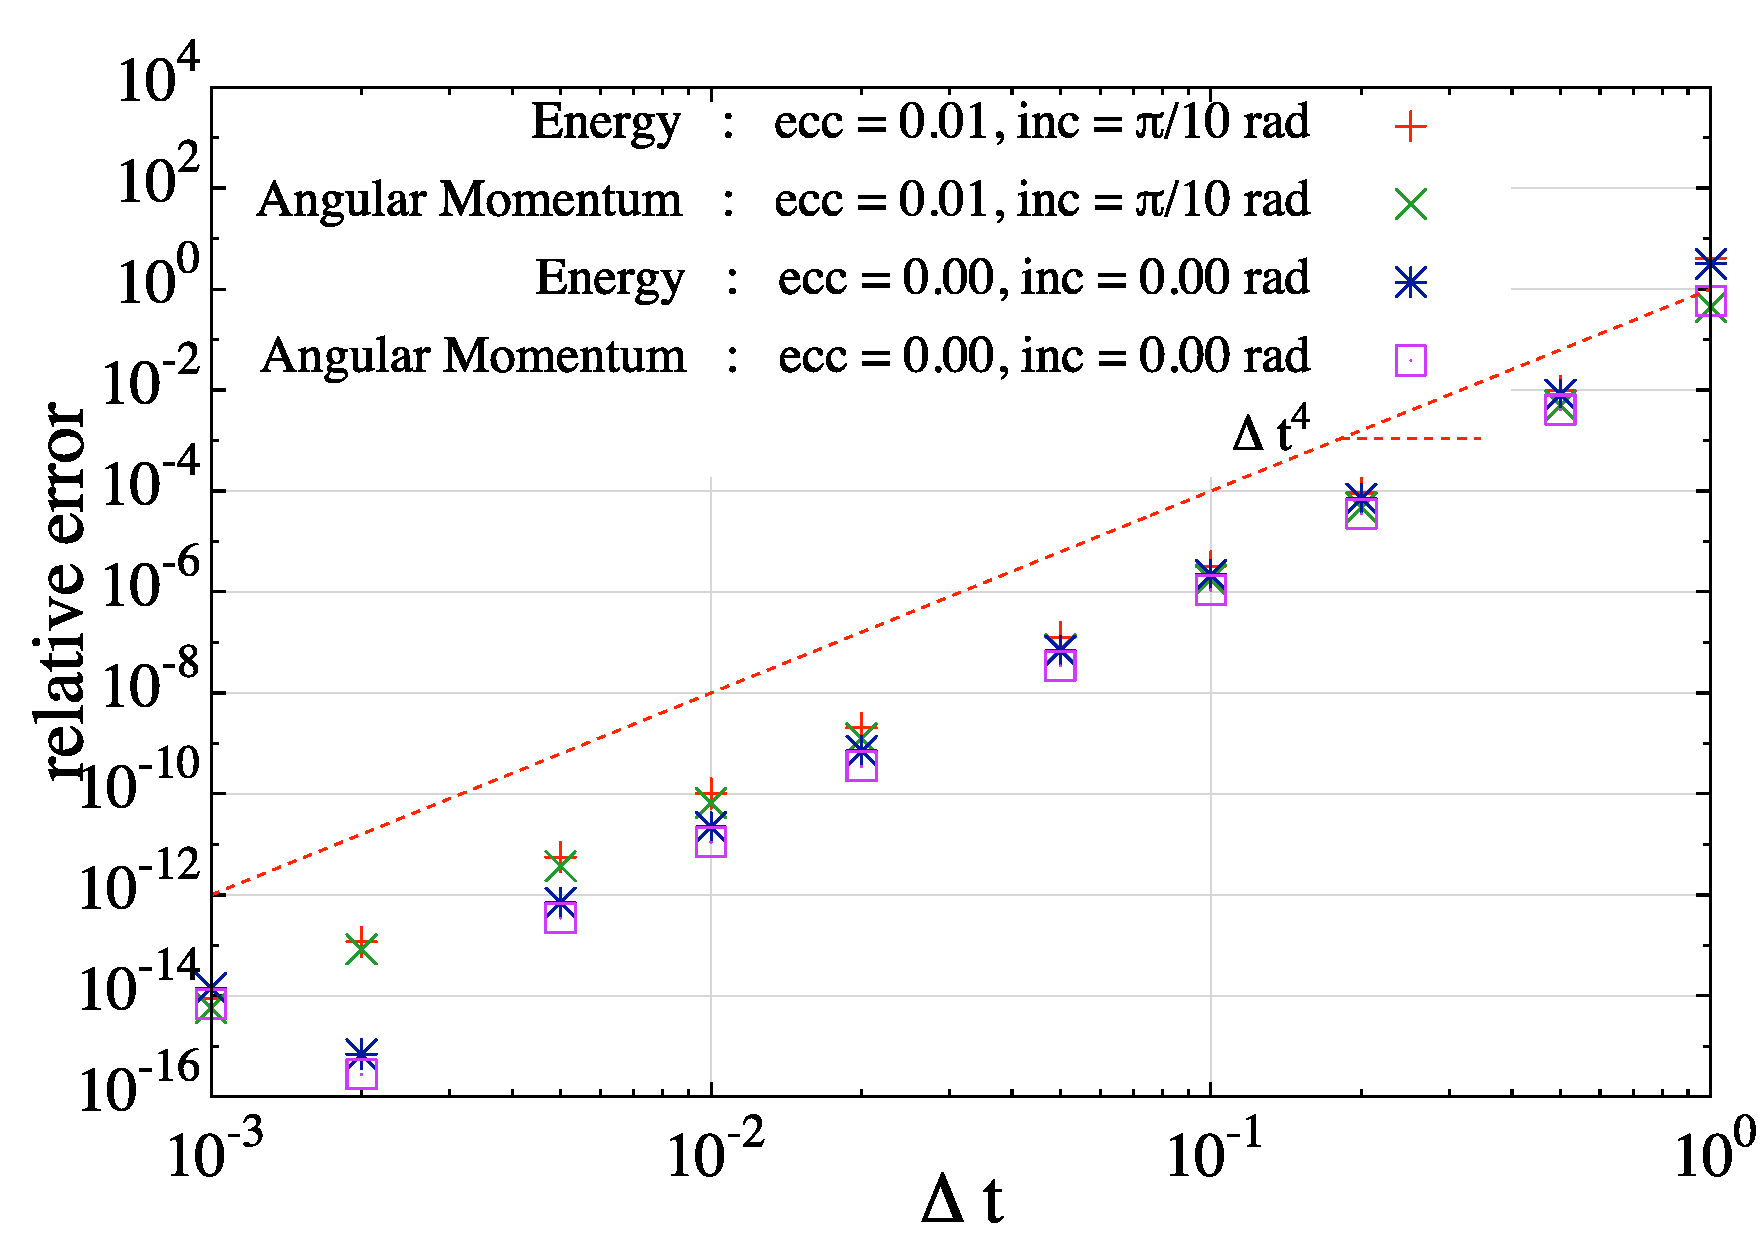
\includegraphics[width=10cm]{./image/relative_error.pdf}
\caption{\label{}}
\end{figure}

\subsection{円軌道の惑星と微惑星の重力散乱}

\begin{figure}[H]
\centering
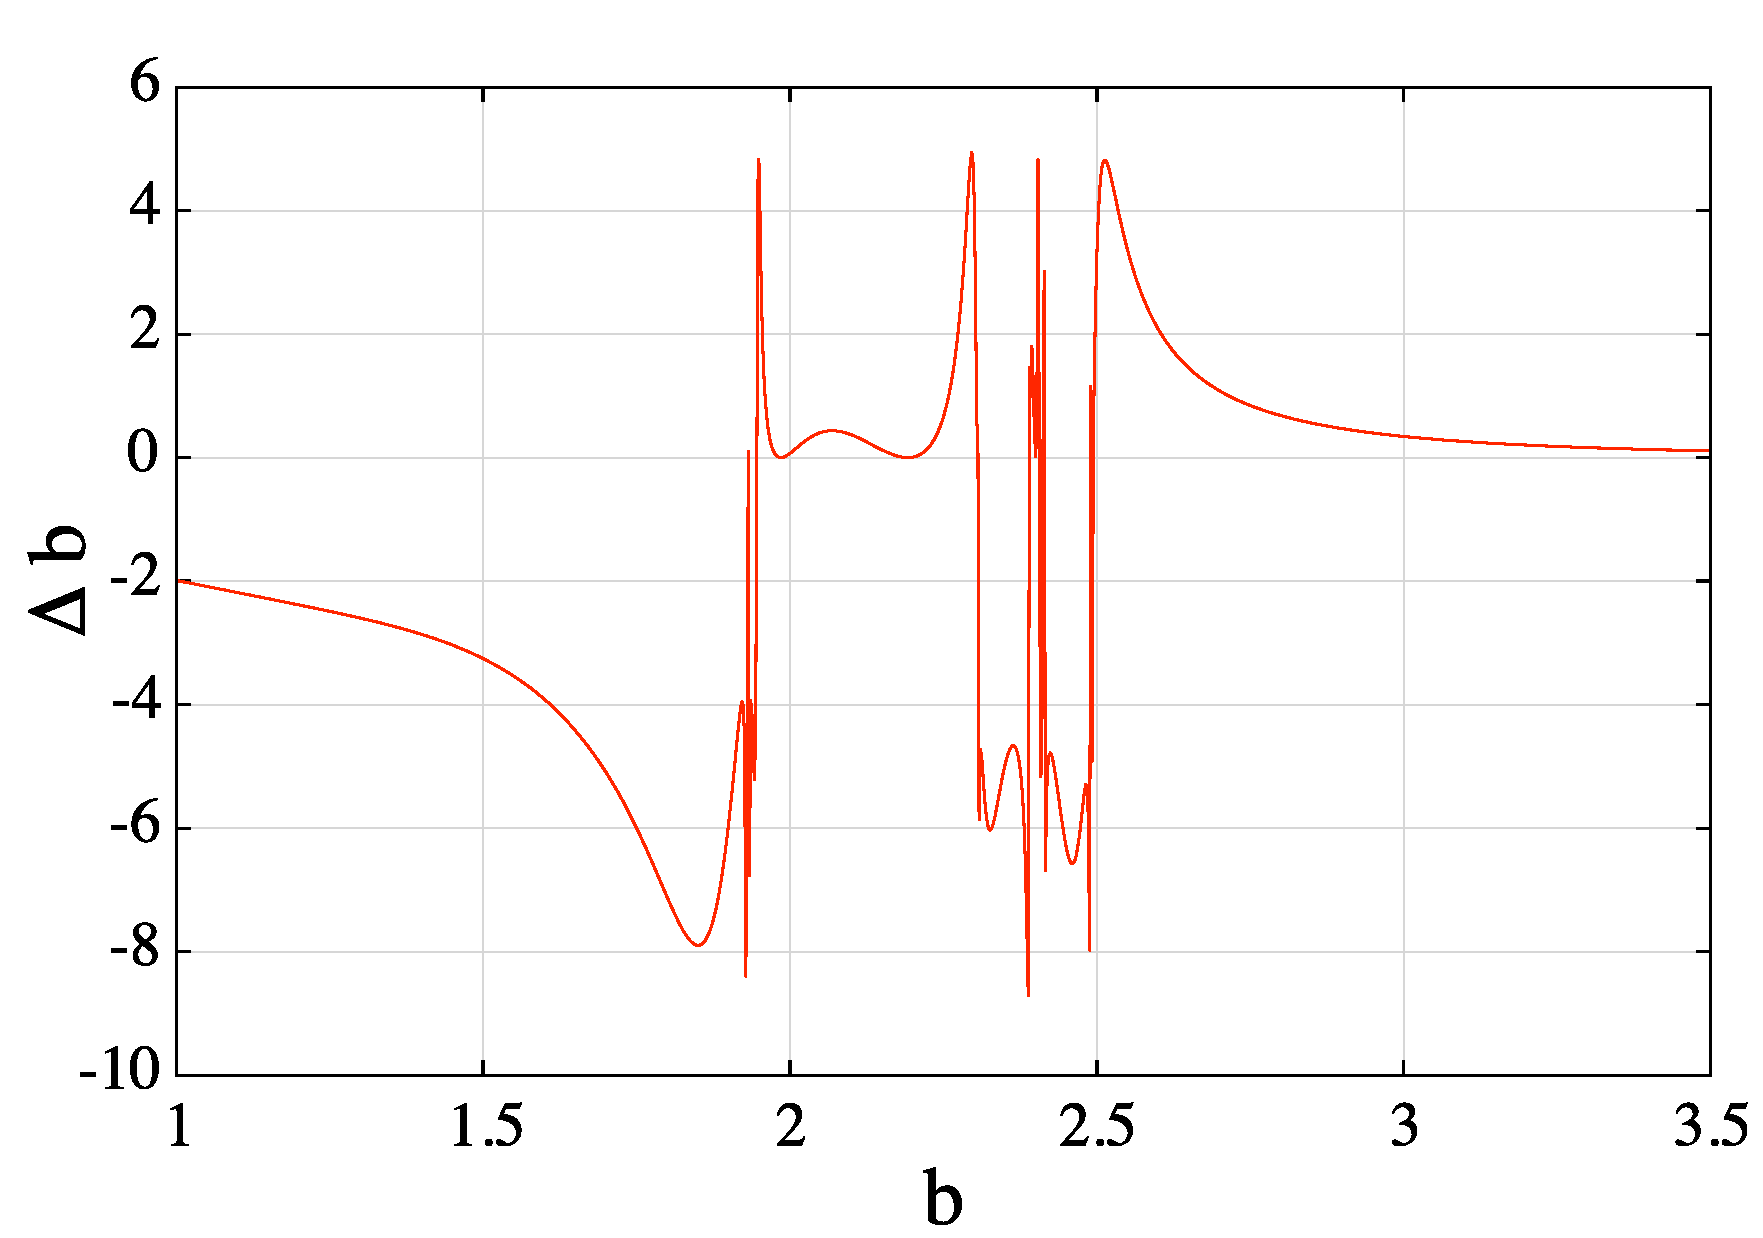
\includegraphics[width=10cm]{./image/planetesimal_delta_b.pdf}
\caption{\label{}}
\end{figure}

\begin{figure}[H]
\centering
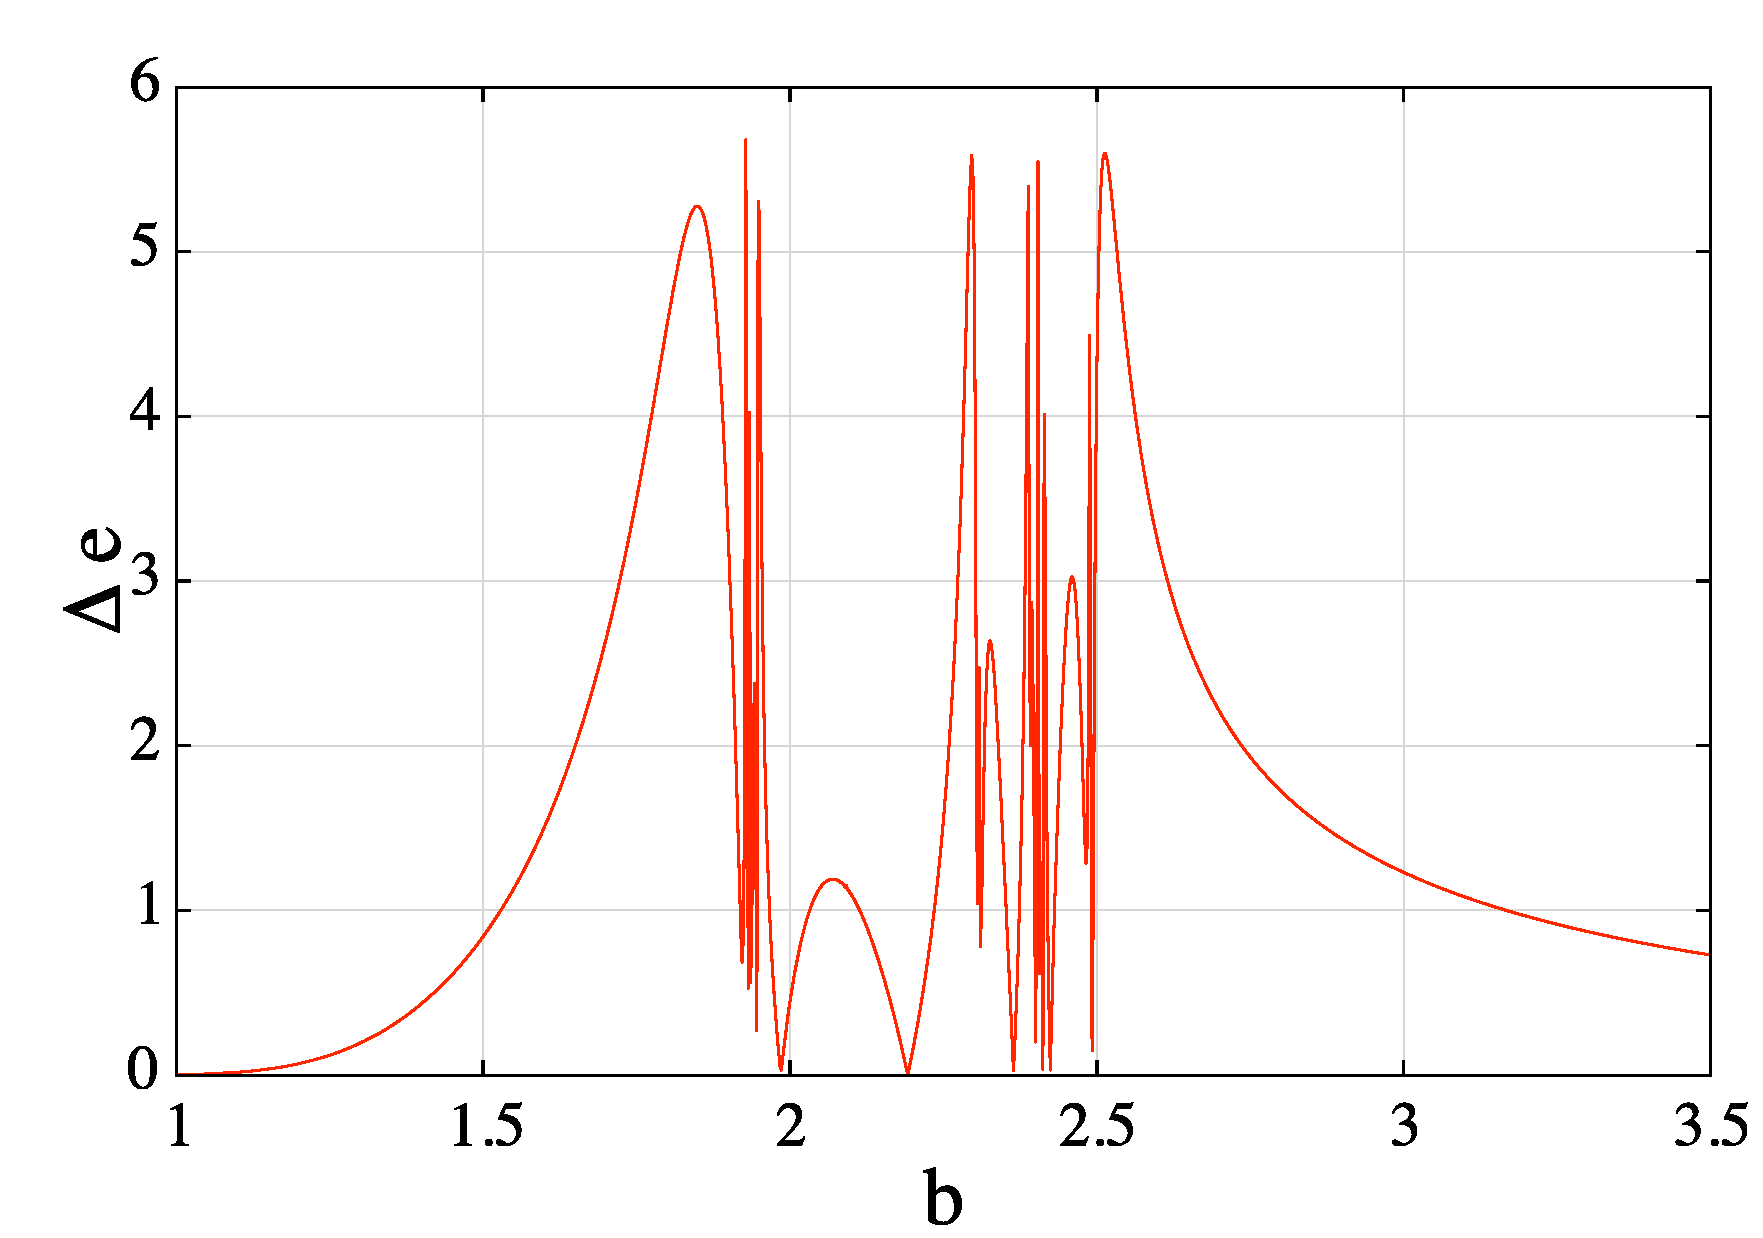
\includegraphics[width=10cm]{./image/planetesimal_delta_e.pdf}
\caption{\label{}}
\end{figure}

\begin{figure}[H]
\centering
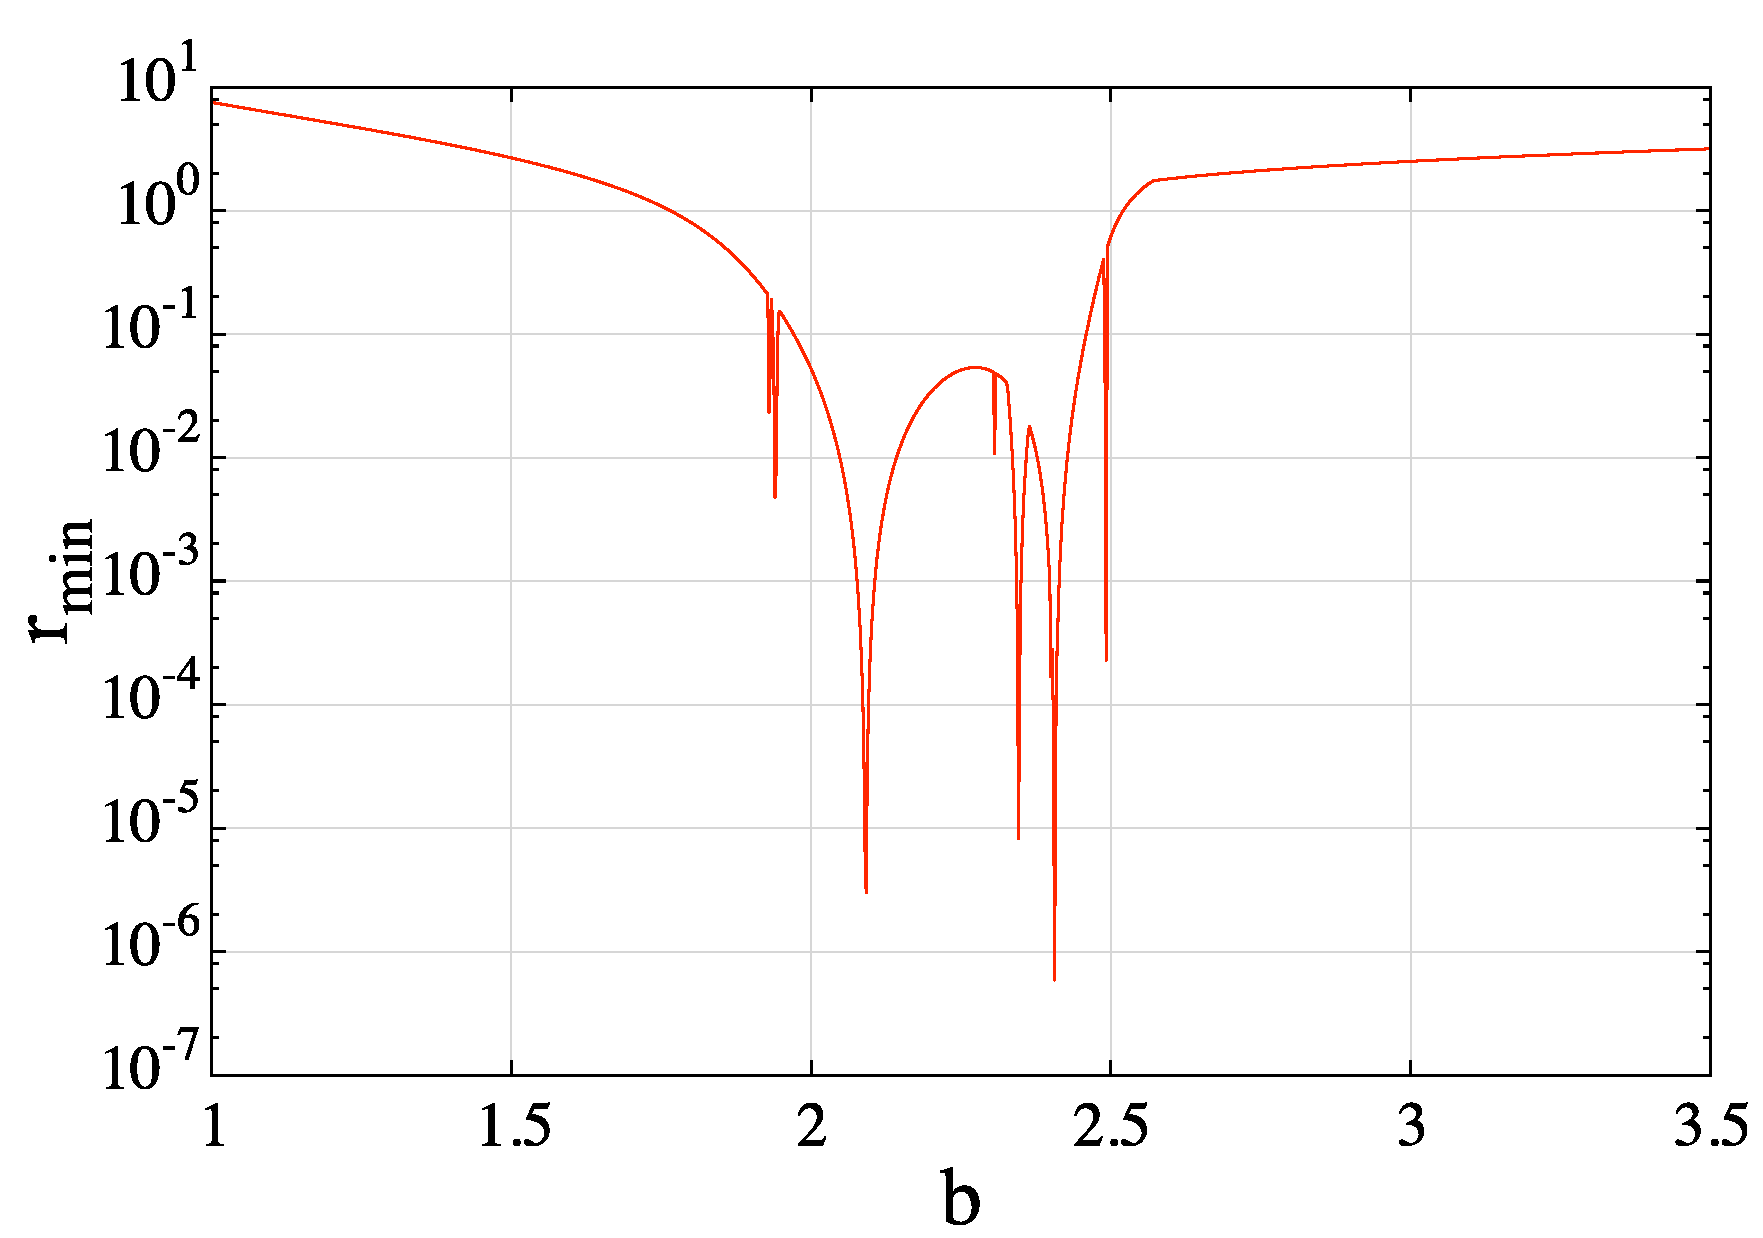
\includegraphics[width=10cm]{./image/planetesimal_r_min.pdf}
\caption{\label{}}
\end{figure}

\subsection{ピタゴラス問題}

\begin{figure}[H]
\centering
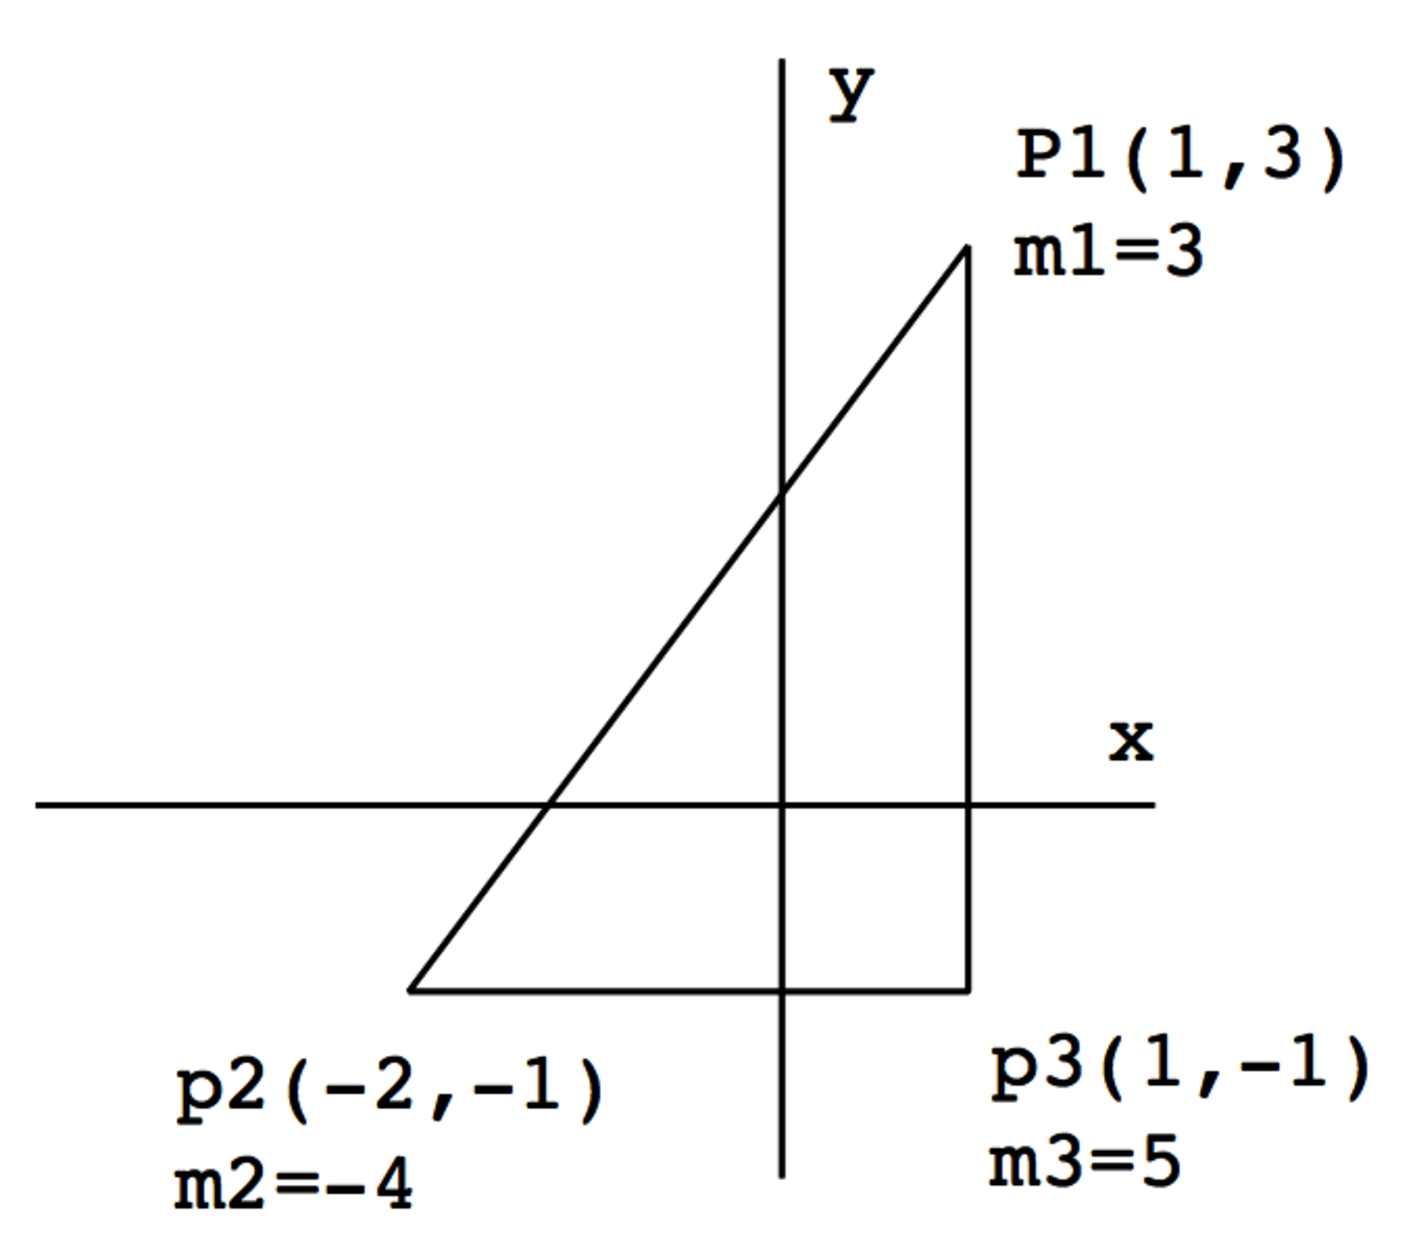
\includegraphics[width=10cm]{./image/pythagoras_1.pdf}
\caption{\label{}}
\end{figure}



\begin{figure}[H]
\begin{tabular}{cc}
%左
\begin{minipage}[t]{0.45\hsize}
\centering
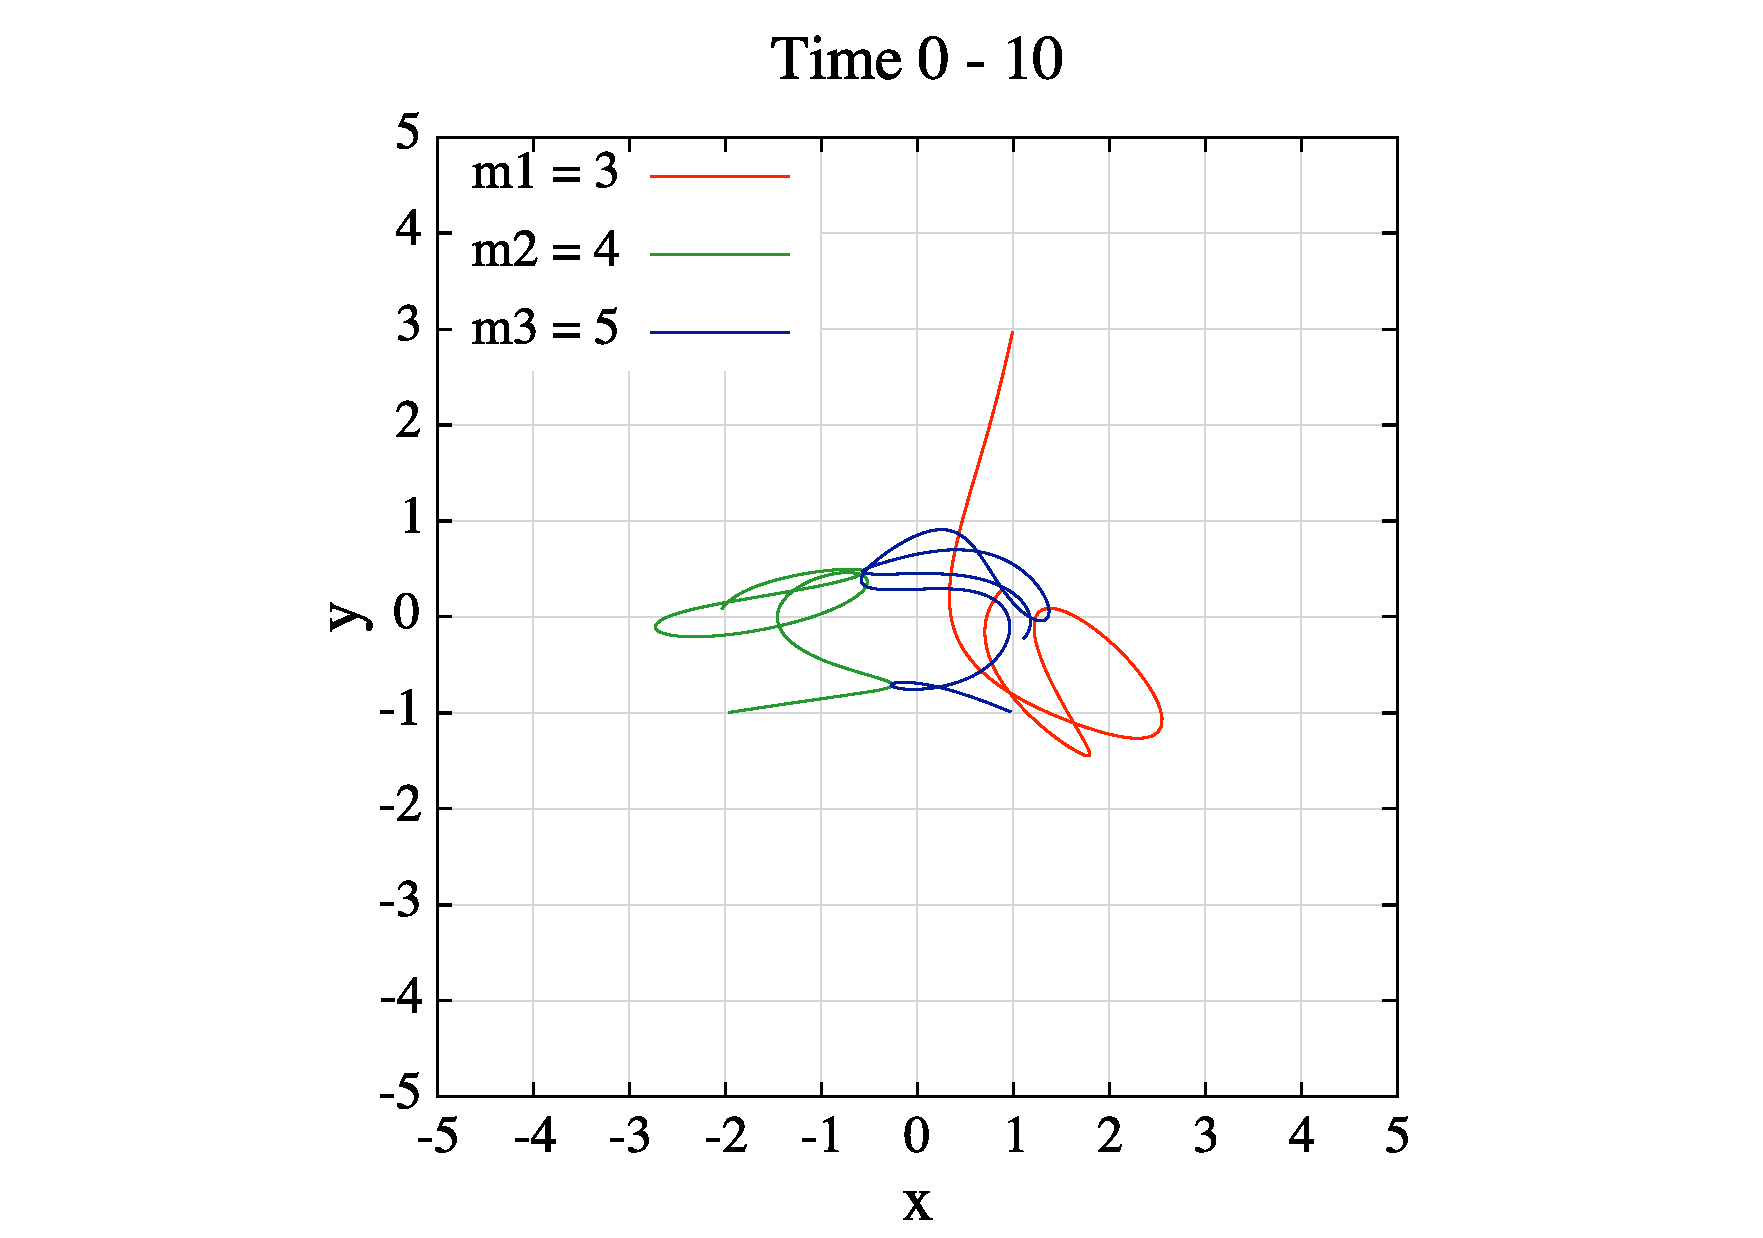
\includegraphics[width=8cm]{./image/pythagoras_orbit_0to10.pdf}
\end{minipage} &
%右
\begin{minipage}[t]{0.45\hsize}
\centering
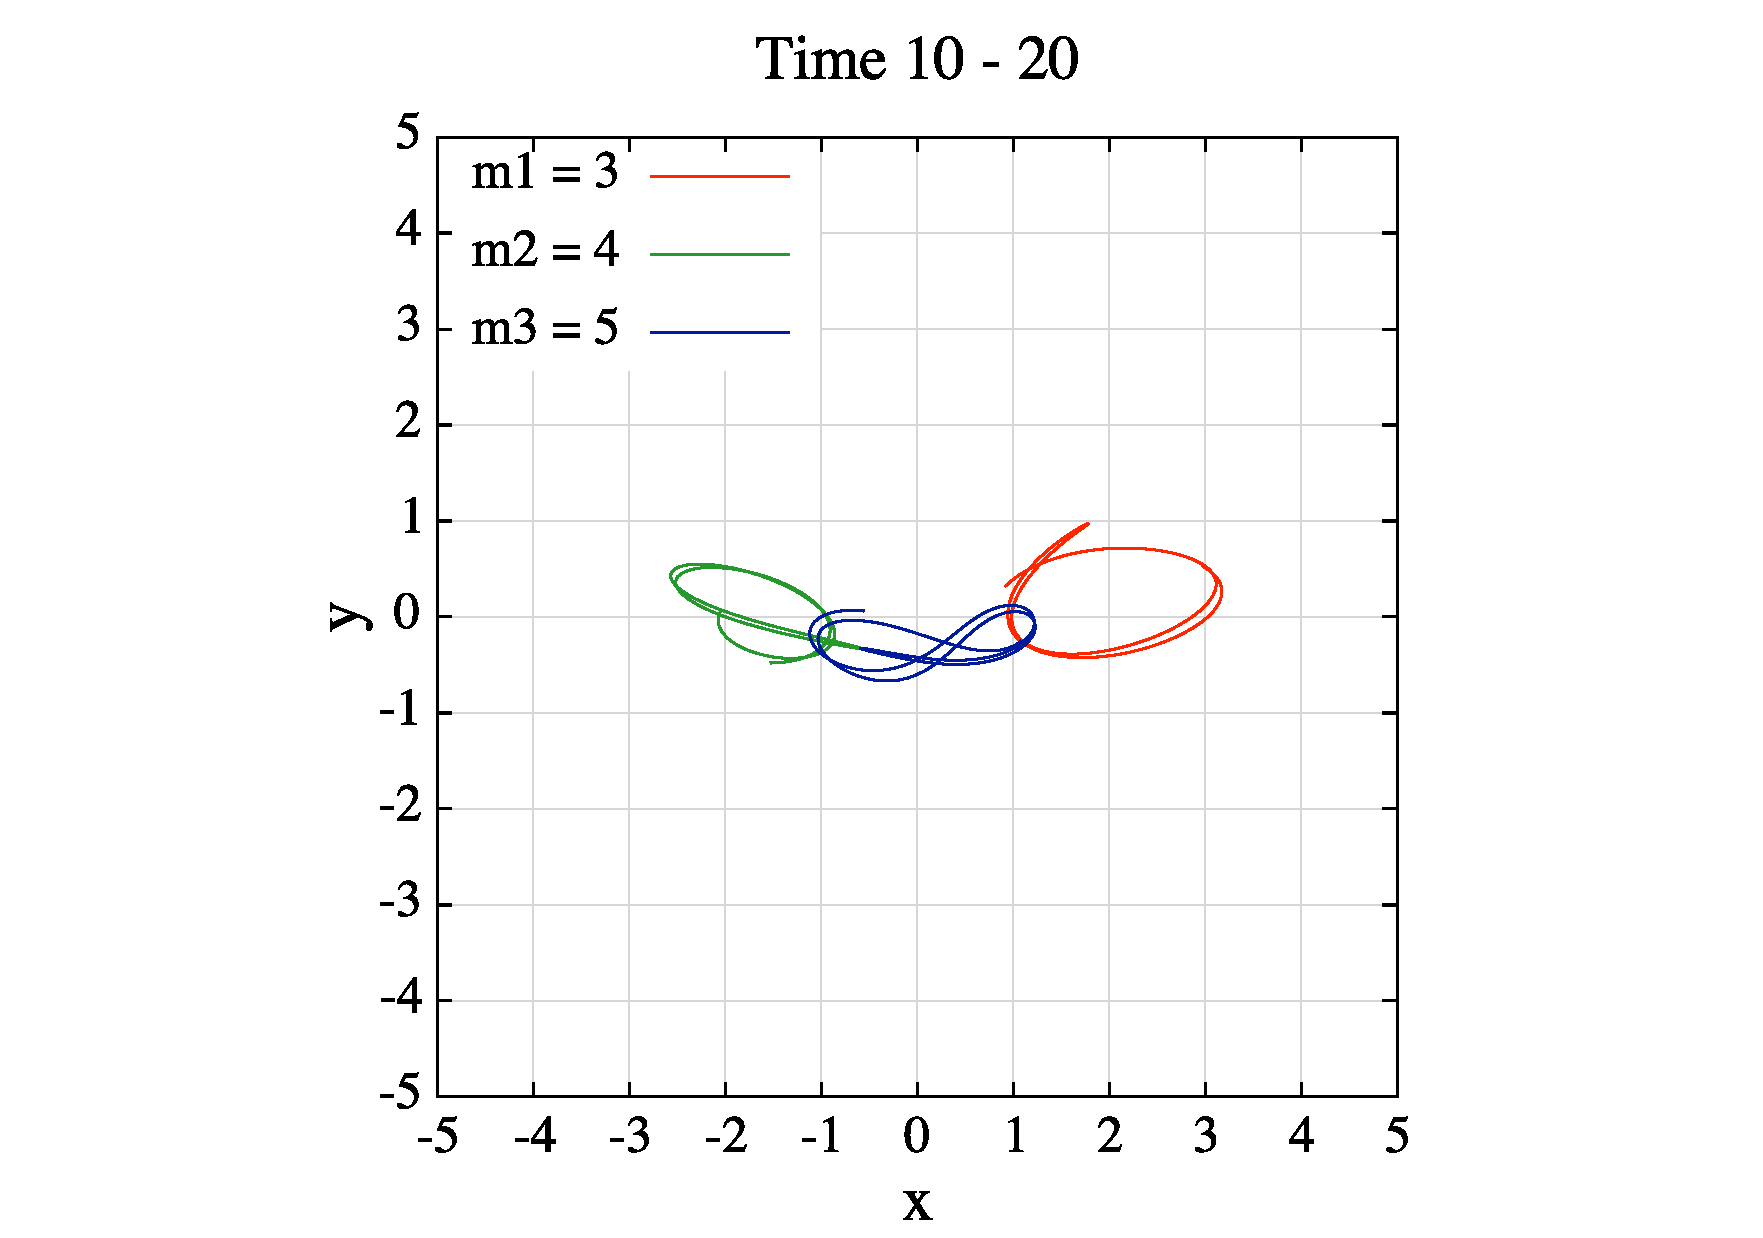
\includegraphics[width=8cm]{./image/pythagoras_orbit_10to20.pdf}
\end{minipage}\\
%
%左
\begin{minipage}[t]{0.45\hsize}
\centering
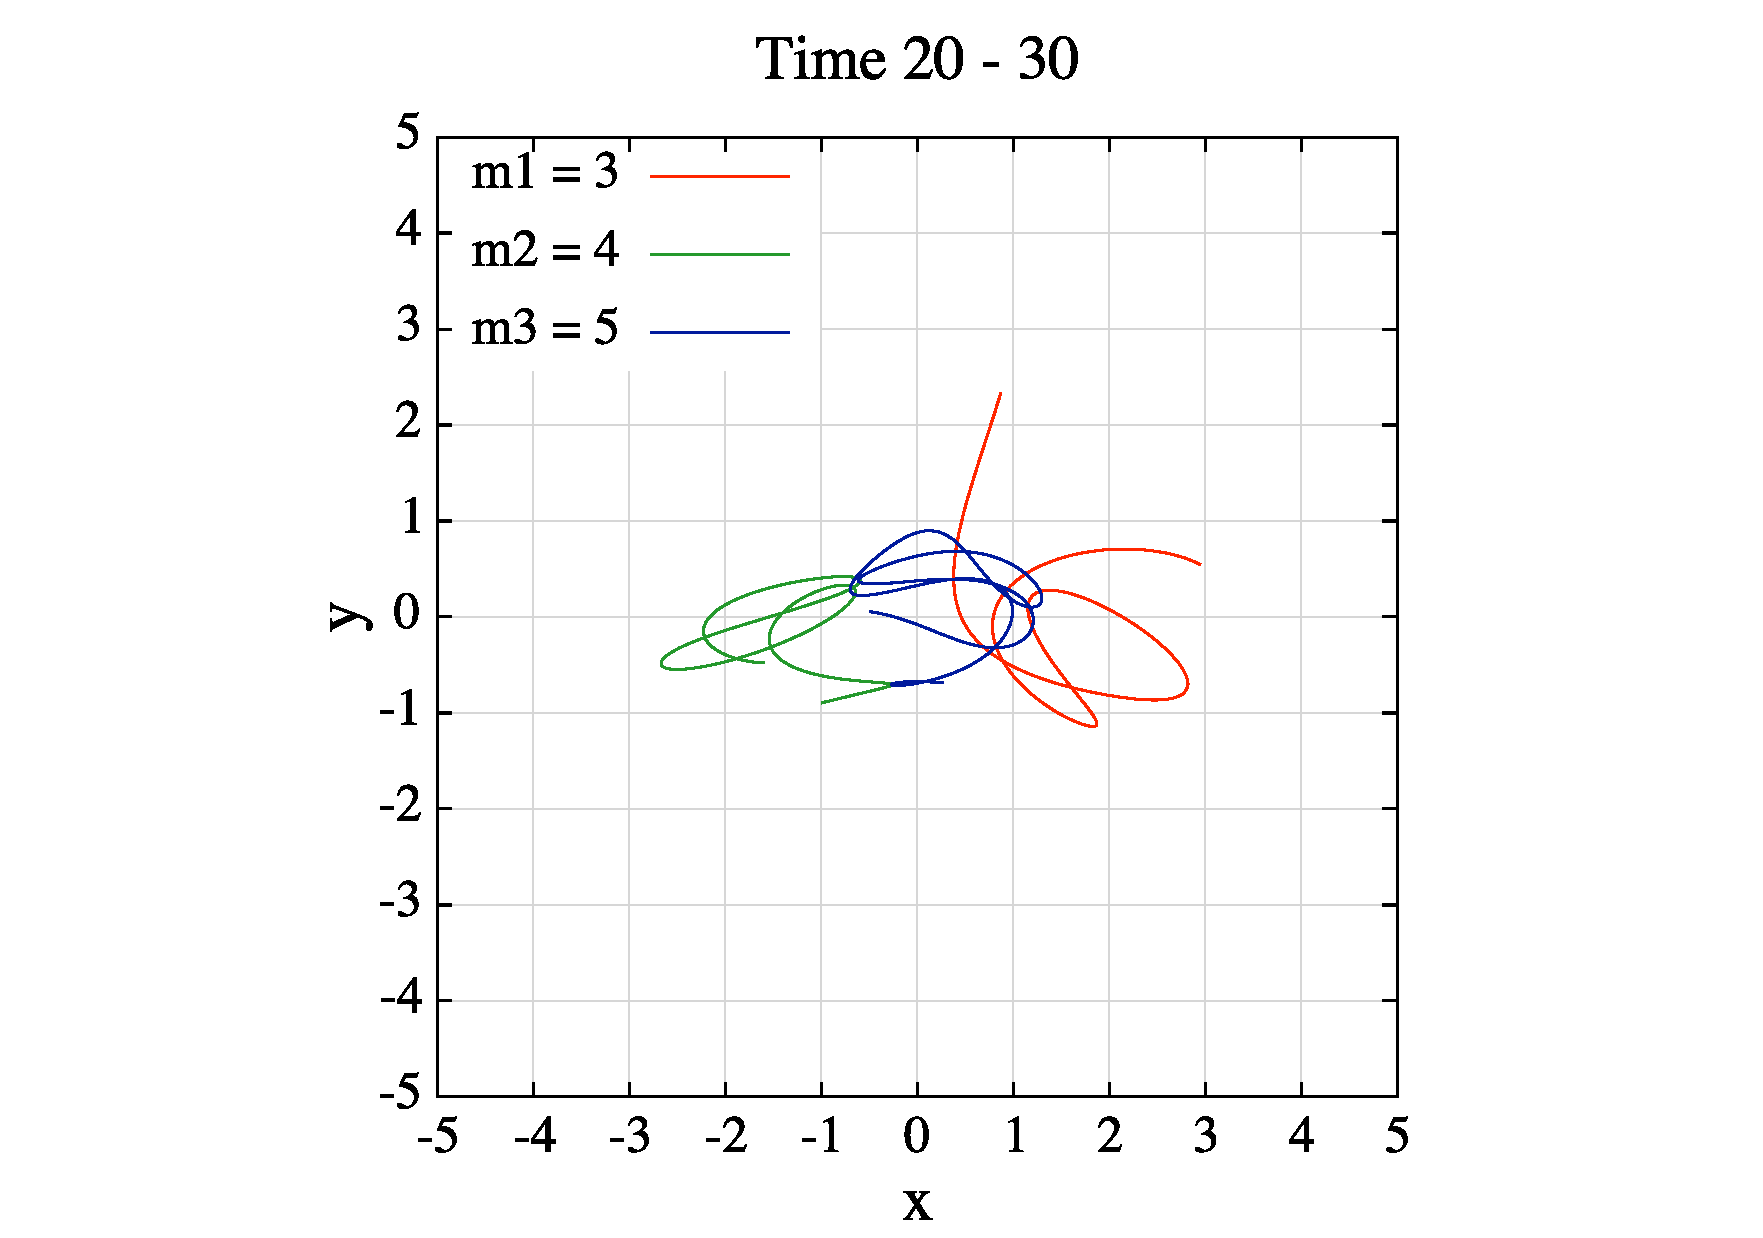
\includegraphics[width=8cm]{./image/pythagoras_orbit_20to30.pdf}
\end{minipage} &
%右
\begin{minipage}[t]{0.45\hsize}
\centering
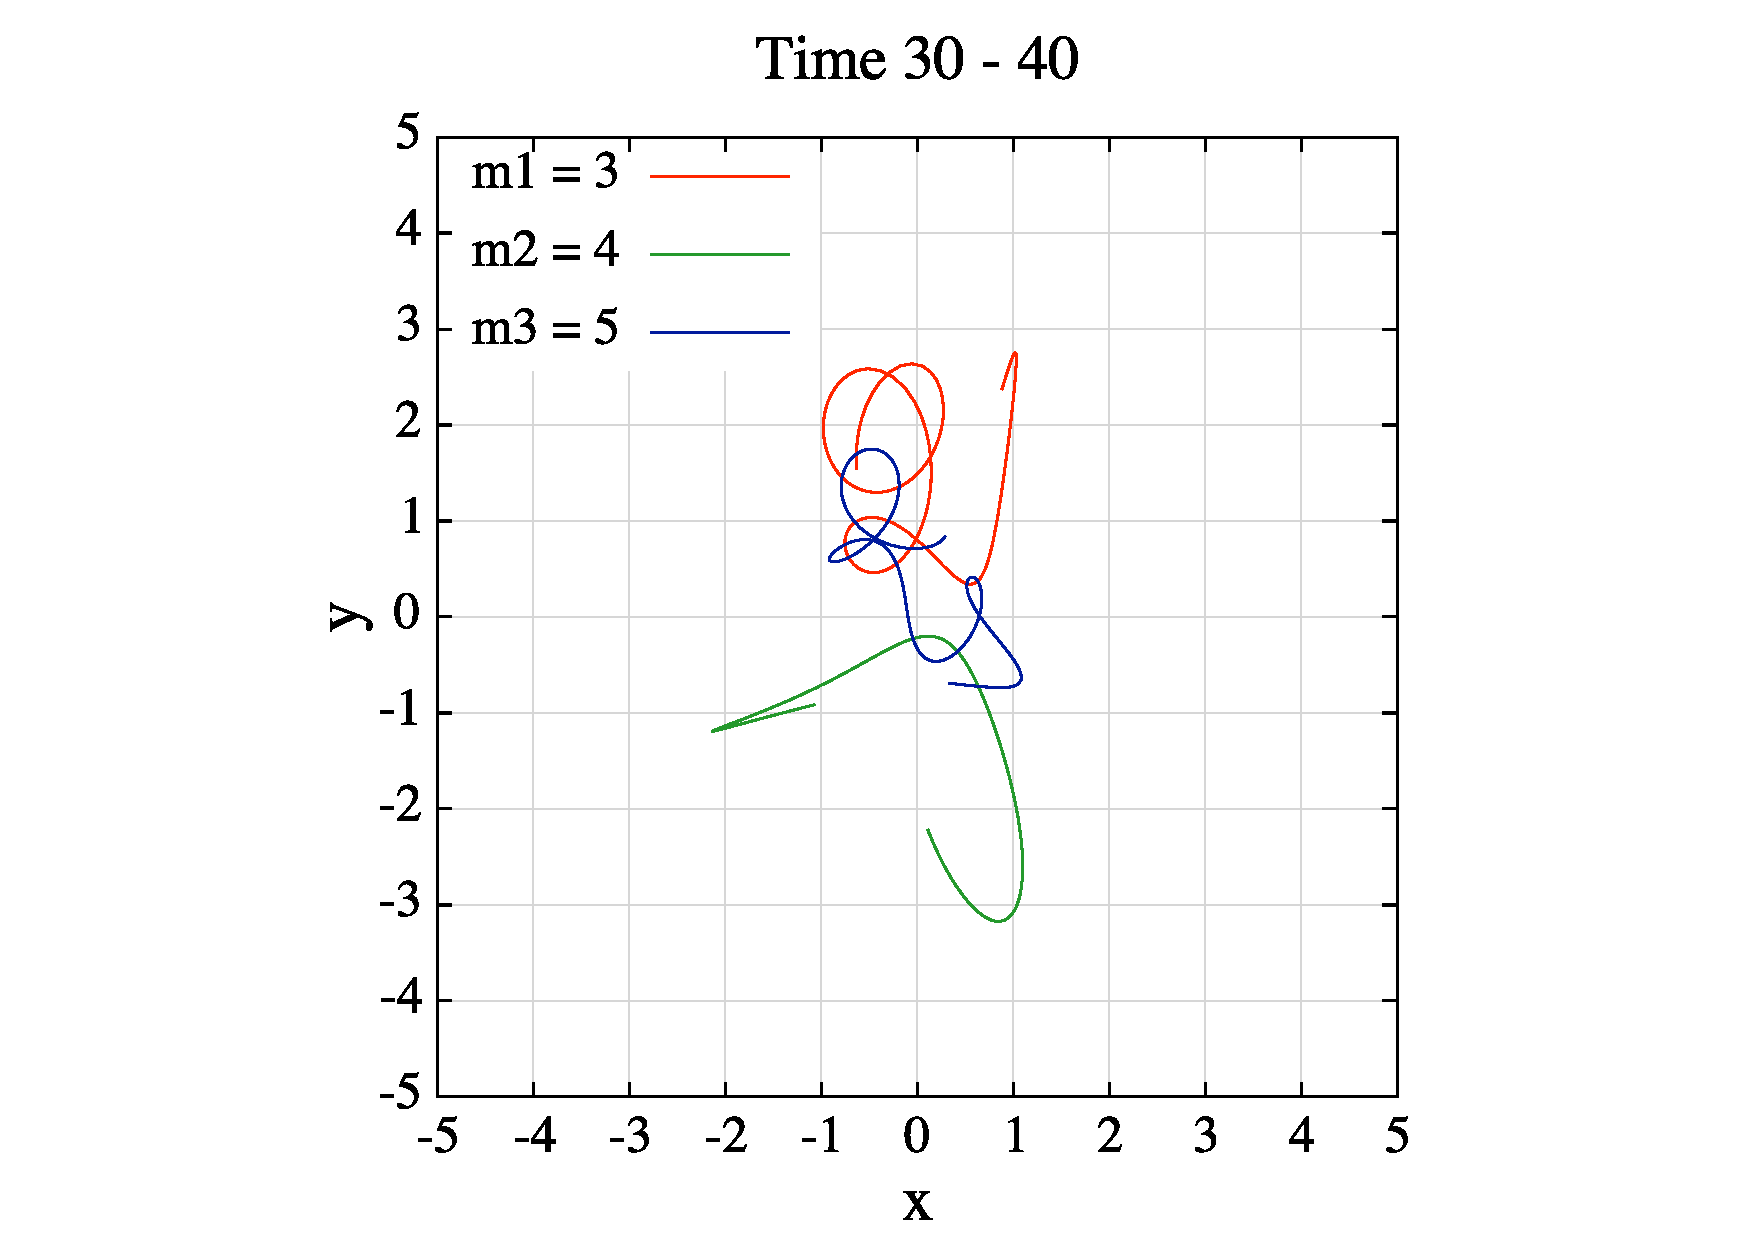
\includegraphics[width=8cm]{./image/pythagoras_orbit_30to40.pdf}
\end{minipage}\\
%
%左
\begin{minipage}[t]{0.45\hsize}
\centering
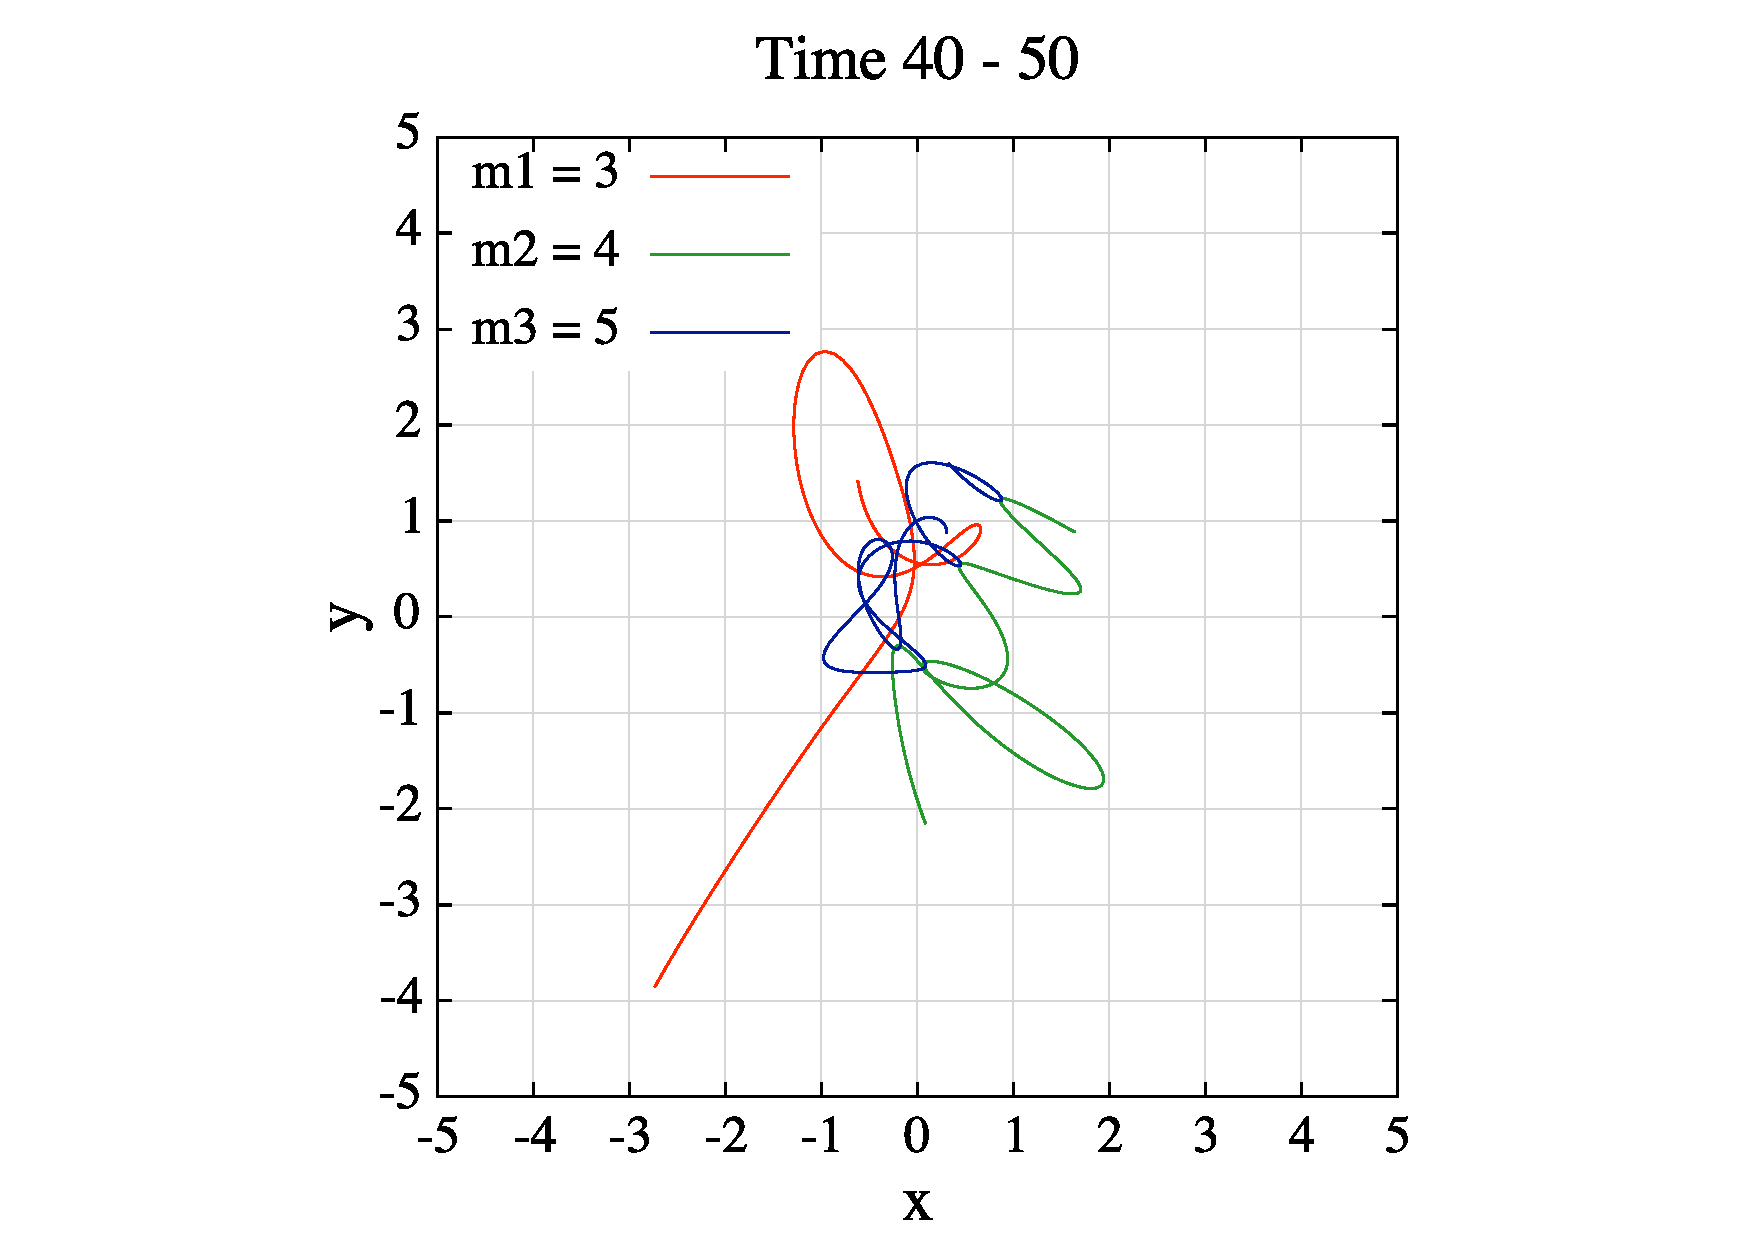
\includegraphics[width=8cm]{./image/pythagoras_orbit_40to50.pdf}
\end{minipage} &
%右
\begin{minipage}[t]{0.45\hsize}
\centering
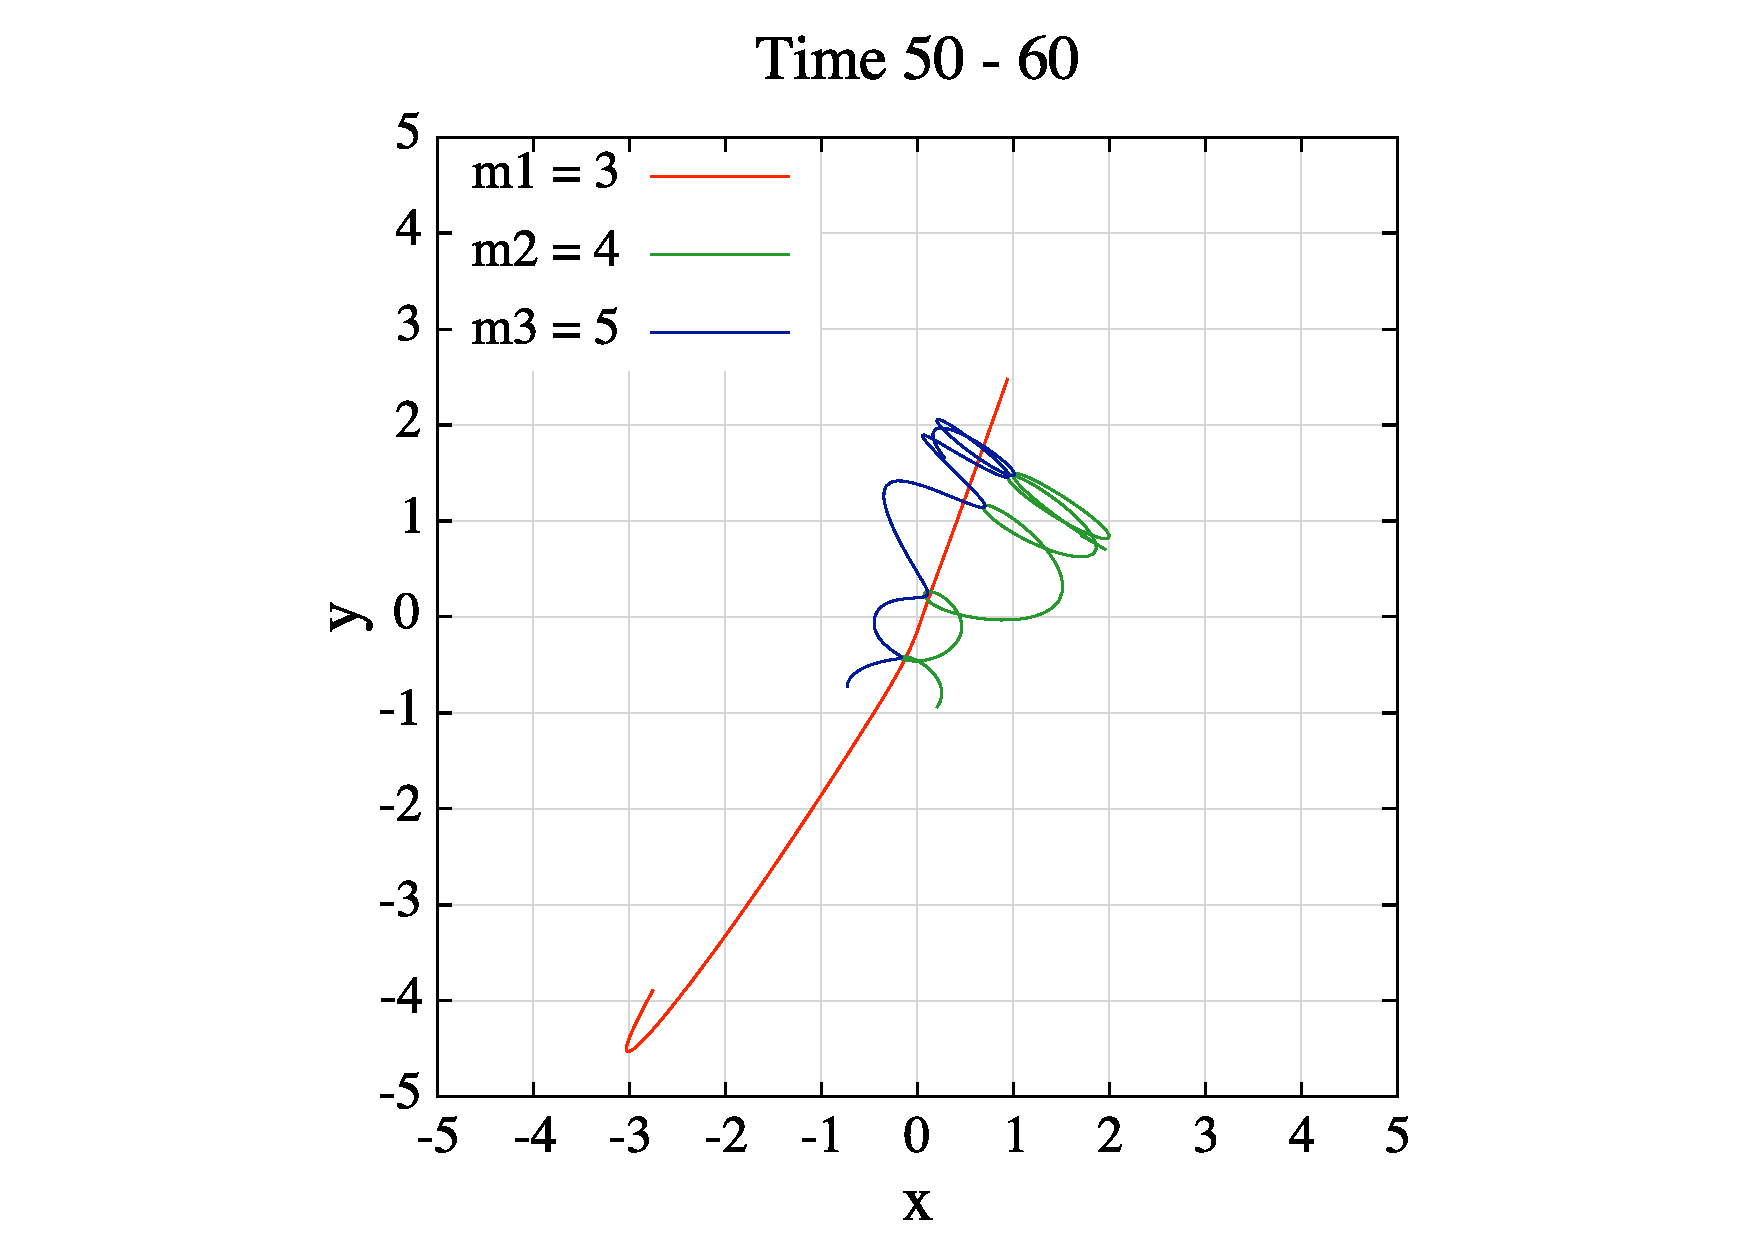
\includegraphics[width=8cm]{./image/pythagoras_orbit_50to60.pdf}
\end{minipage}\\
%
\begin{minipage}[t]{0.45\hsize}
\centering
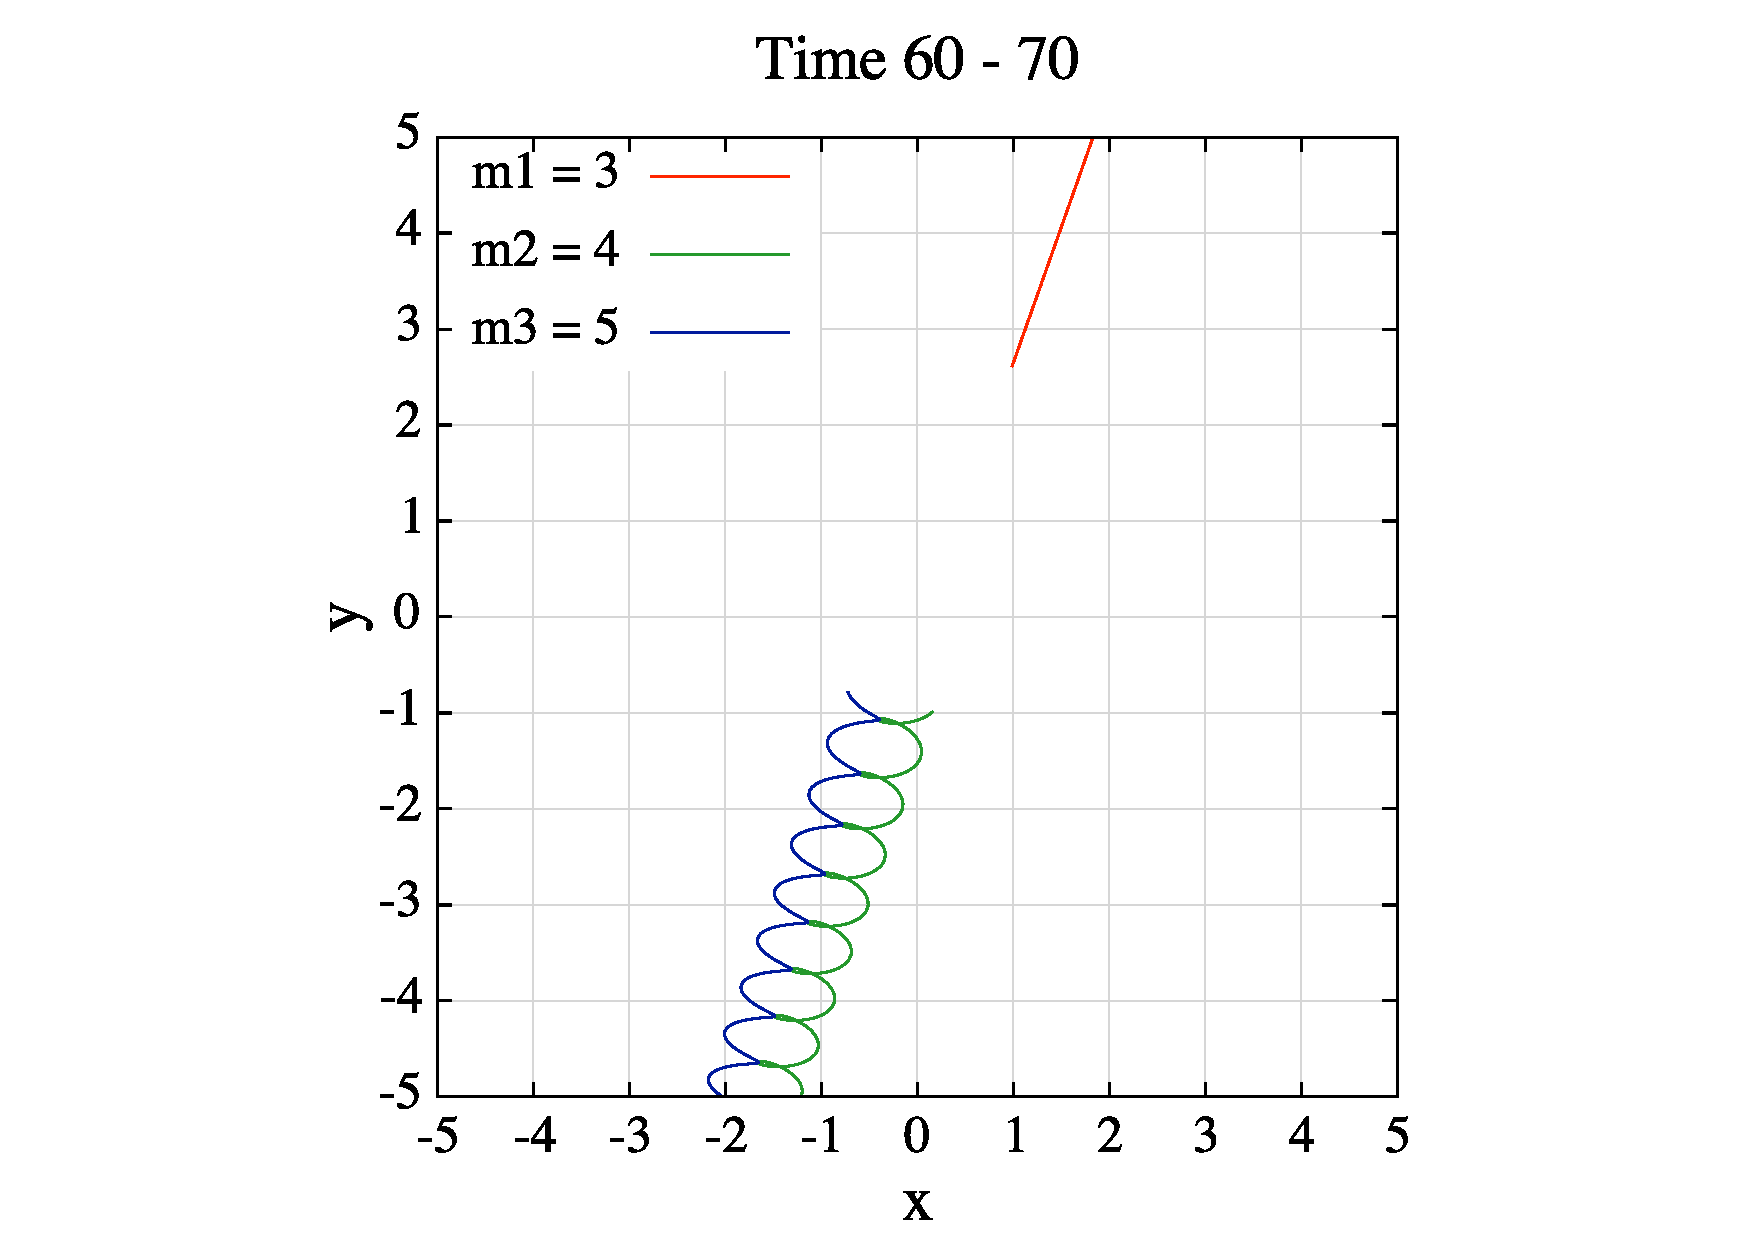
\includegraphics[width=8cm]{./image/pythagoras_orbit_60to70.pdf}
\end{minipage}
\end{tabular}
\caption{\label{}}
\end{figure}


\begin{figure}[H]
\centering
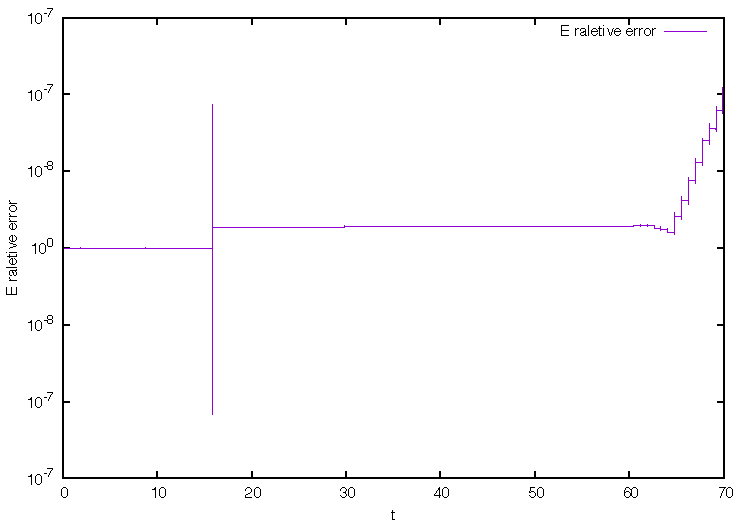
\includegraphics[width=10cm]{./image/pythagoras_E_error.pdf}
\caption{\label{}}
\end{figure}

\begin{figure}[H]
\centering
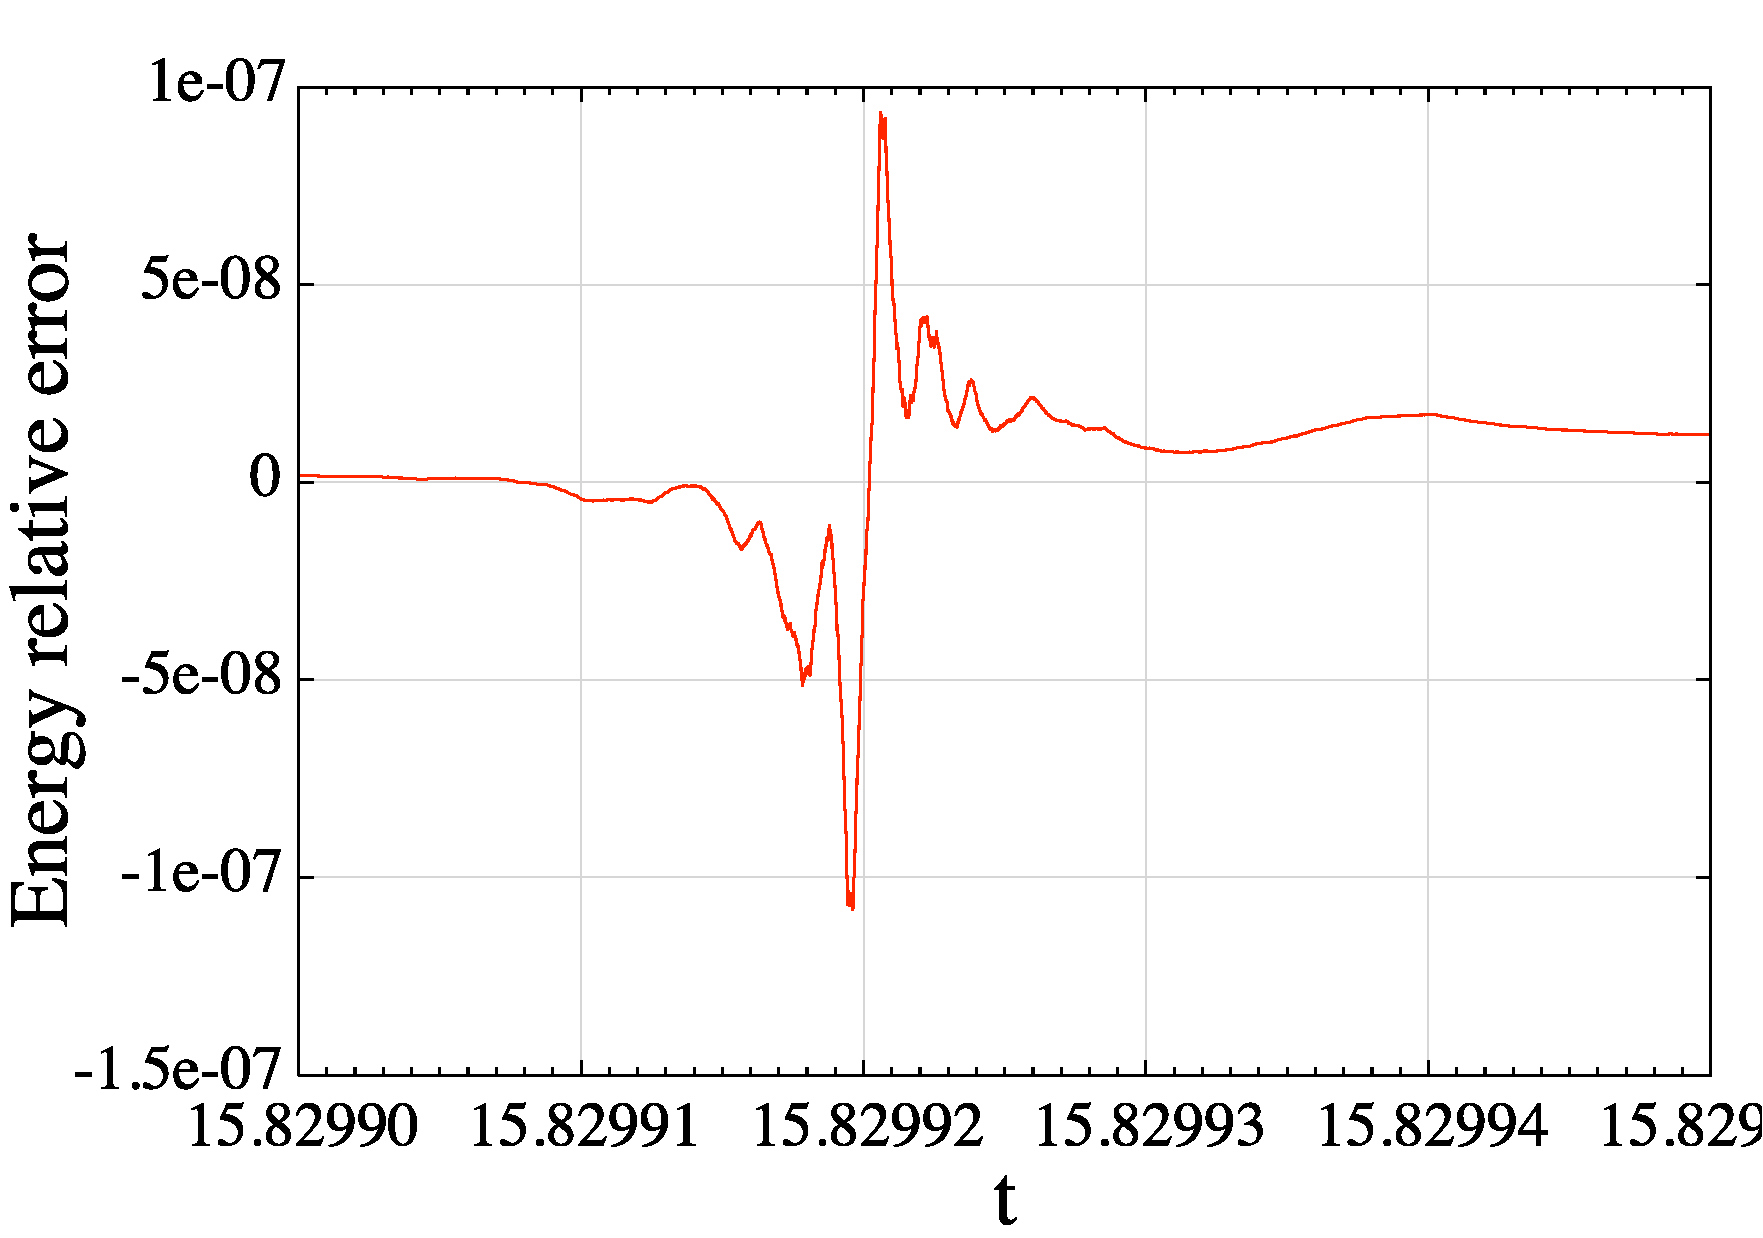
\includegraphics[width=10cm]{./image/pythagoras_E_error_detail.pdf}
\caption{\label{}}
\end{figure}

\section{本計算}
\subsection{Kuiper Belt}



\subsection{Asteroid Belt}



\subsection{Secular Resonance}

\subsubsection{現在から100万年後までの巨大惑星の運動}


\begin{figure}[H]
\begin{tabular}{cc}
%左
\begin{minipage}[t]{0.45\hsize}
\centering
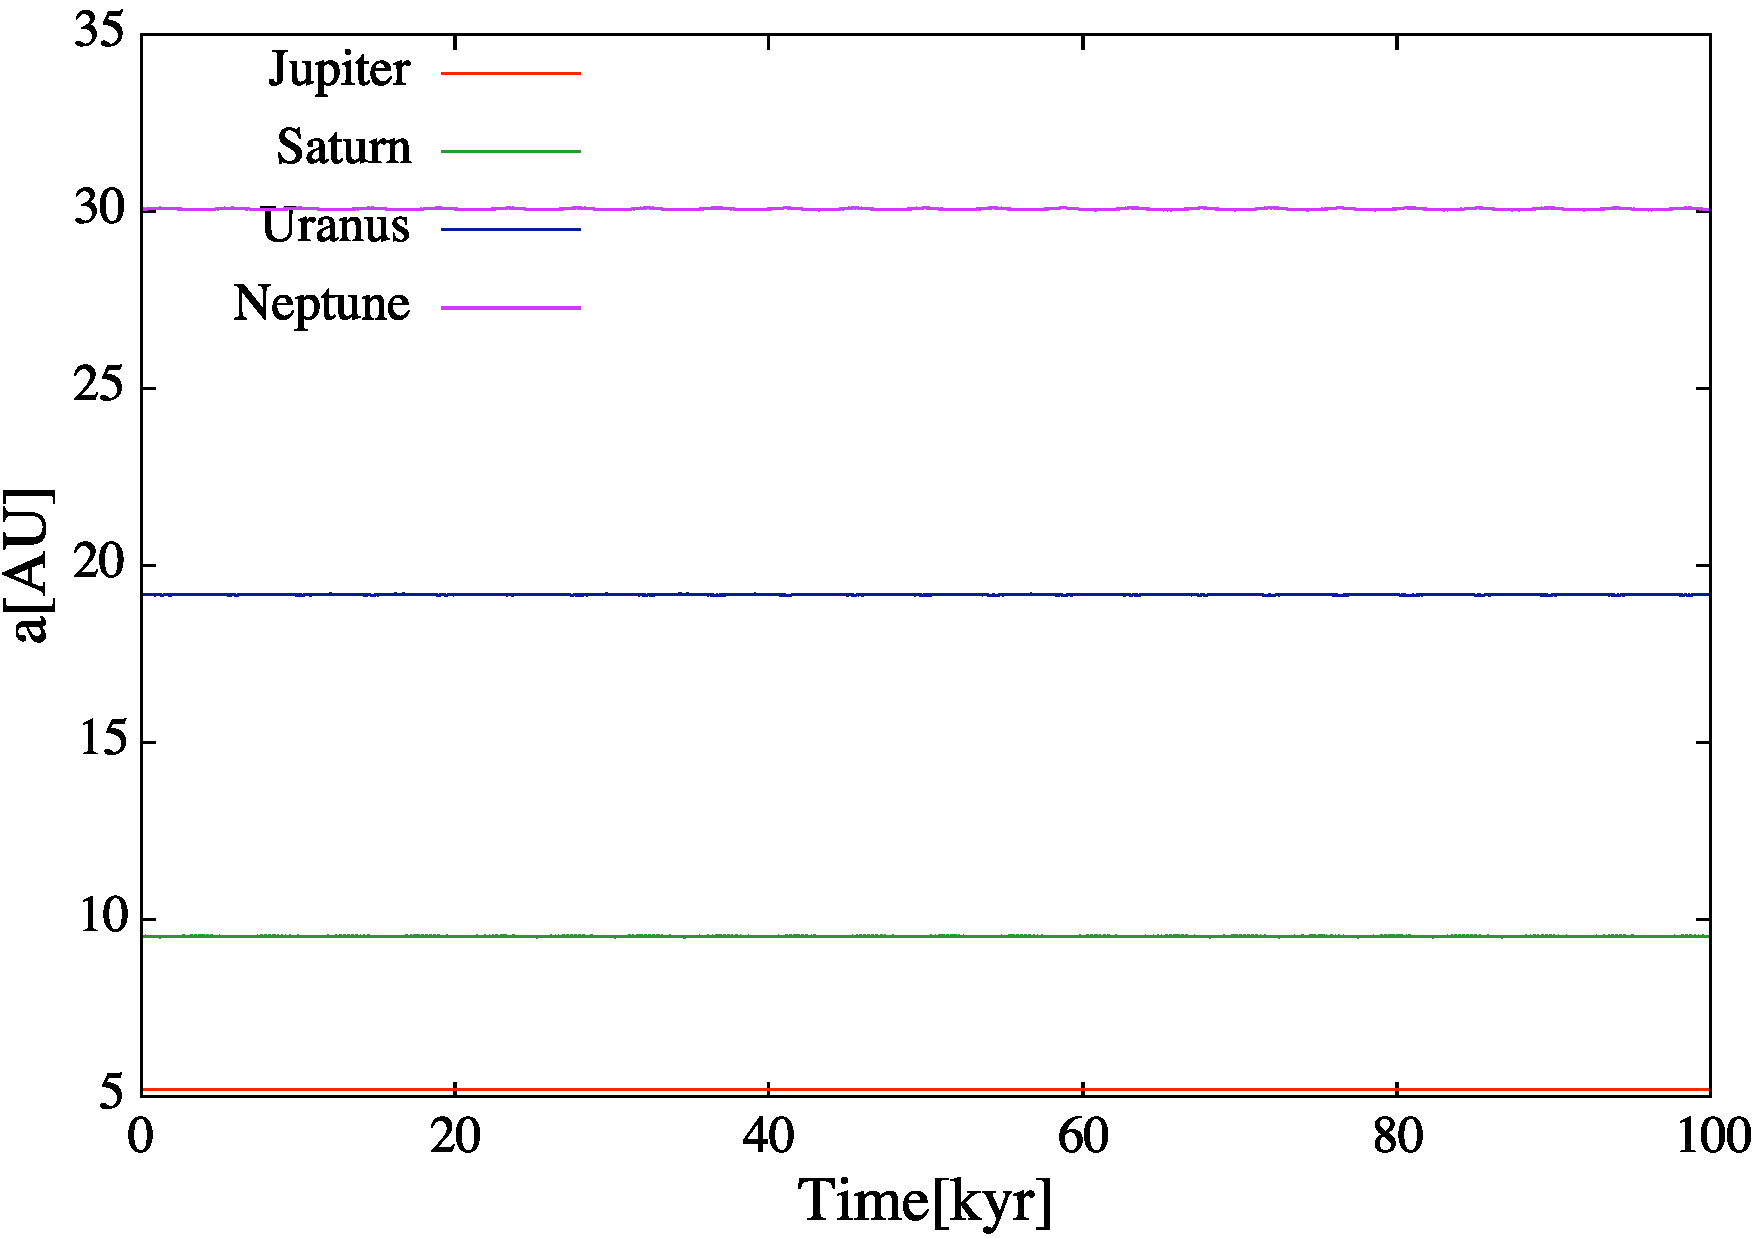
\includegraphics[width=7.6cm]{./image/Nomove_a_100kyr.pdf}
\end{minipage} &
%右
\begin{minipage}[t]{0.45\hsize}
\centering
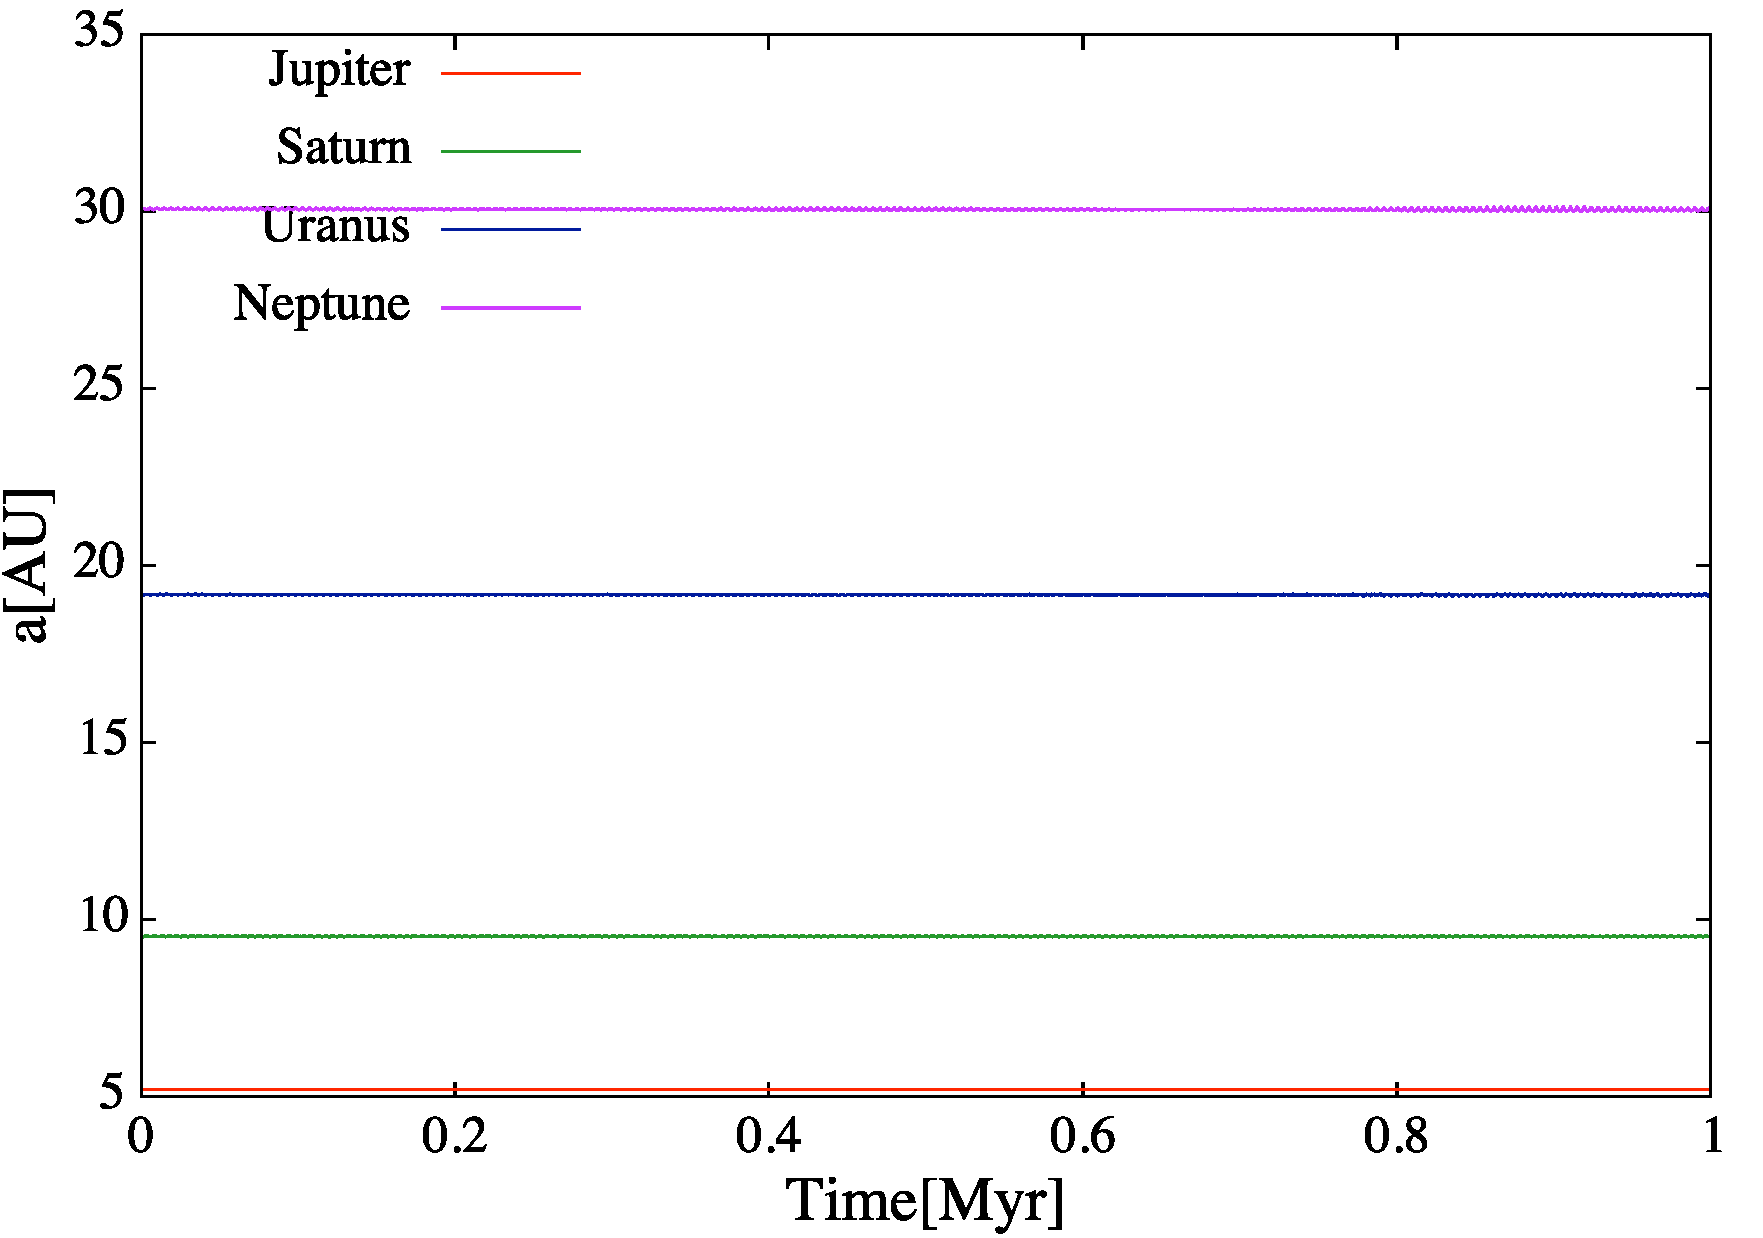
\includegraphics[width=7.6cm]{./image/Nomove_a_1Myr.pdf}
\end{minipage}
%
\end{tabular}
\caption{\label{}}
\end{figure}


\begin{figure}[H]
\begin{tabular}{cc}
%左
\begin{minipage}[t]{0.45\hsize}
\centering
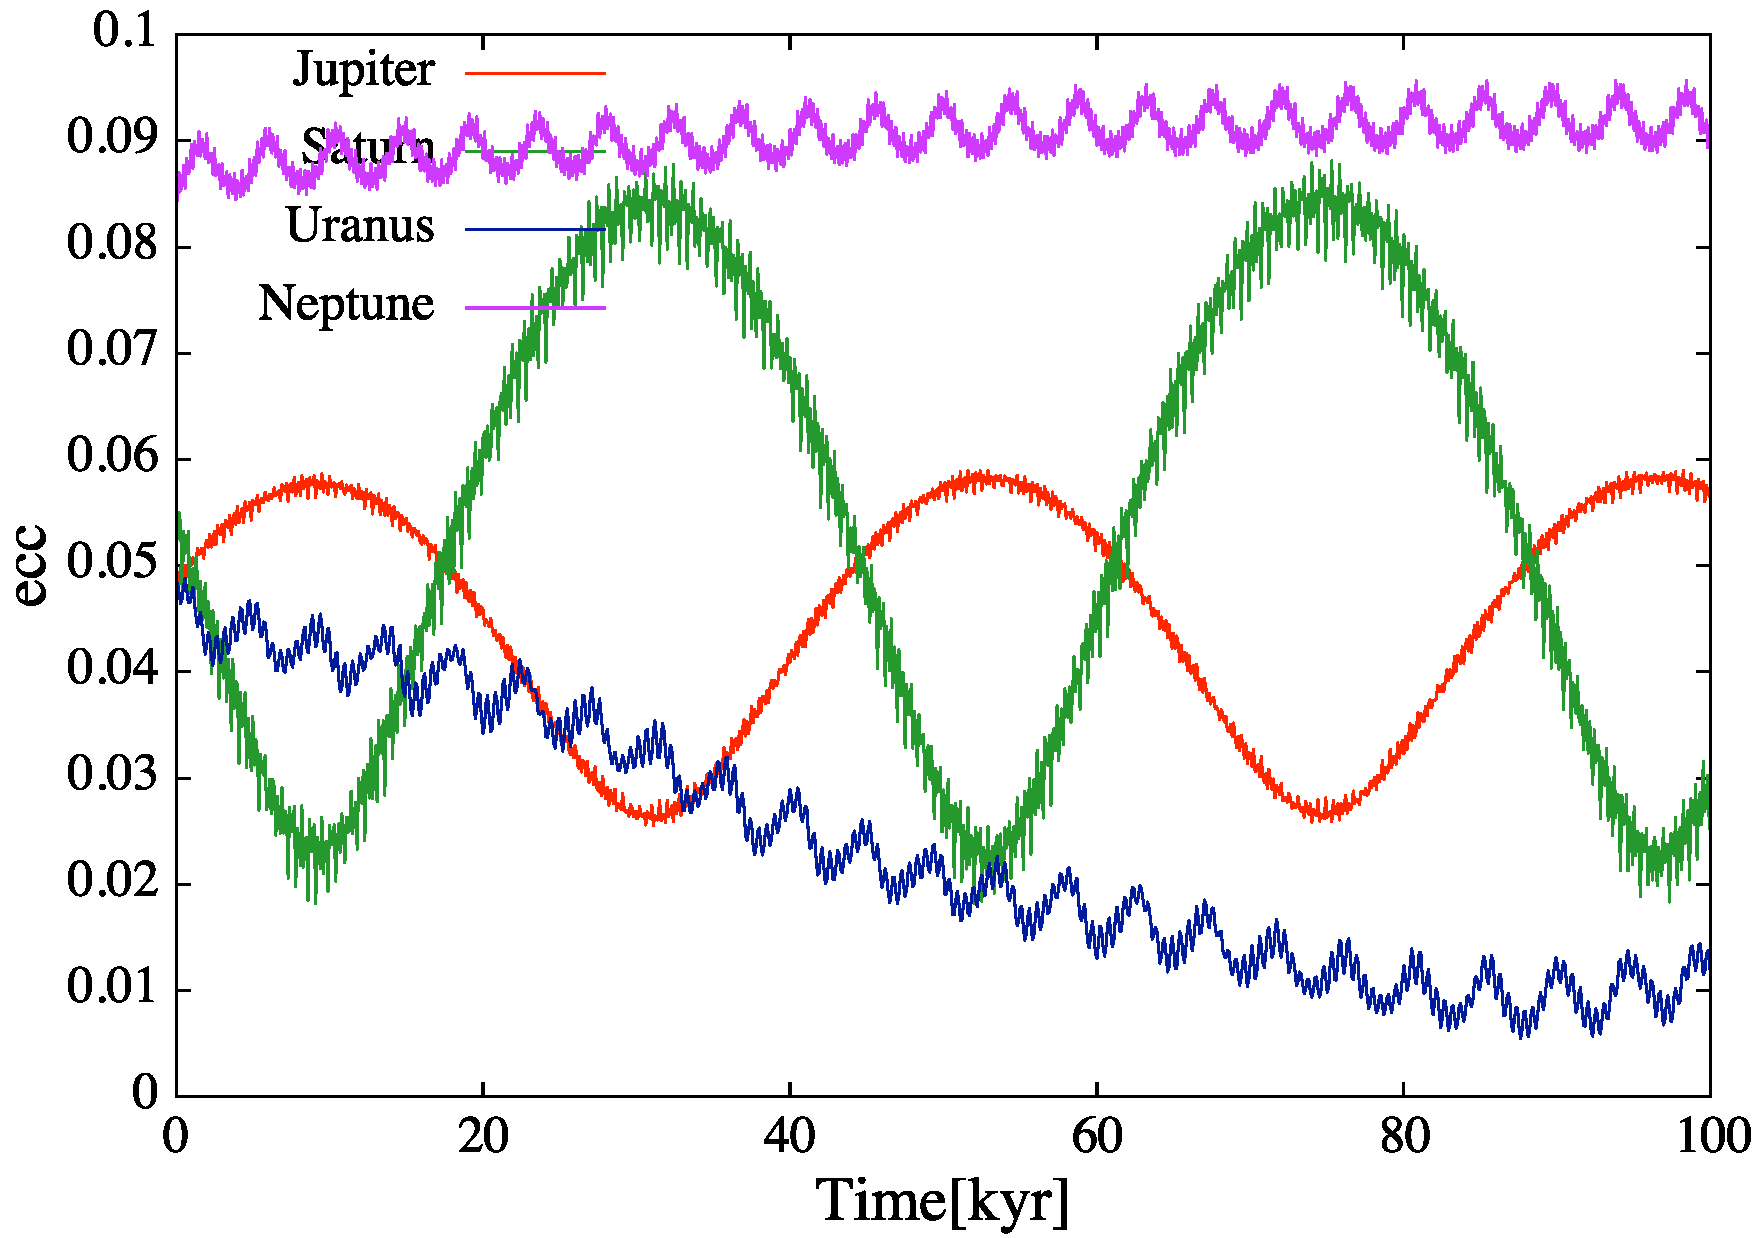
\includegraphics[width=7.6cm]{./image/Nomove_ecc_100kyr.pdf}
\end{minipage} &
%右
\begin{minipage}[t]{0.45\hsize}
\centering
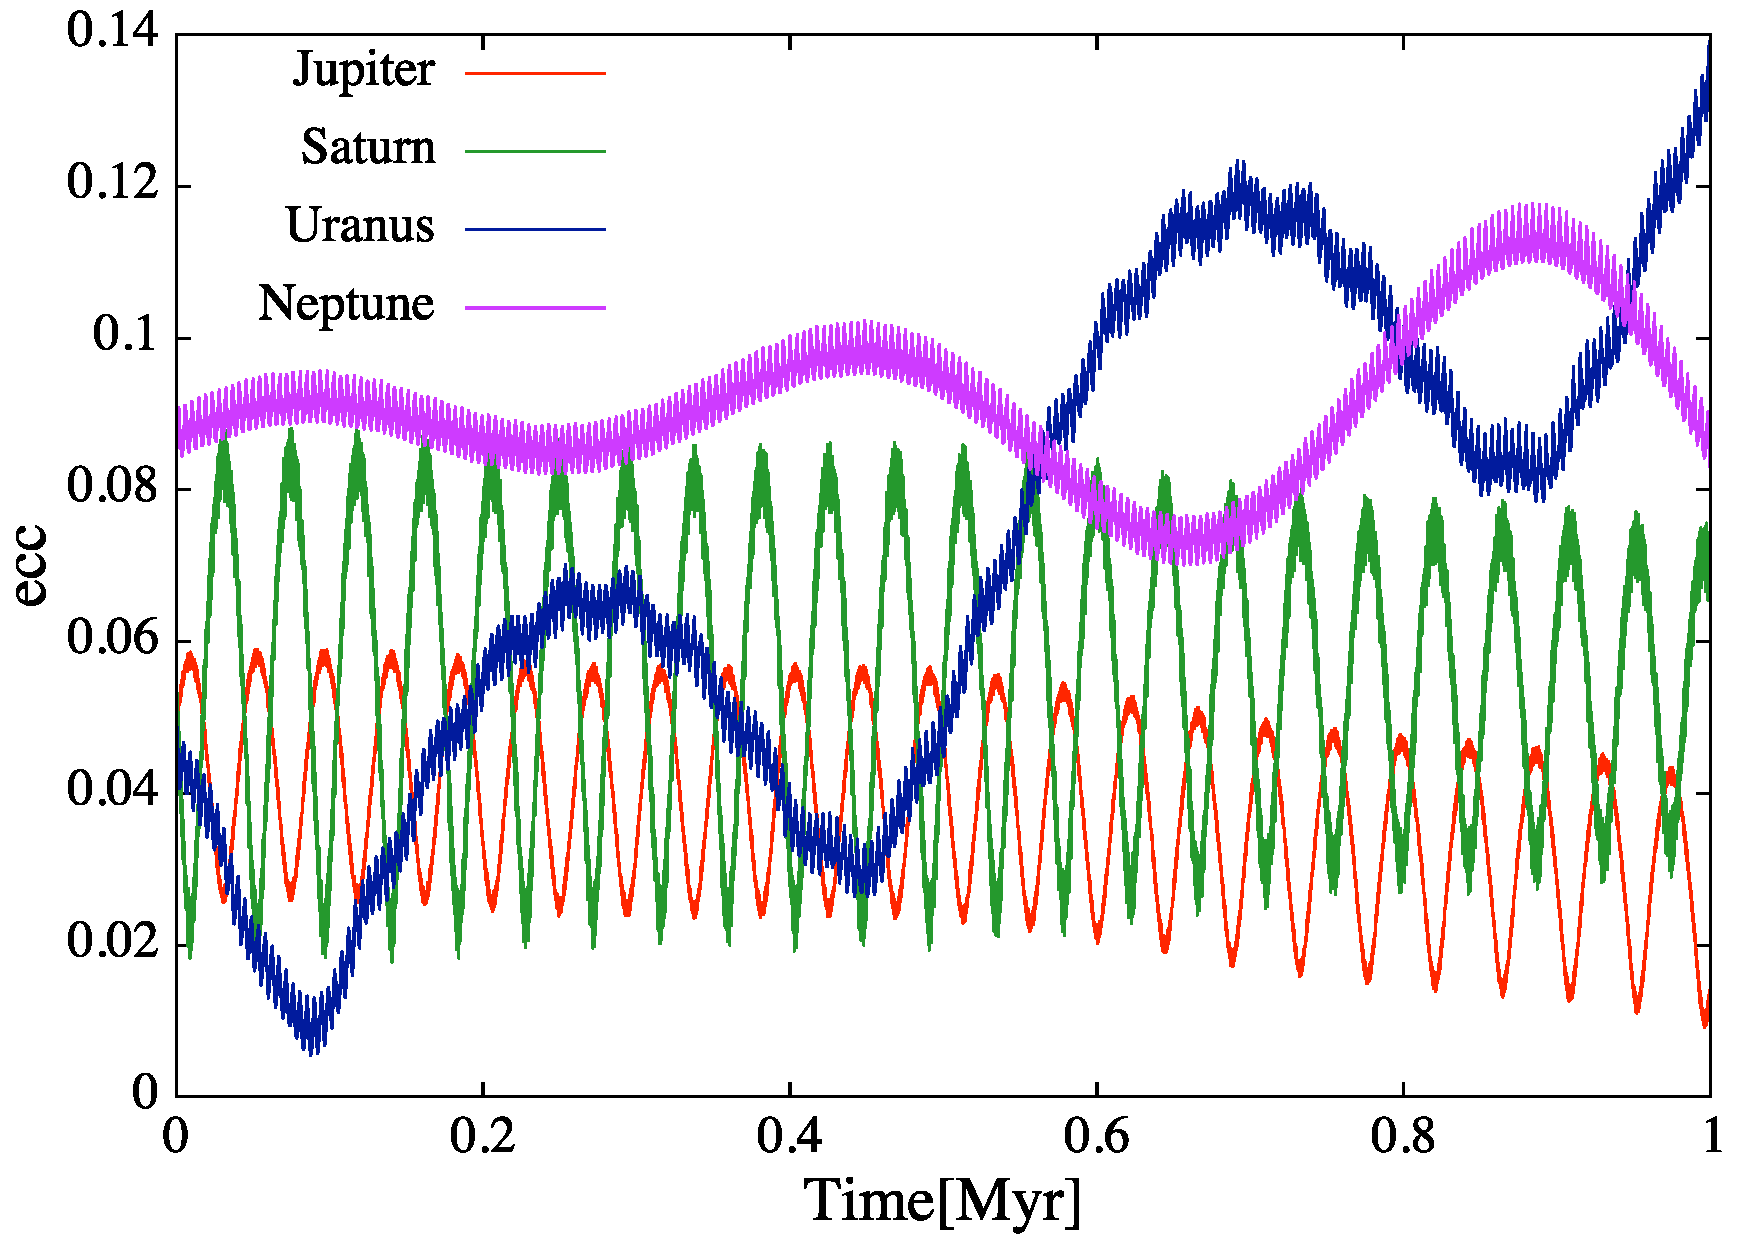
\includegraphics[width=7.6cm]{./image/Nomove_ecc_1Myr.pdf}
\end{minipage}
%
\end{tabular}
\caption{\label{}}
\end{figure}


\begin{figure}[H]
\begin{tabular}{cc}
%左
\begin{minipage}[t]{0.45\hsize}
\centering
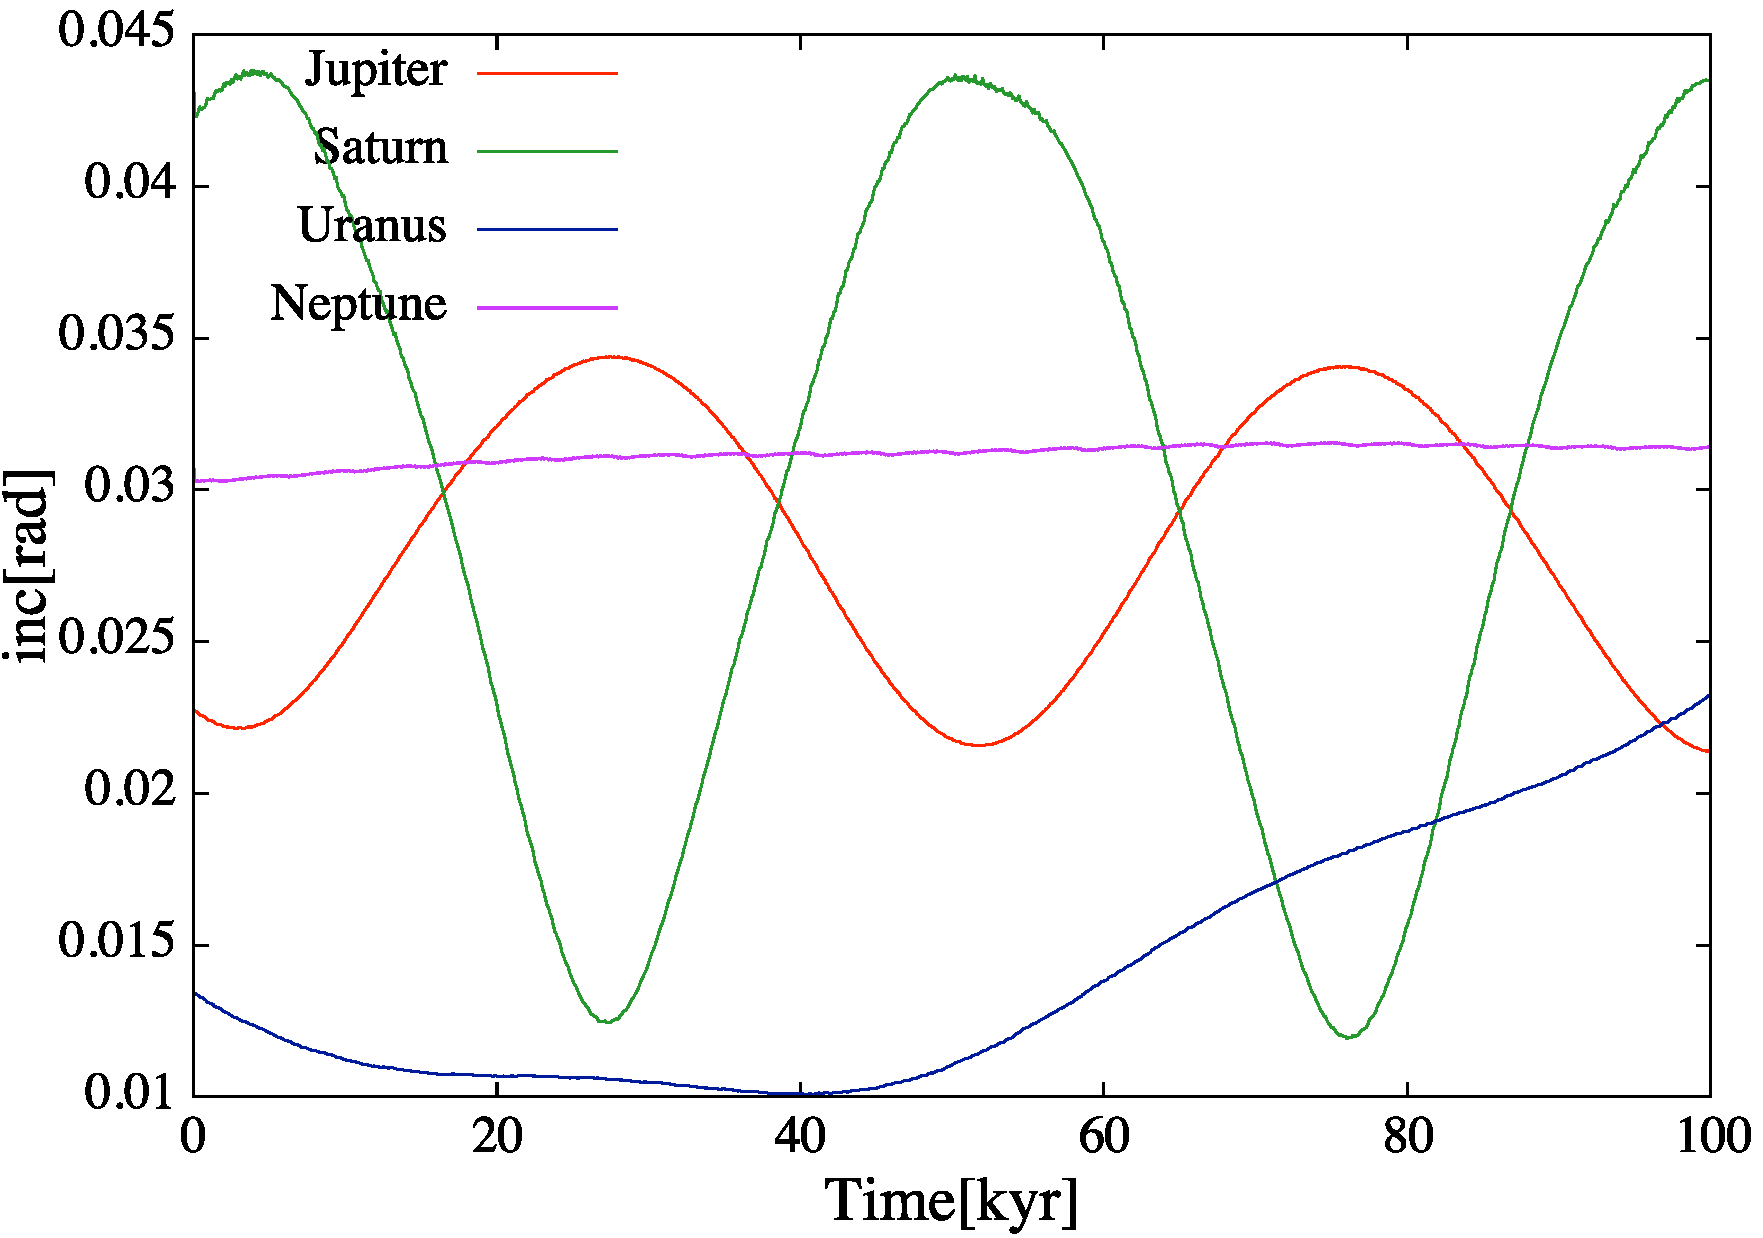
\includegraphics[width=7.6cm]{./image/Nomove_inc_100kyr.pdf}
\end{minipage} &
%右
\begin{minipage}[t]{0.45\hsize}
\centering
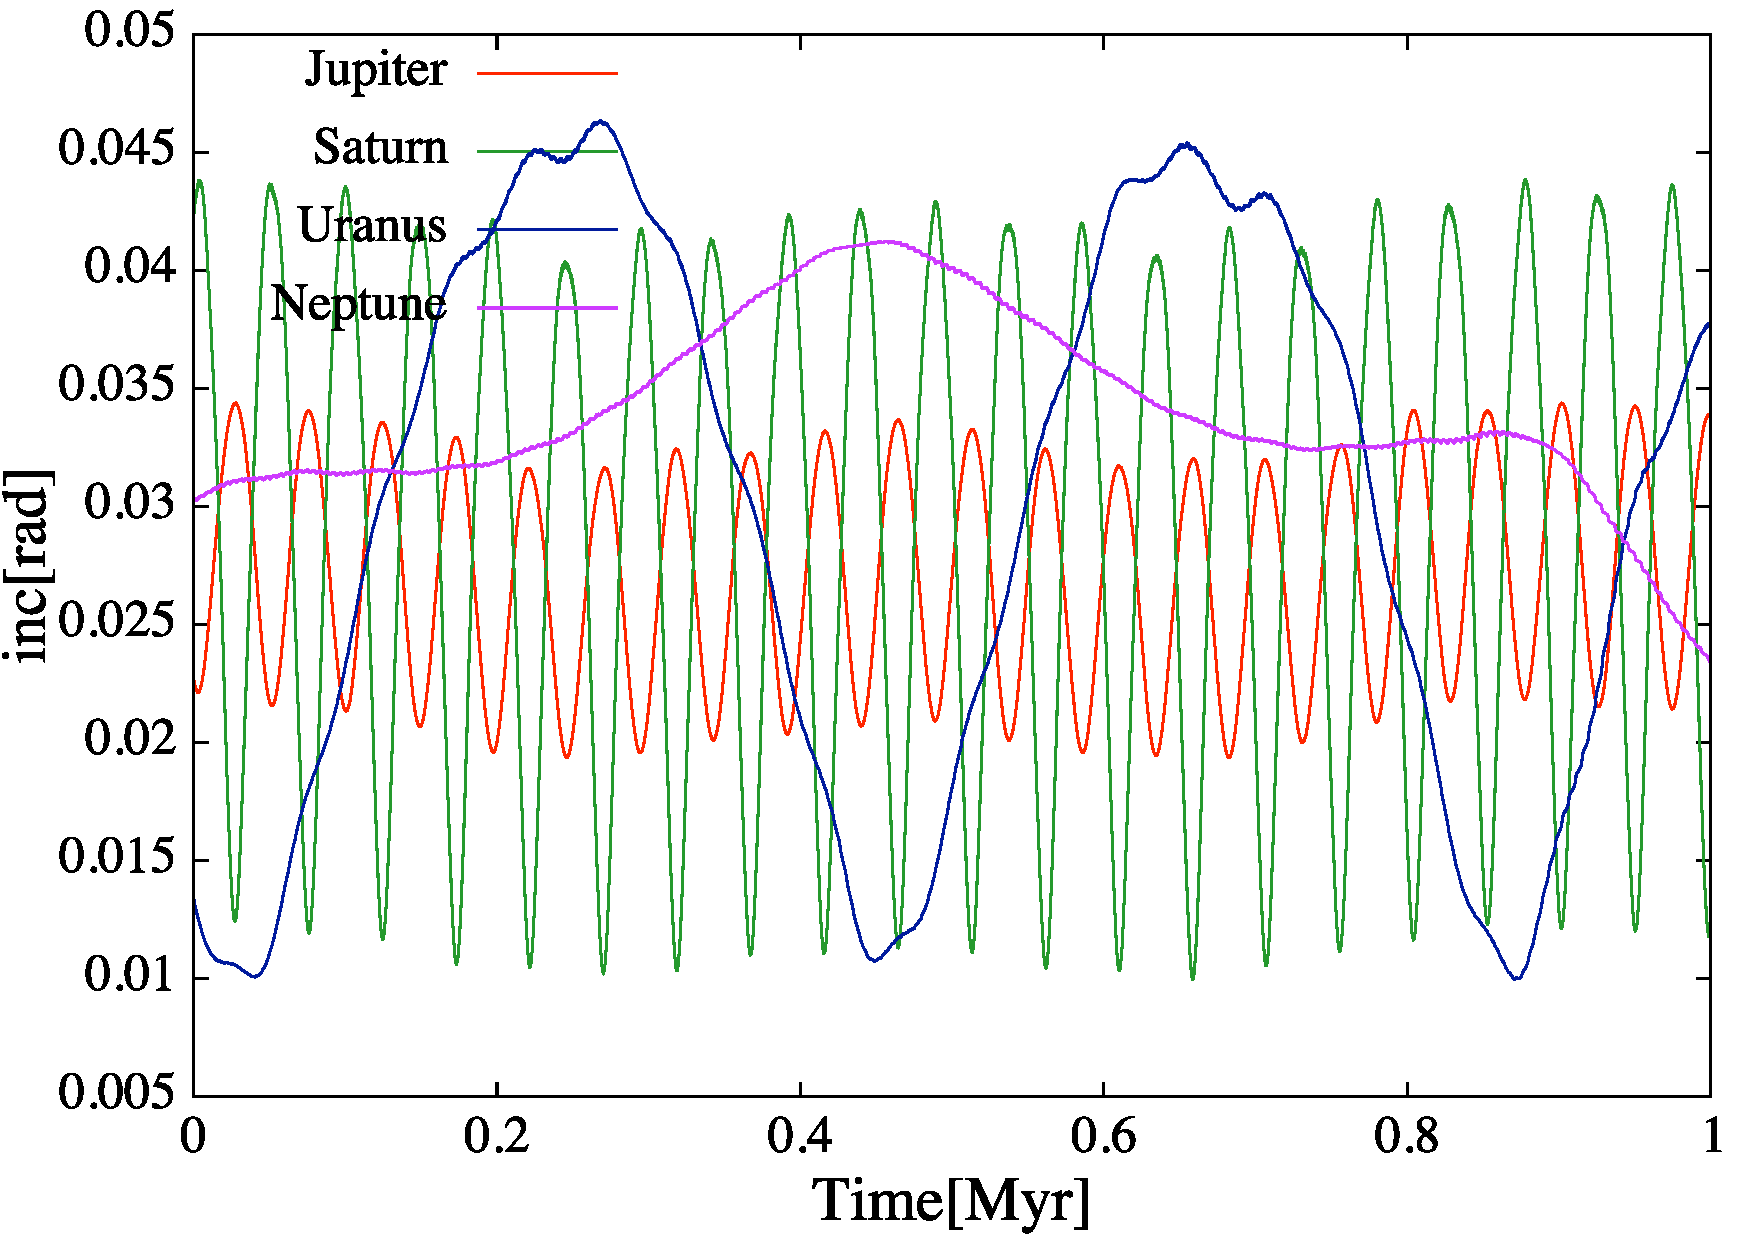
\includegraphics[width=7.6cm]{./image/Nomove_inc_1Myr.pdf}
\end{minipage}
%
\end{tabular}
\caption{\label{}}
\end{figure}


\begin{figure}[H]
\begin{tabular}{cc}
%左
\begin{minipage}[t]{0.45\hsize}
\centering
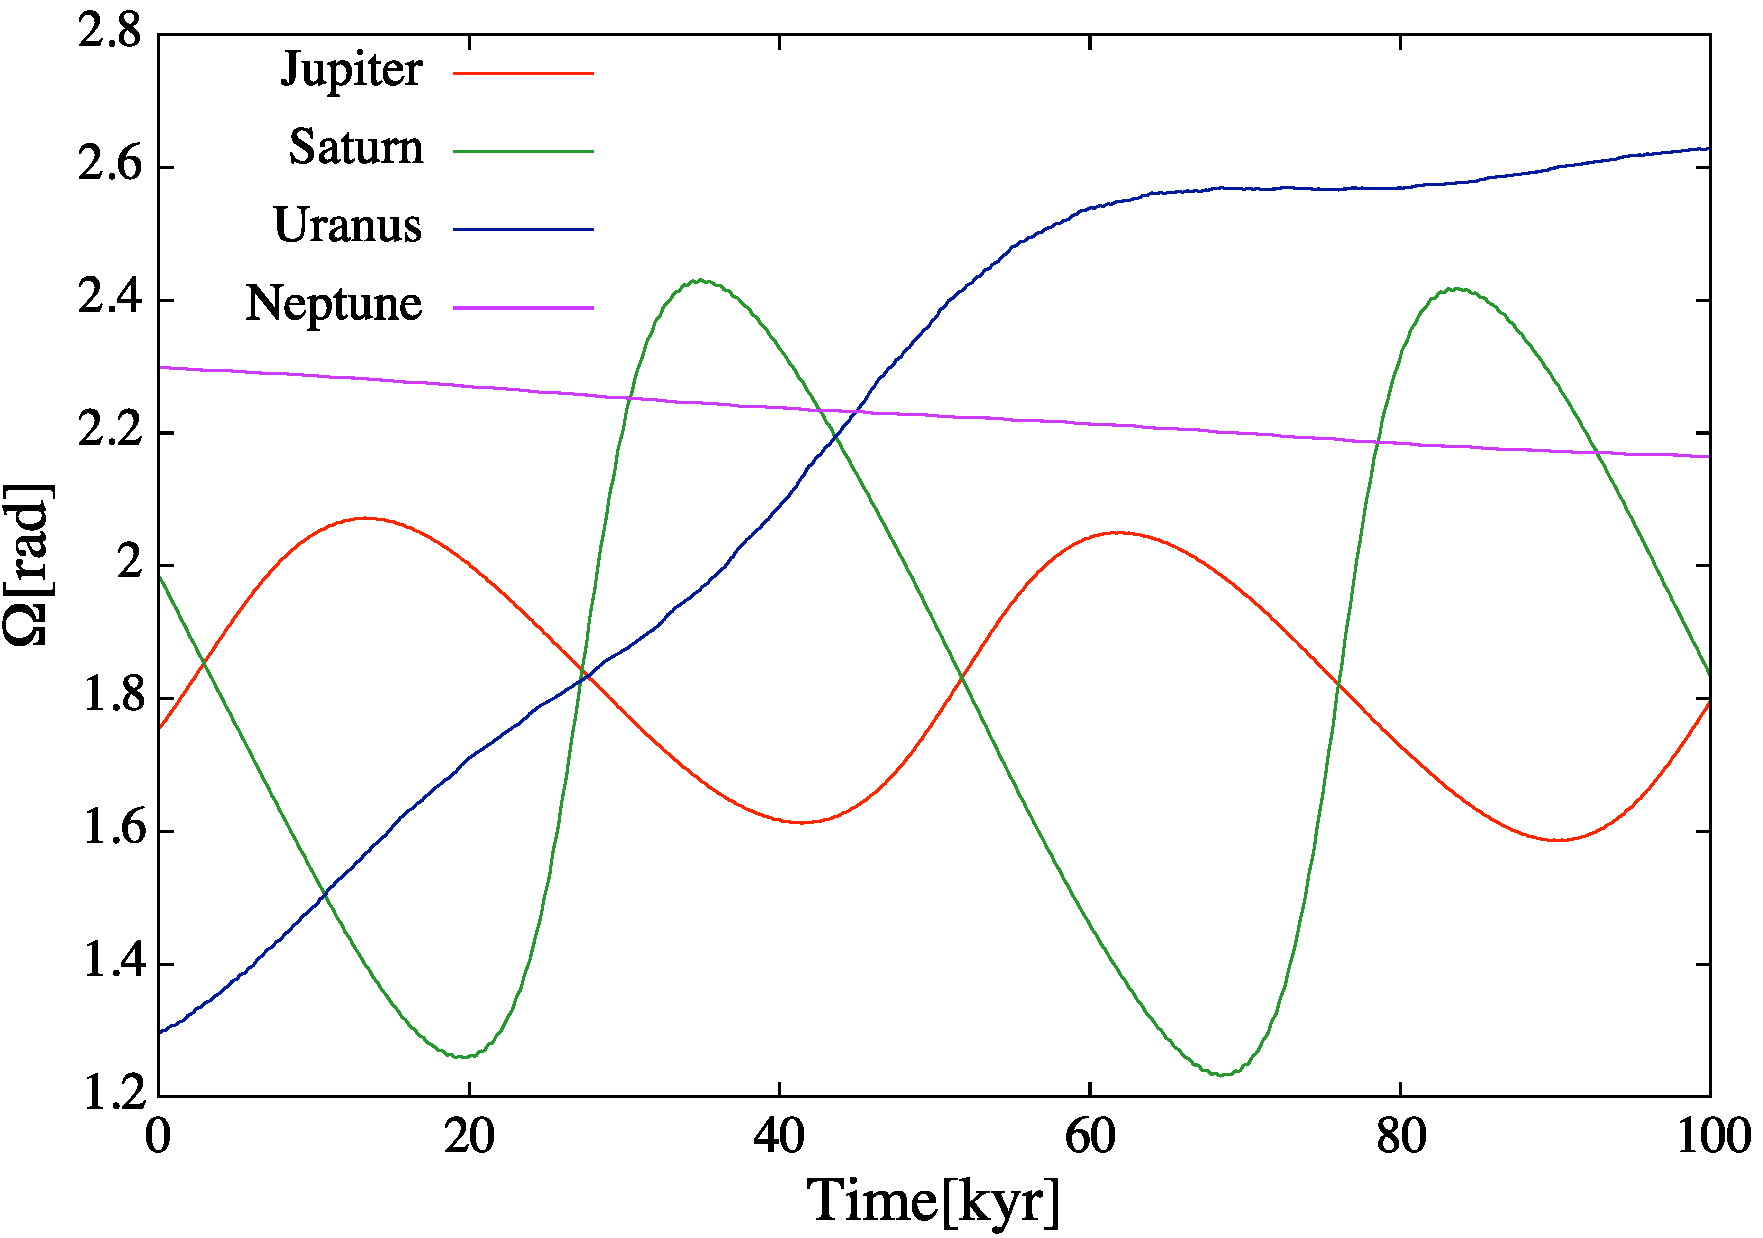
\includegraphics[width=7.6cm]{./image/Nomove_capitalOMEGA_100kyr.pdf}
\end{minipage} &
%右
\begin{minipage}[t]{0.45\hsize}
\centering
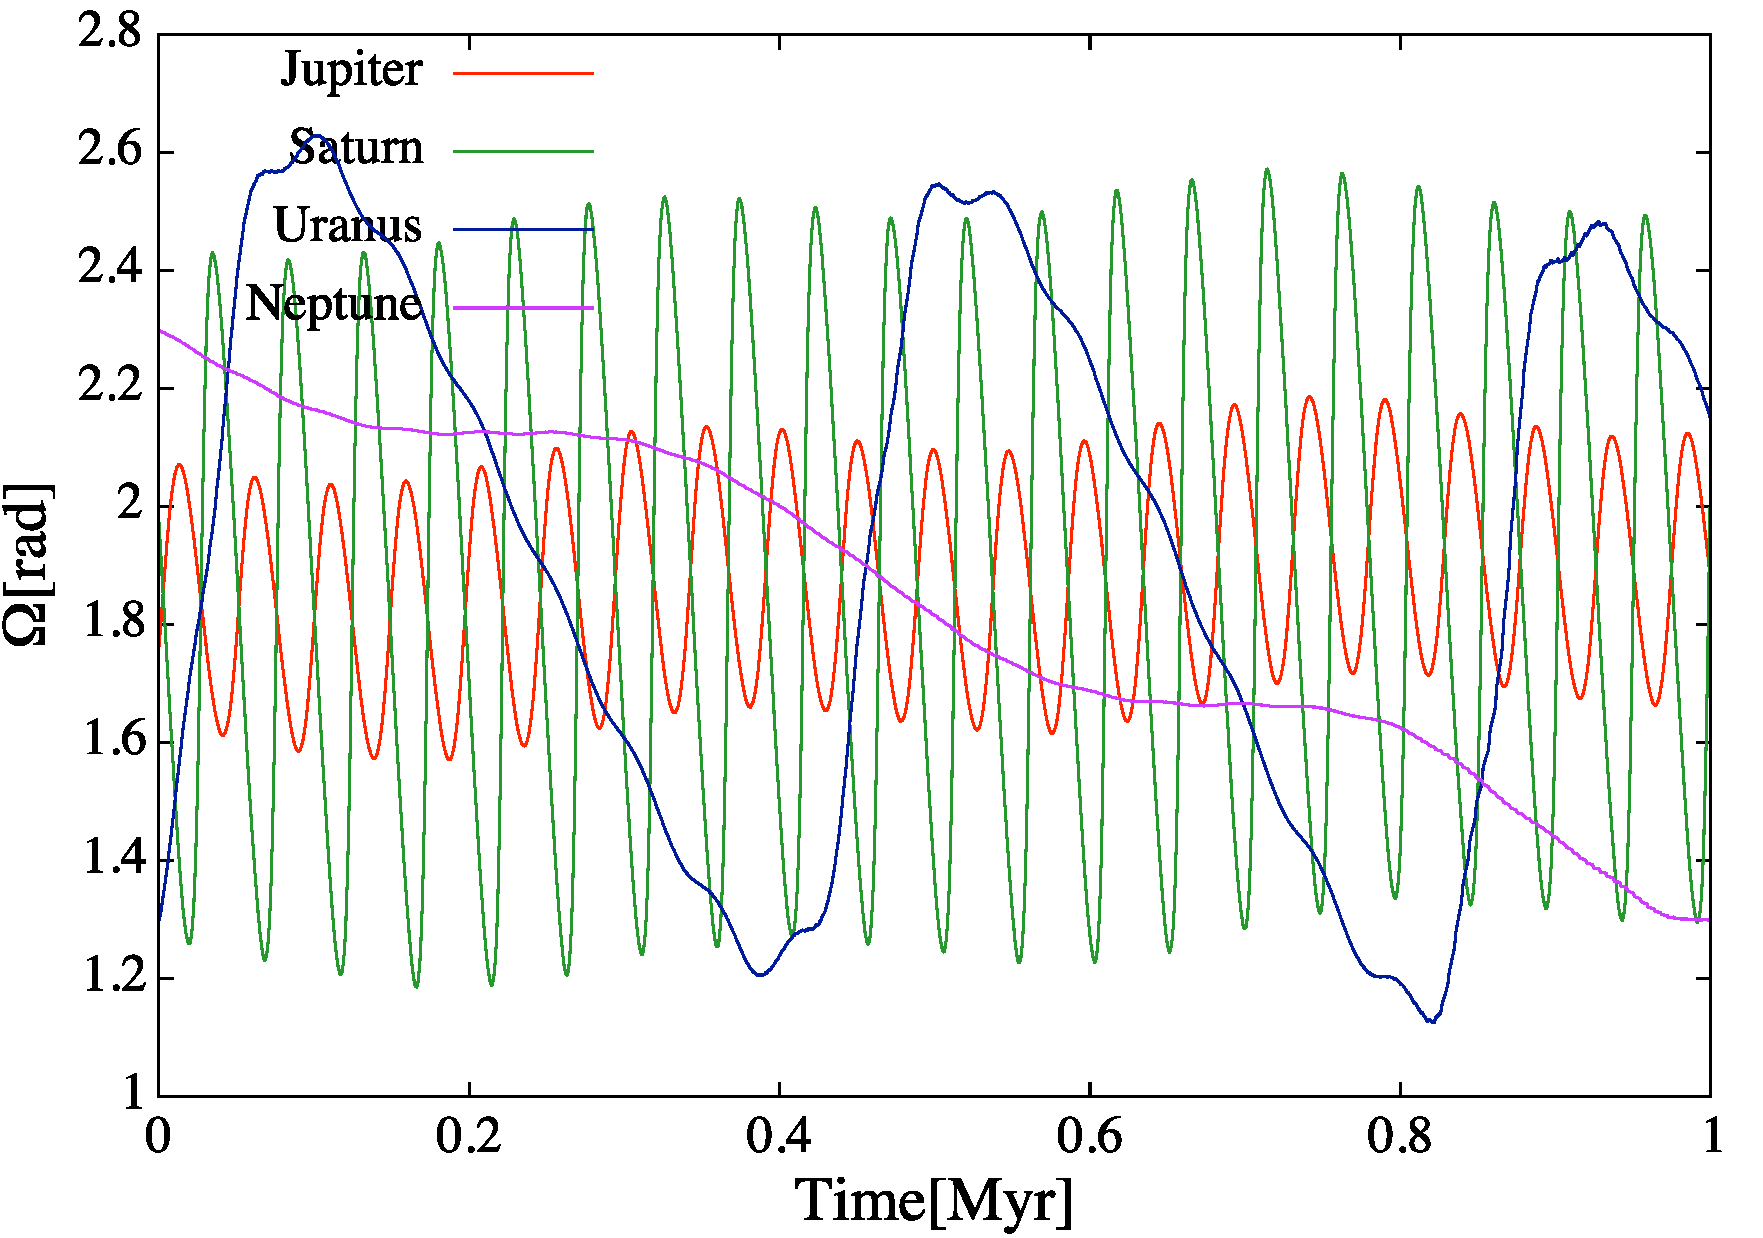
\includegraphics[width=7.6cm]{./image/Nomove_capitalOMEGA_1Myr.pdf}
\end{minipage}
%
\end{tabular}
\caption{\label{}}
\end{figure}


\begin{figure}[H]
\begin{tabular}{cc}
%左
\begin{minipage}[t]{0.45\hsize}
\centering
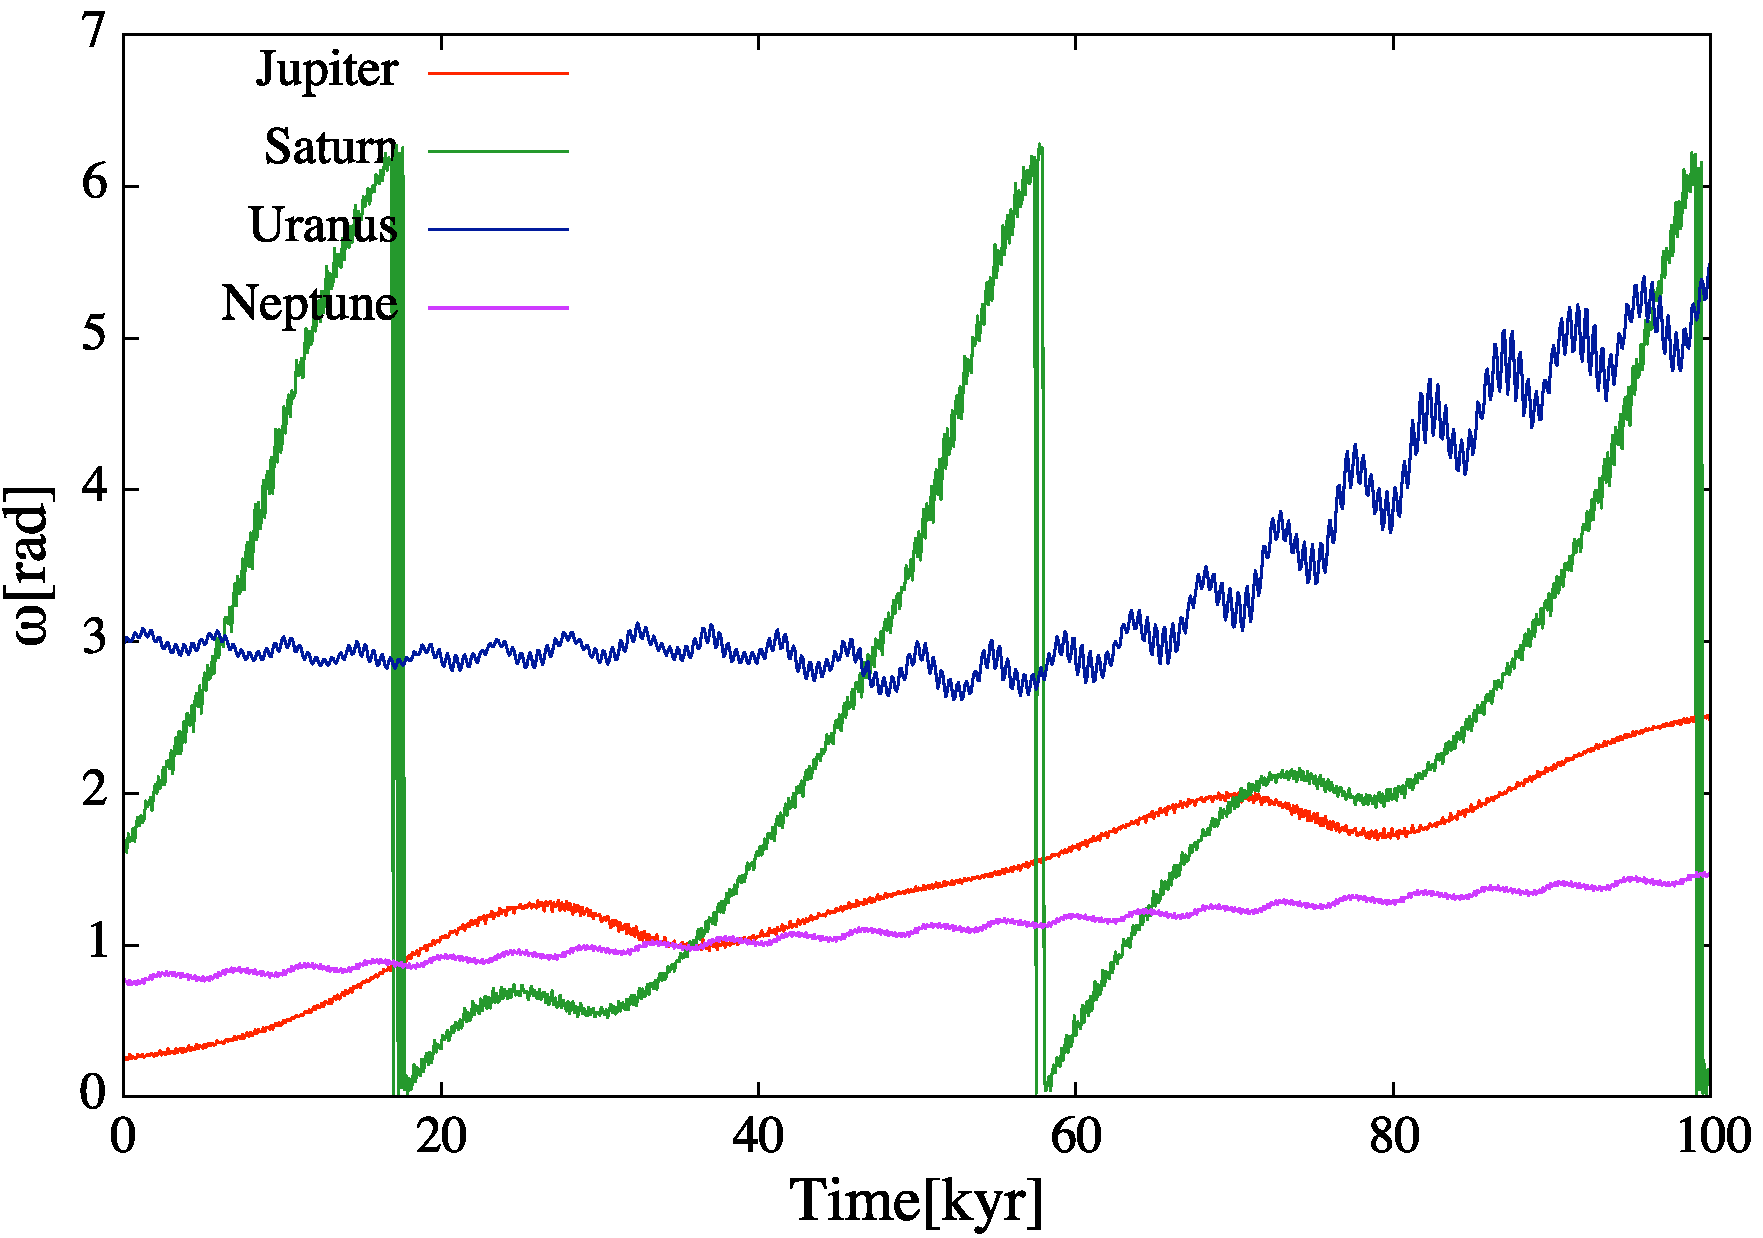
\includegraphics[width=7.6cm]{./image/Nomove_smallomega_100kyr.pdf}
\end{minipage} &
%右
\begin{minipage}[t]{0.45\hsize}
\centering
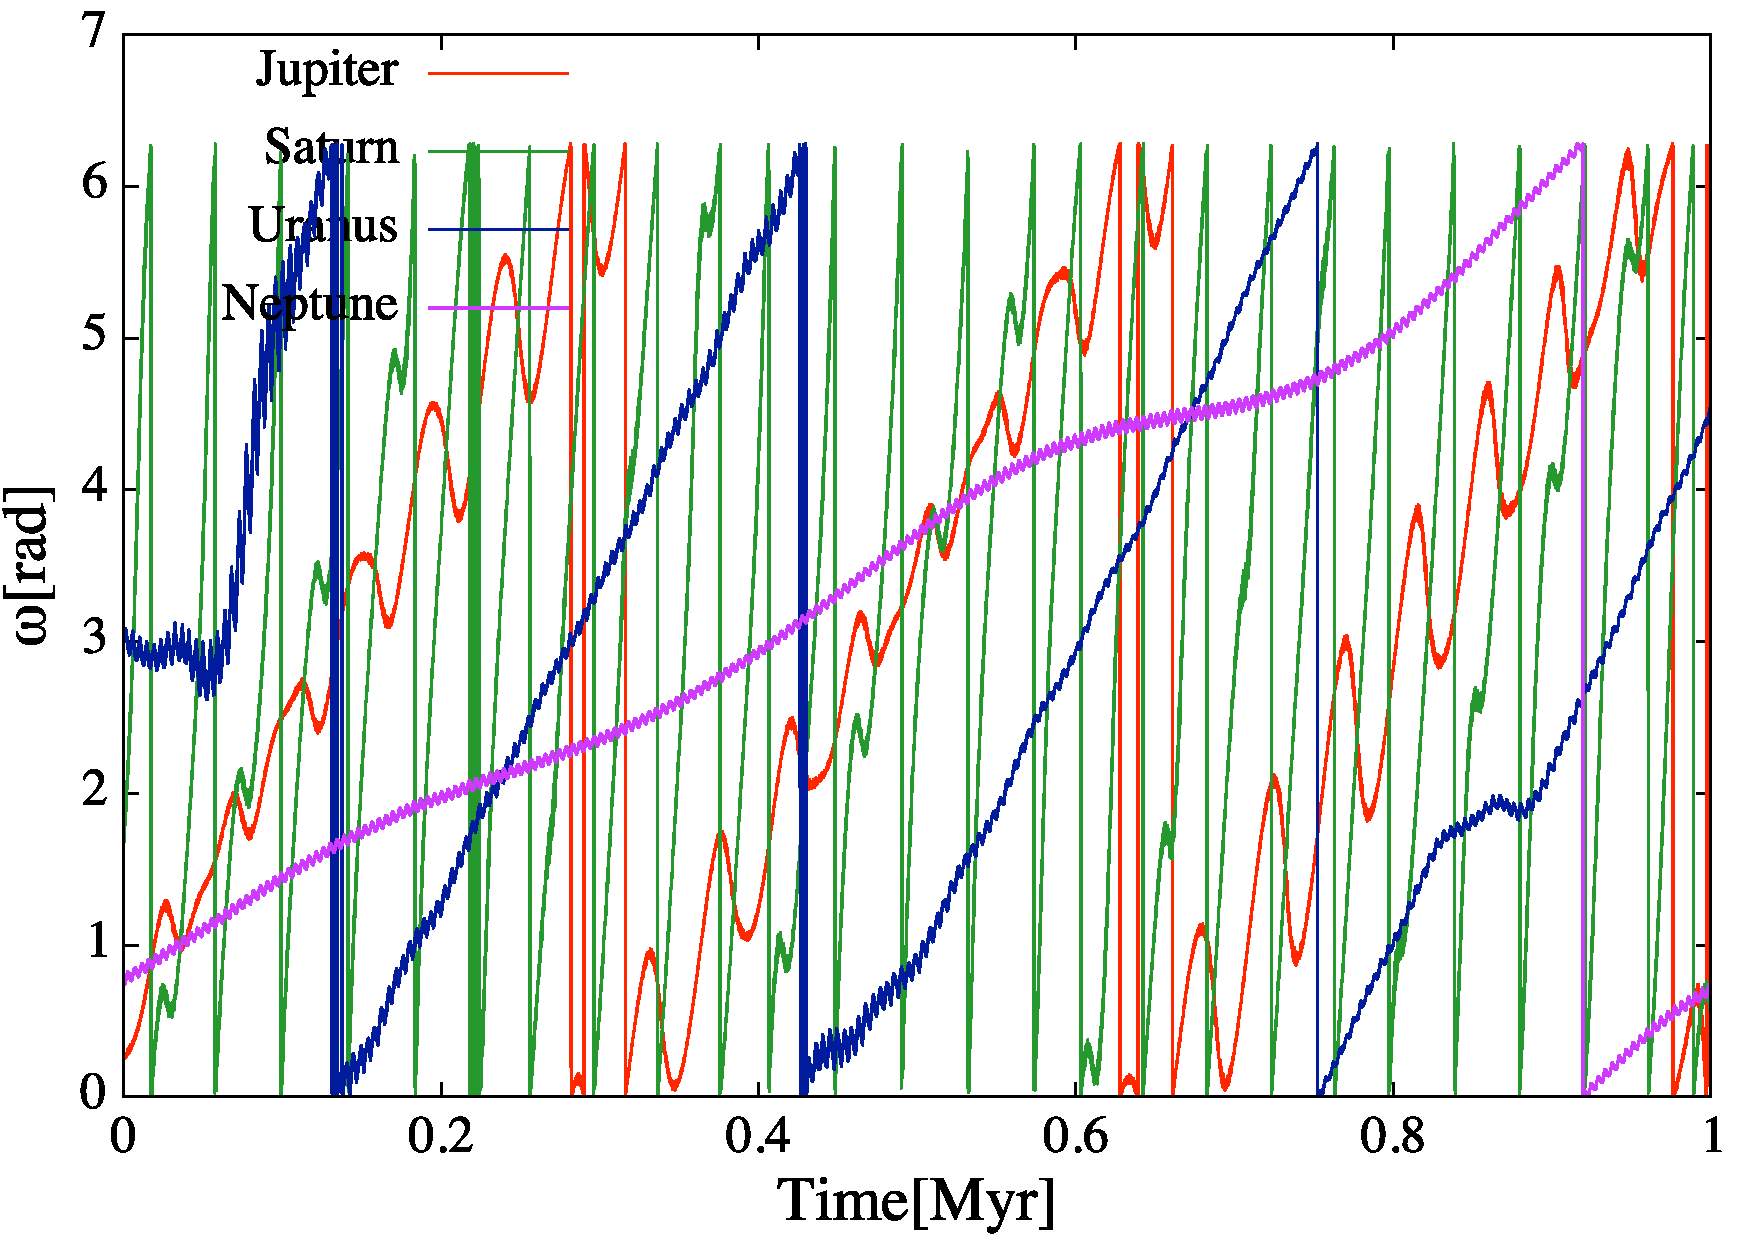
\includegraphics[width=7.6cm]{./image/Nomove_smallomega_1Myr.pdf}
\end{minipage}
%
\end{tabular}
\caption{\label{}}
\end{figure}


\subsubsection{移動をさせたときの巨大惑星の運動}

\begin{figure}[H]
\begin{tabular}{cc}
%左
\begin{minipage}[t]{0.45\hsize}
\centering
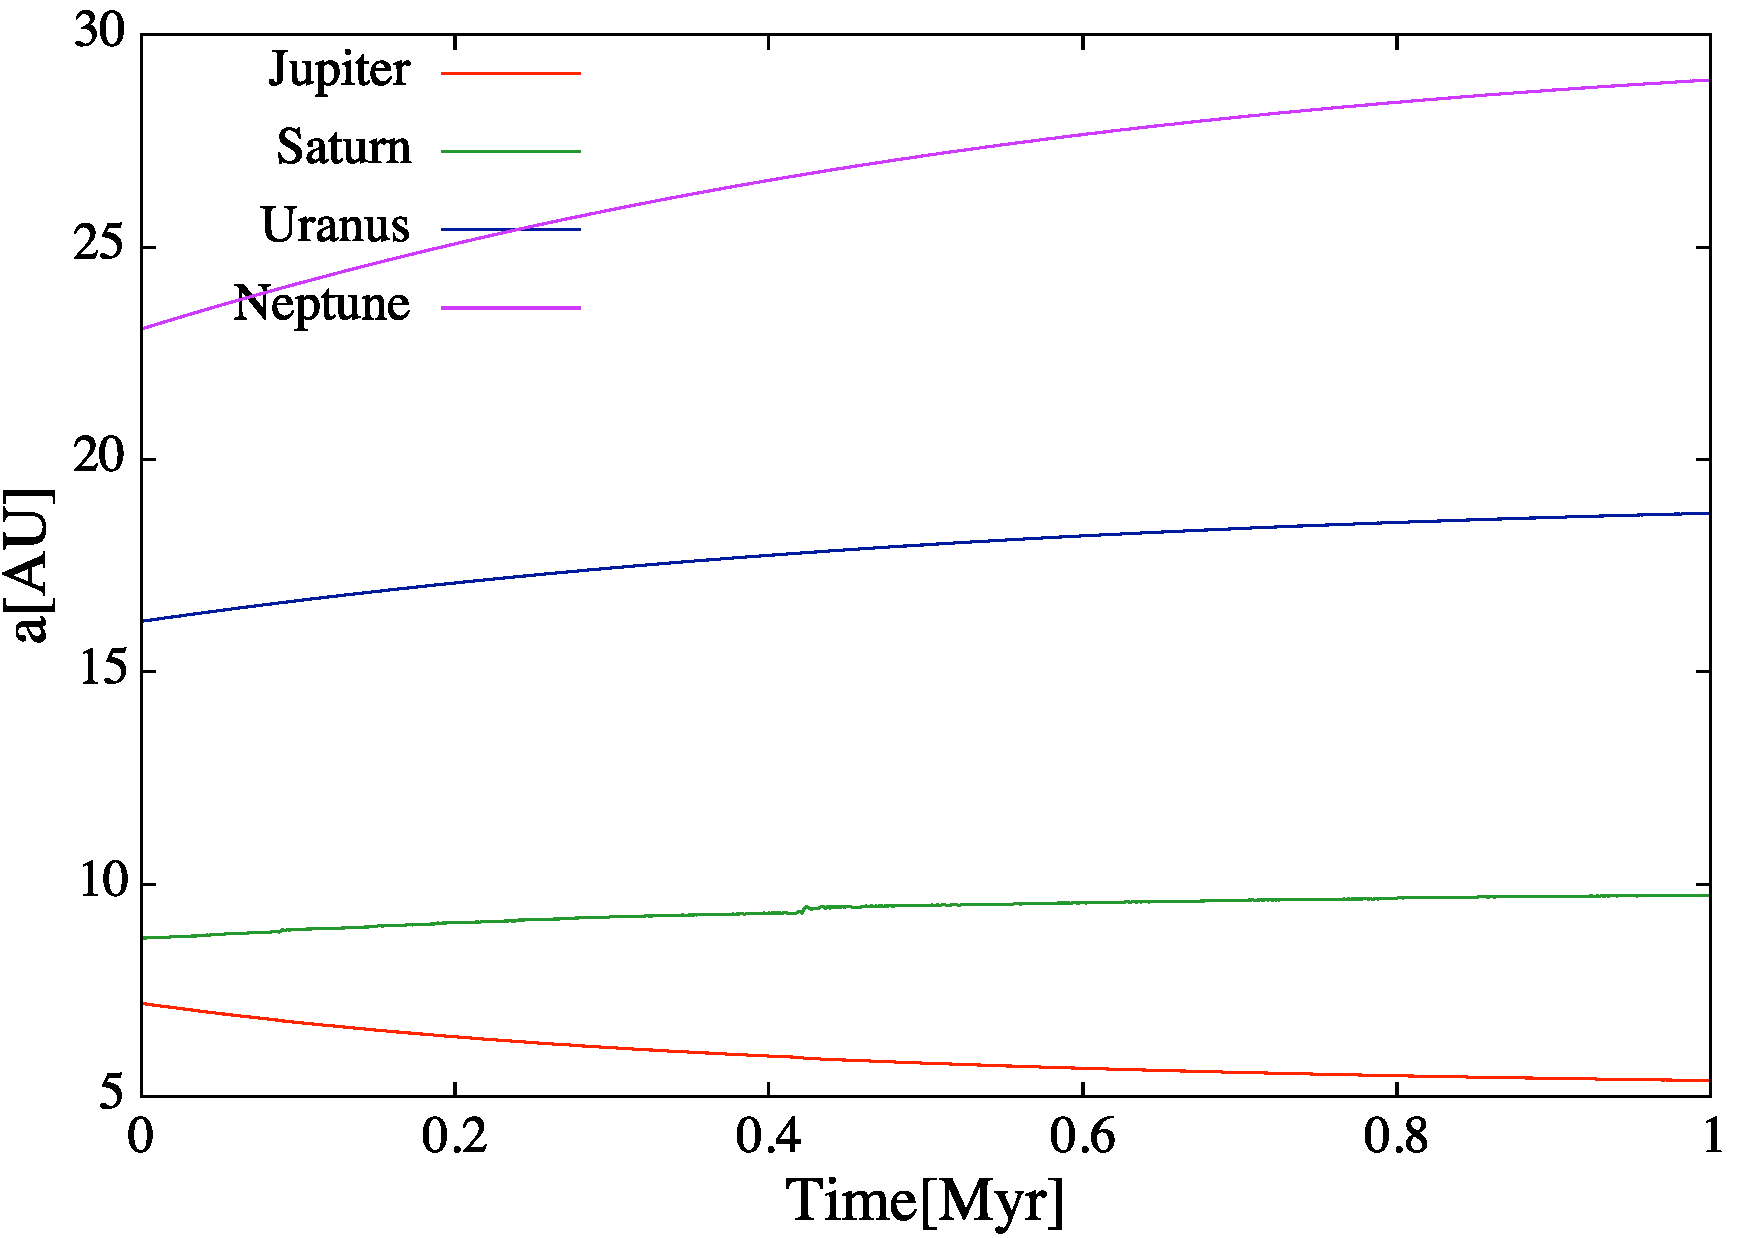
\includegraphics[width=7.6cm]{./image/move500kyr_a_1Myr.pdf}
\end{minipage} &
%右
\begin{minipage}[t]{0.45\hsize}
\centering
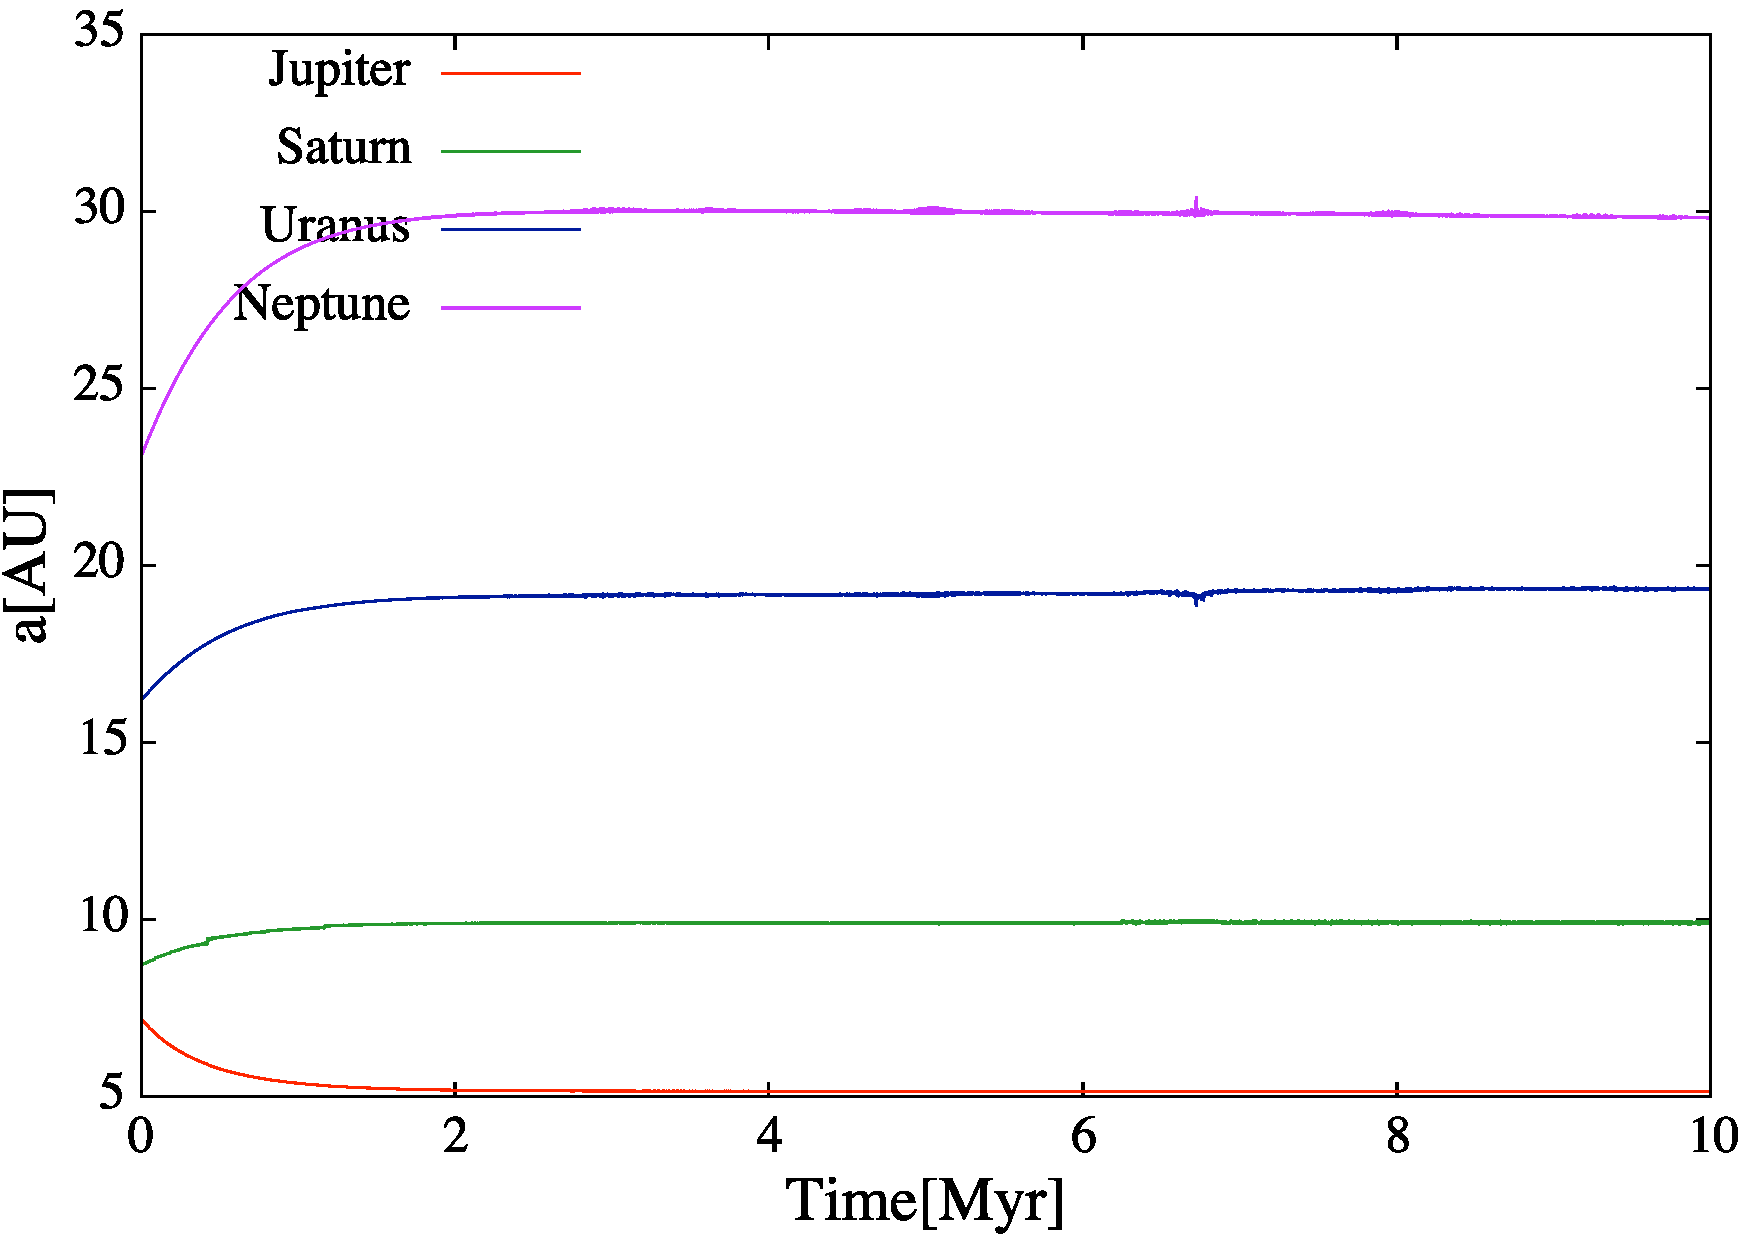
\includegraphics[width=7.6cm]{./image/move500kyr_a_10Myr.pdf}
\end{minipage}
%
\end{tabular}
\caption{\label{}}
\end{figure}


\begin{figure}[H]
\begin{tabular}{cc}
%左
\begin{minipage}[t]{0.45\hsize}
\centering
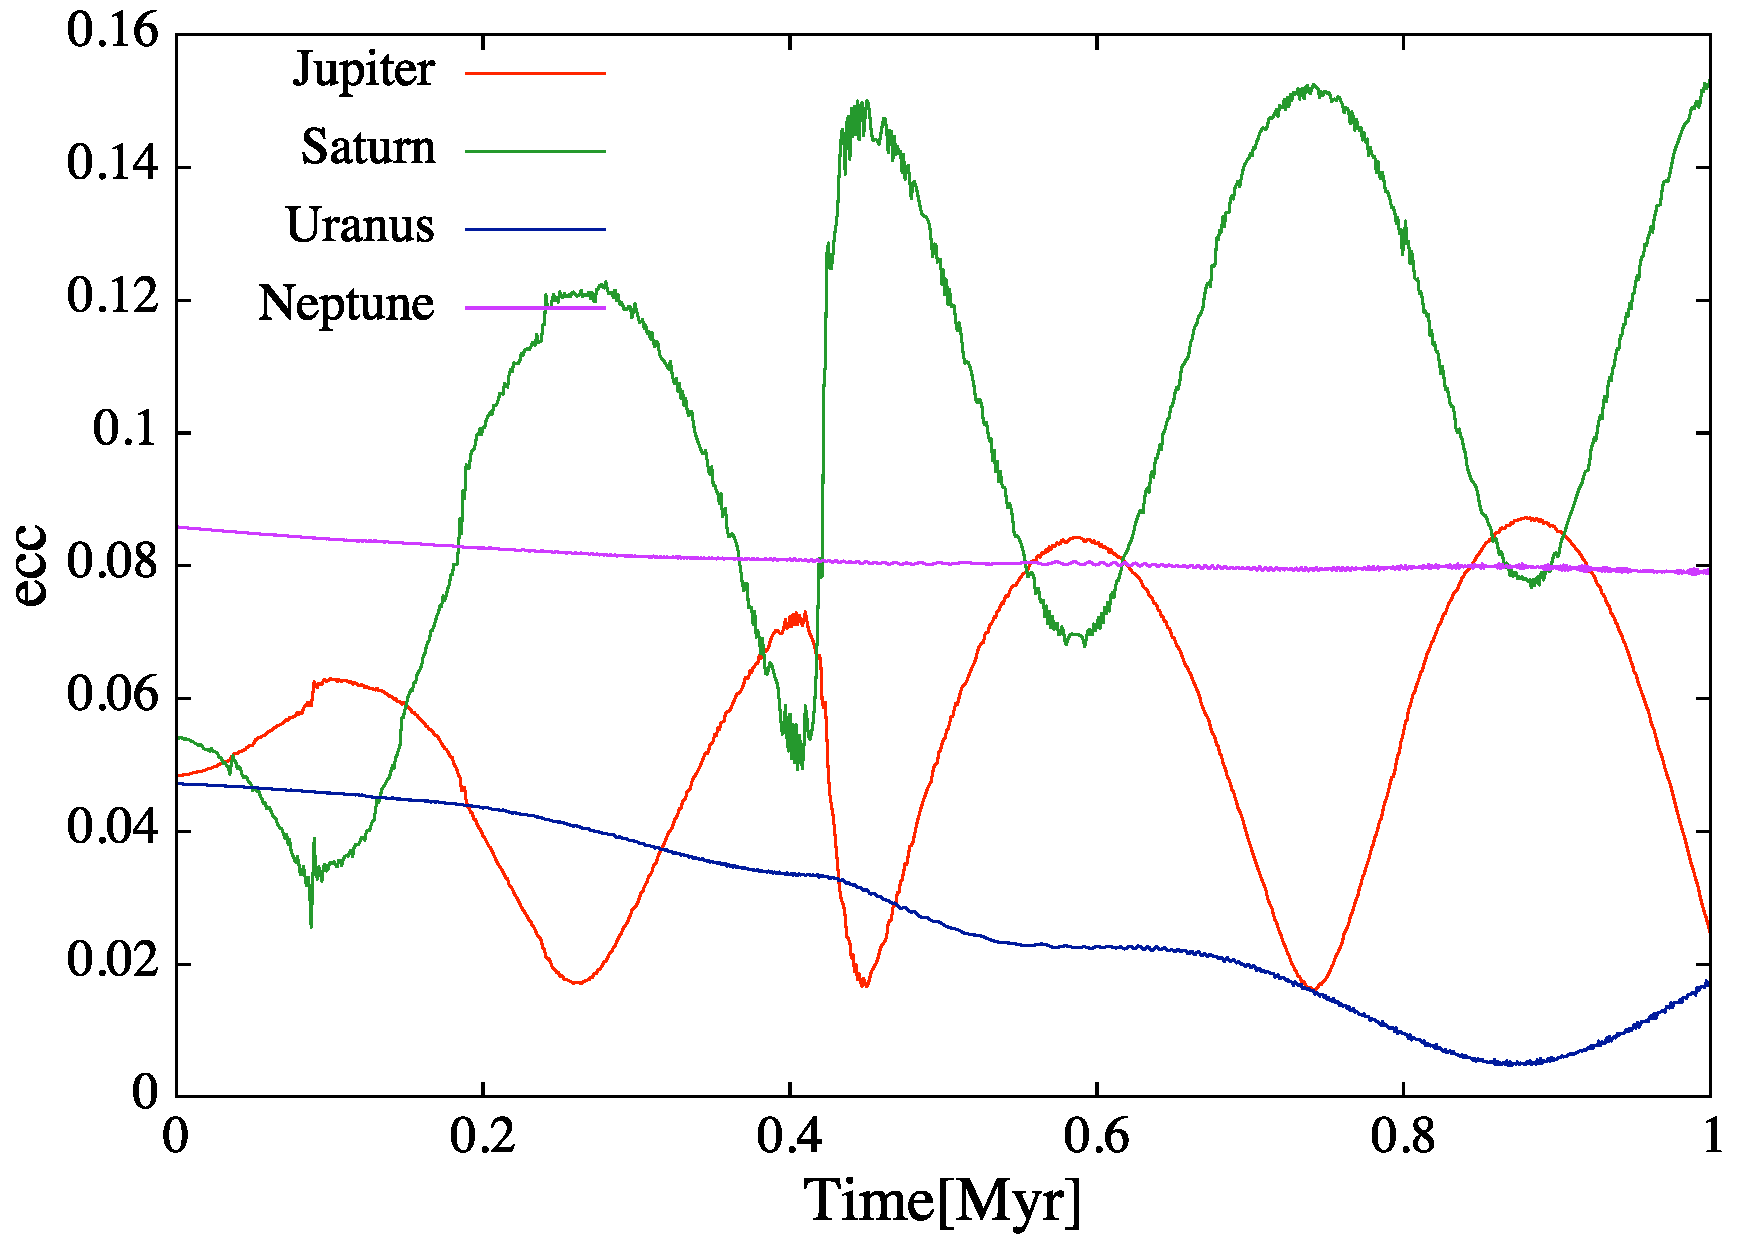
\includegraphics[width=7.6cm]{./image/move500kyr_ecc_1Myr.pdf}
\end{minipage} &
%右
\begin{minipage}[t]{0.45\hsize}
\centering
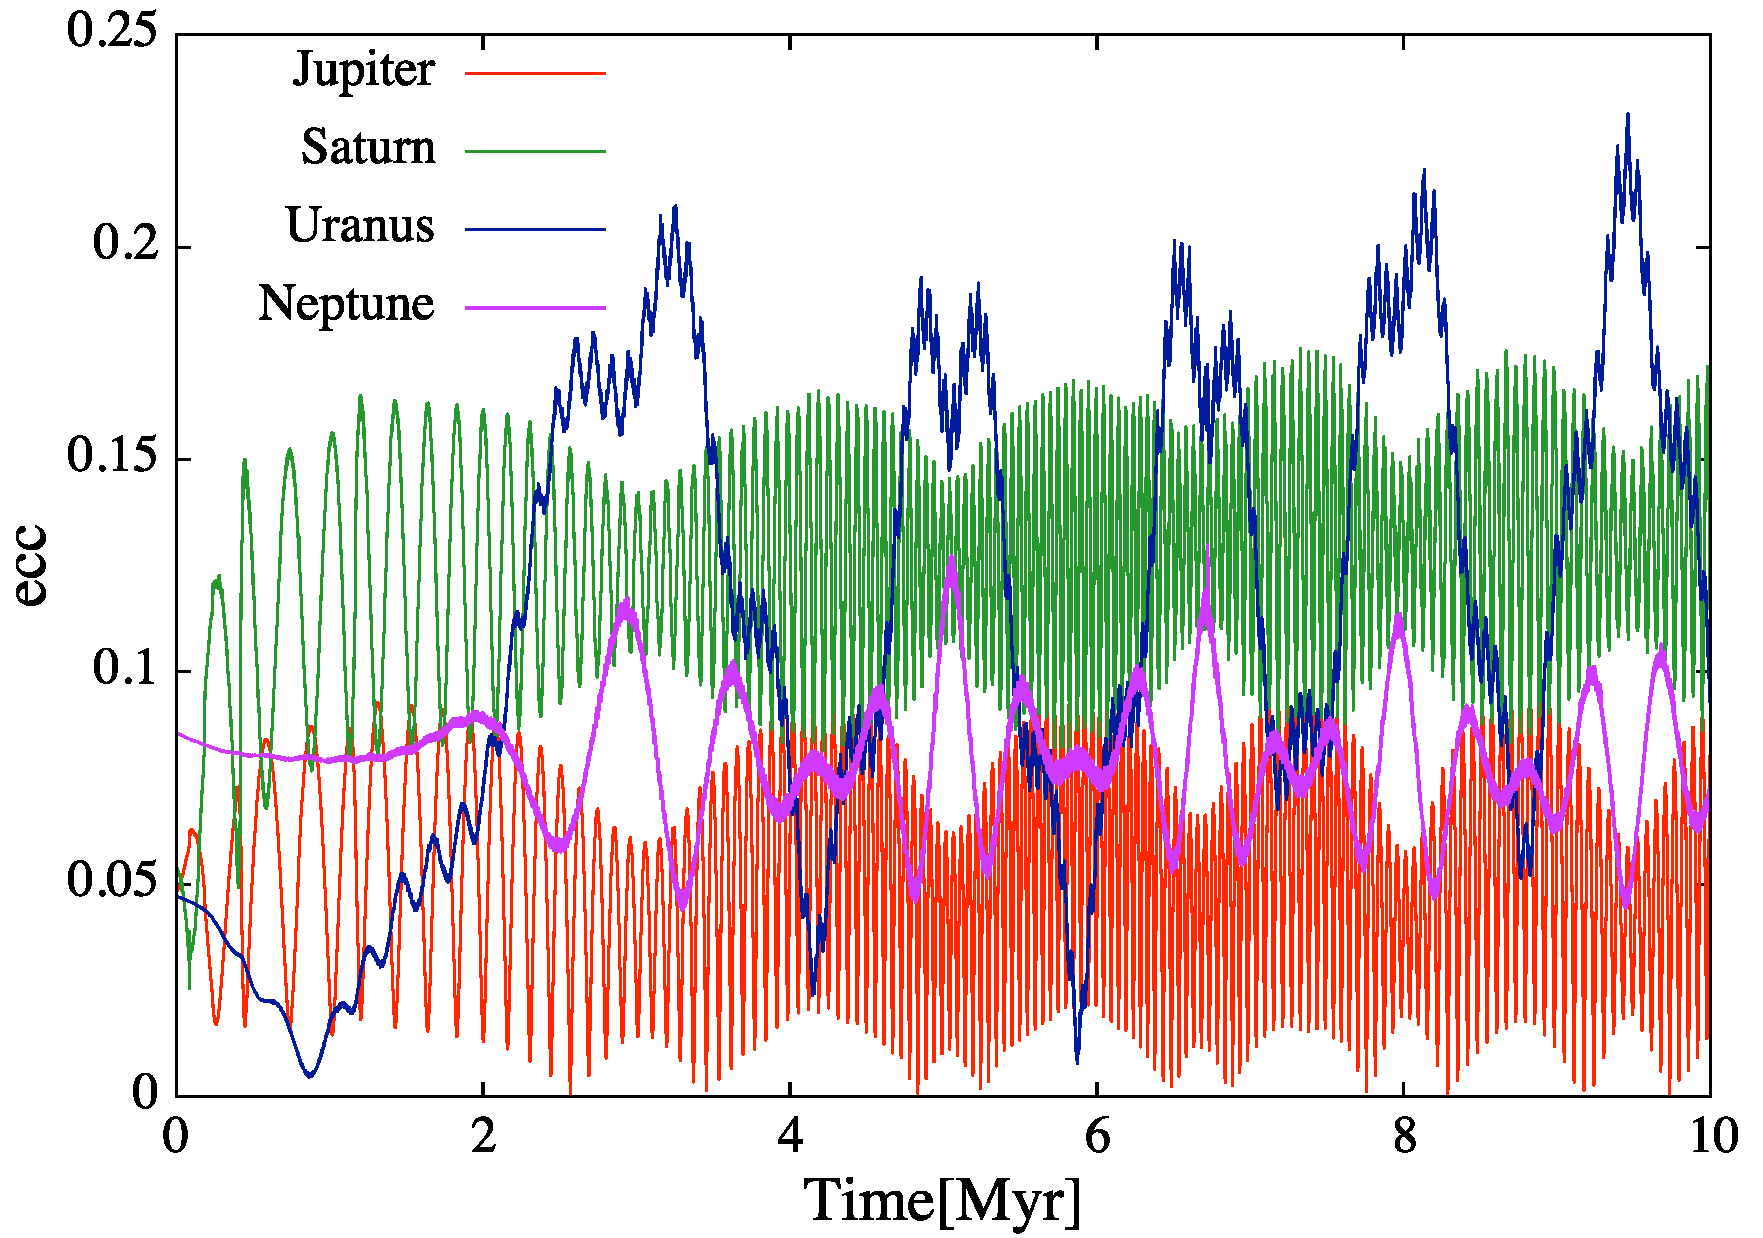
\includegraphics[width=7.6cm]{./image/move500kyr_ecc_10Myr.pdf}
\end{minipage}
%
\end{tabular}
\caption{\label{}}
\end{figure}


\begin{figure}[H]
\begin{tabular}{cc}
%左
\begin{minipage}[t]{0.45\hsize}
\centering
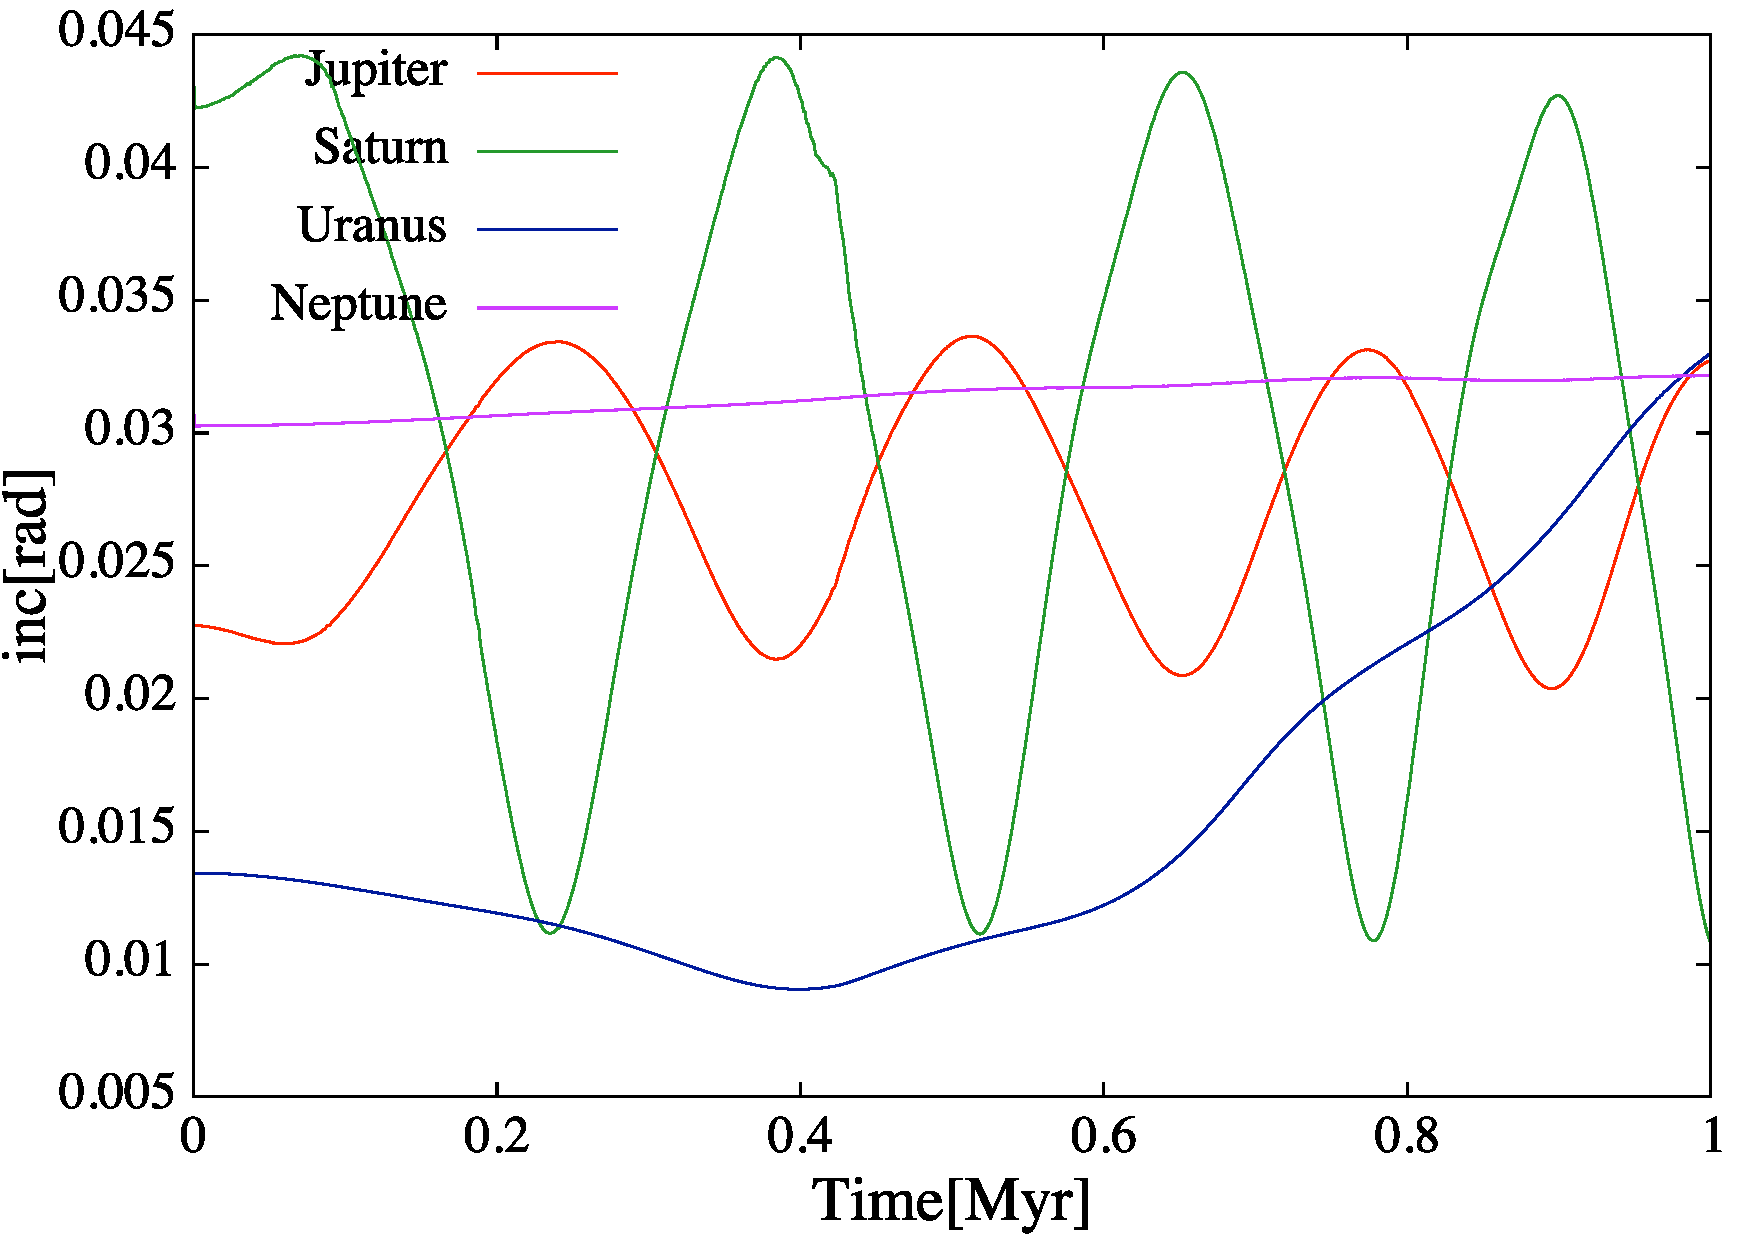
\includegraphics[width=7.6cm]{./image/move500kyr_inc_1Myr.pdf}
\end{minipage} &
%右
\begin{minipage}[t]{0.45\hsize}
\centering
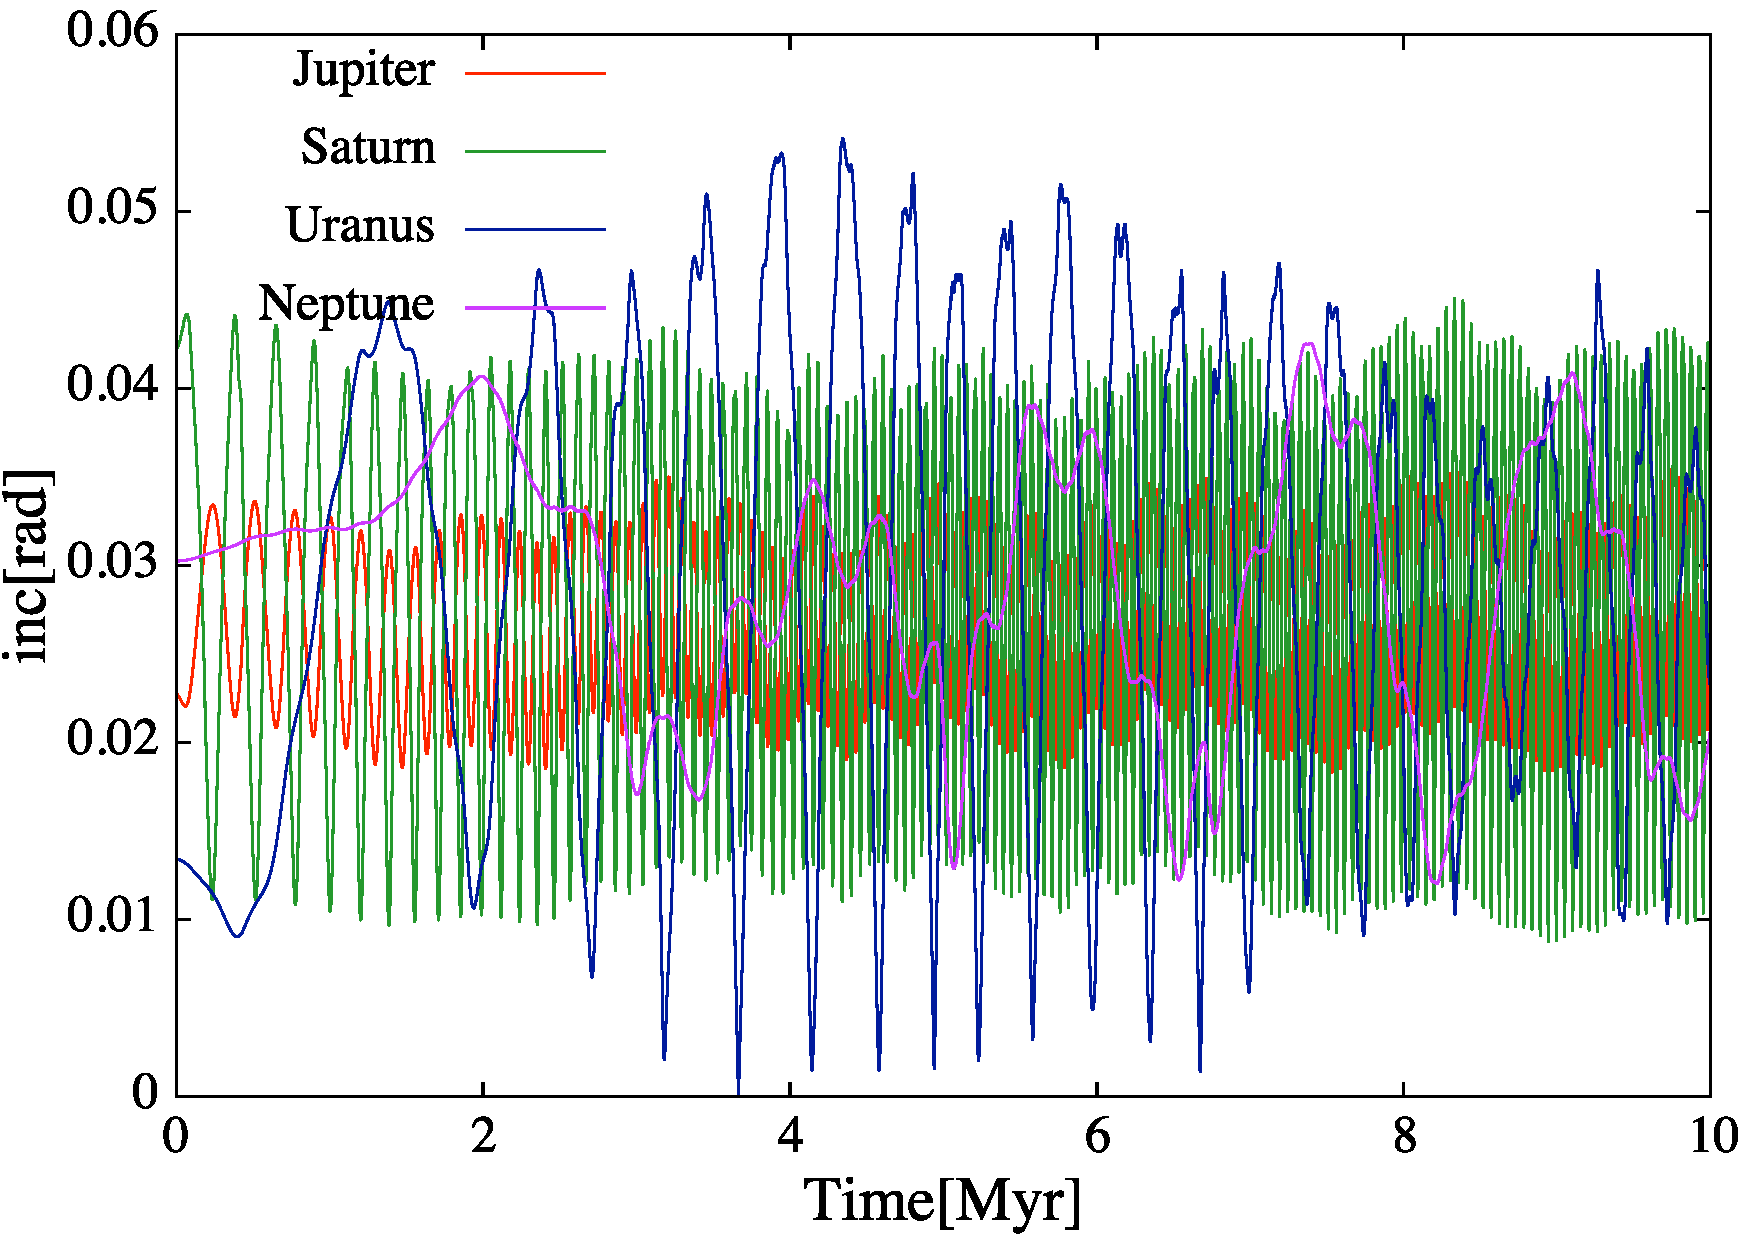
\includegraphics[width=7.6cm]{./image/move500kyr_inc_10Myr.pdf}
\end{minipage}
%
\end{tabular}
\caption{\label{}}
\end{figure}


\begin{figure}[H]
\begin{tabular}{cc}
%左
\begin{minipage}[t]{0.45\hsize}
\centering
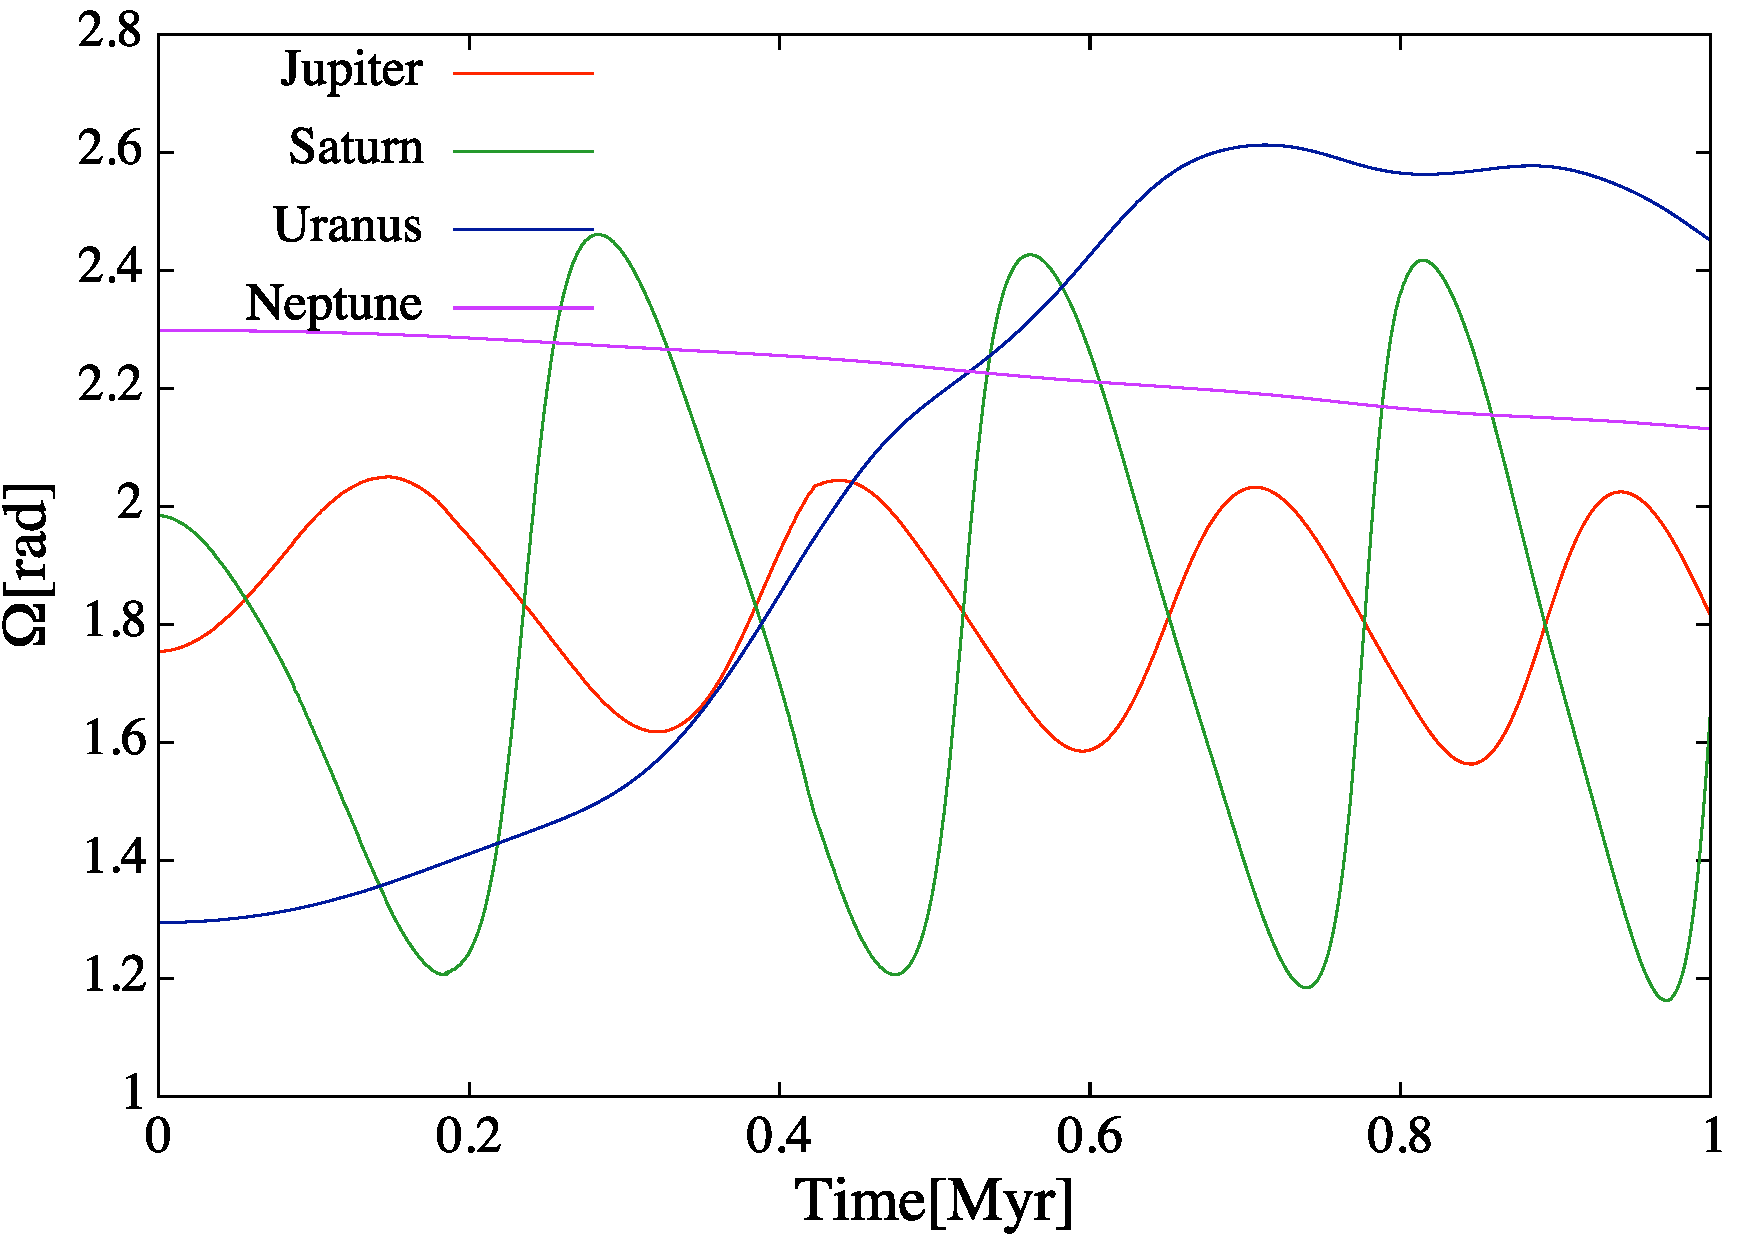
\includegraphics[width=7.6cm]{./image/move500kyr_capitalOMEGA_1Myr.pdf}
\end{minipage} &
%右
\begin{minipage}[t]{0.45\hsize}
\centering
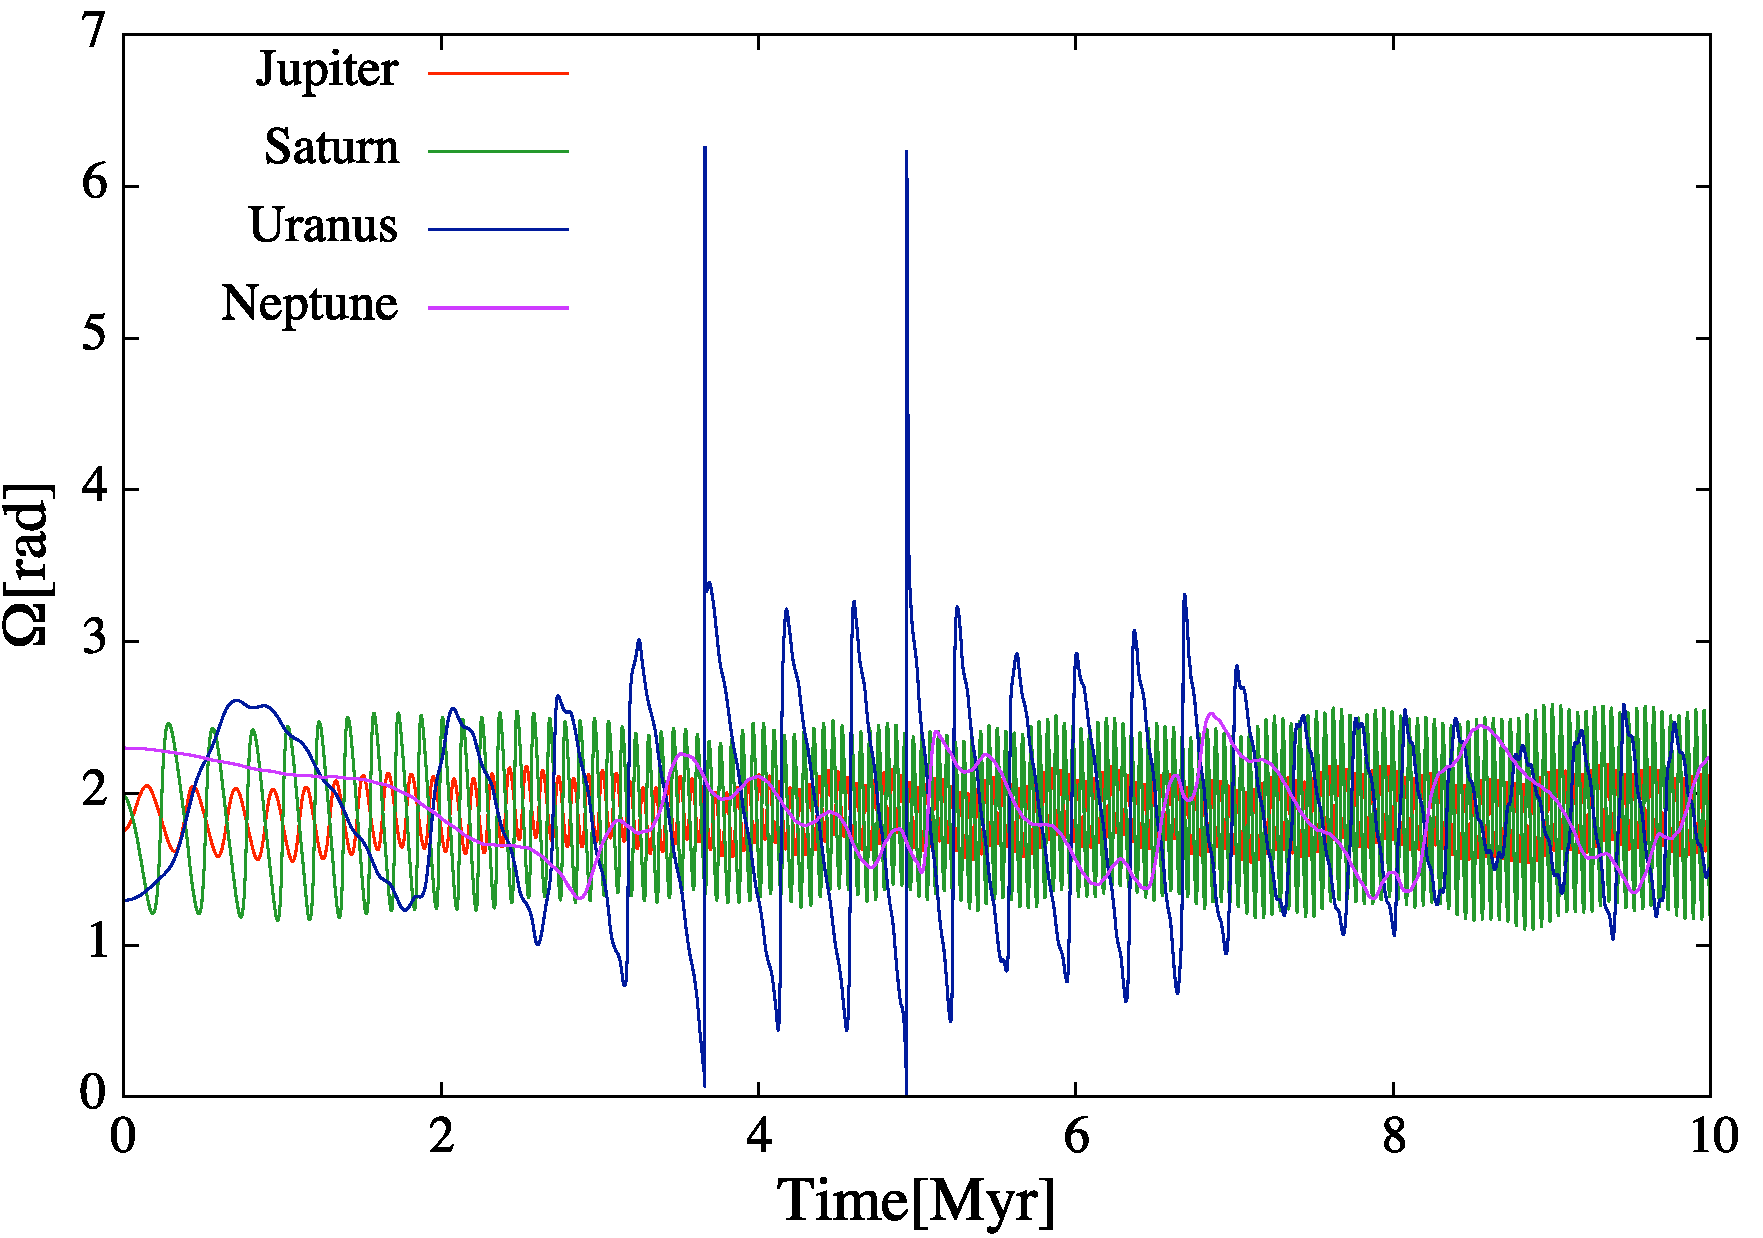
\includegraphics[width=7.6cm]{./image/move500kyr_capitalOMEGA_10Myr.pdf}
\end{minipage}
%
\end{tabular}
\caption{\label{}}
\end{figure}


\begin{figure}[H]
\begin{tabular}{cc}
%左
\begin{minipage}[t]{0.45\hsize}
\centering
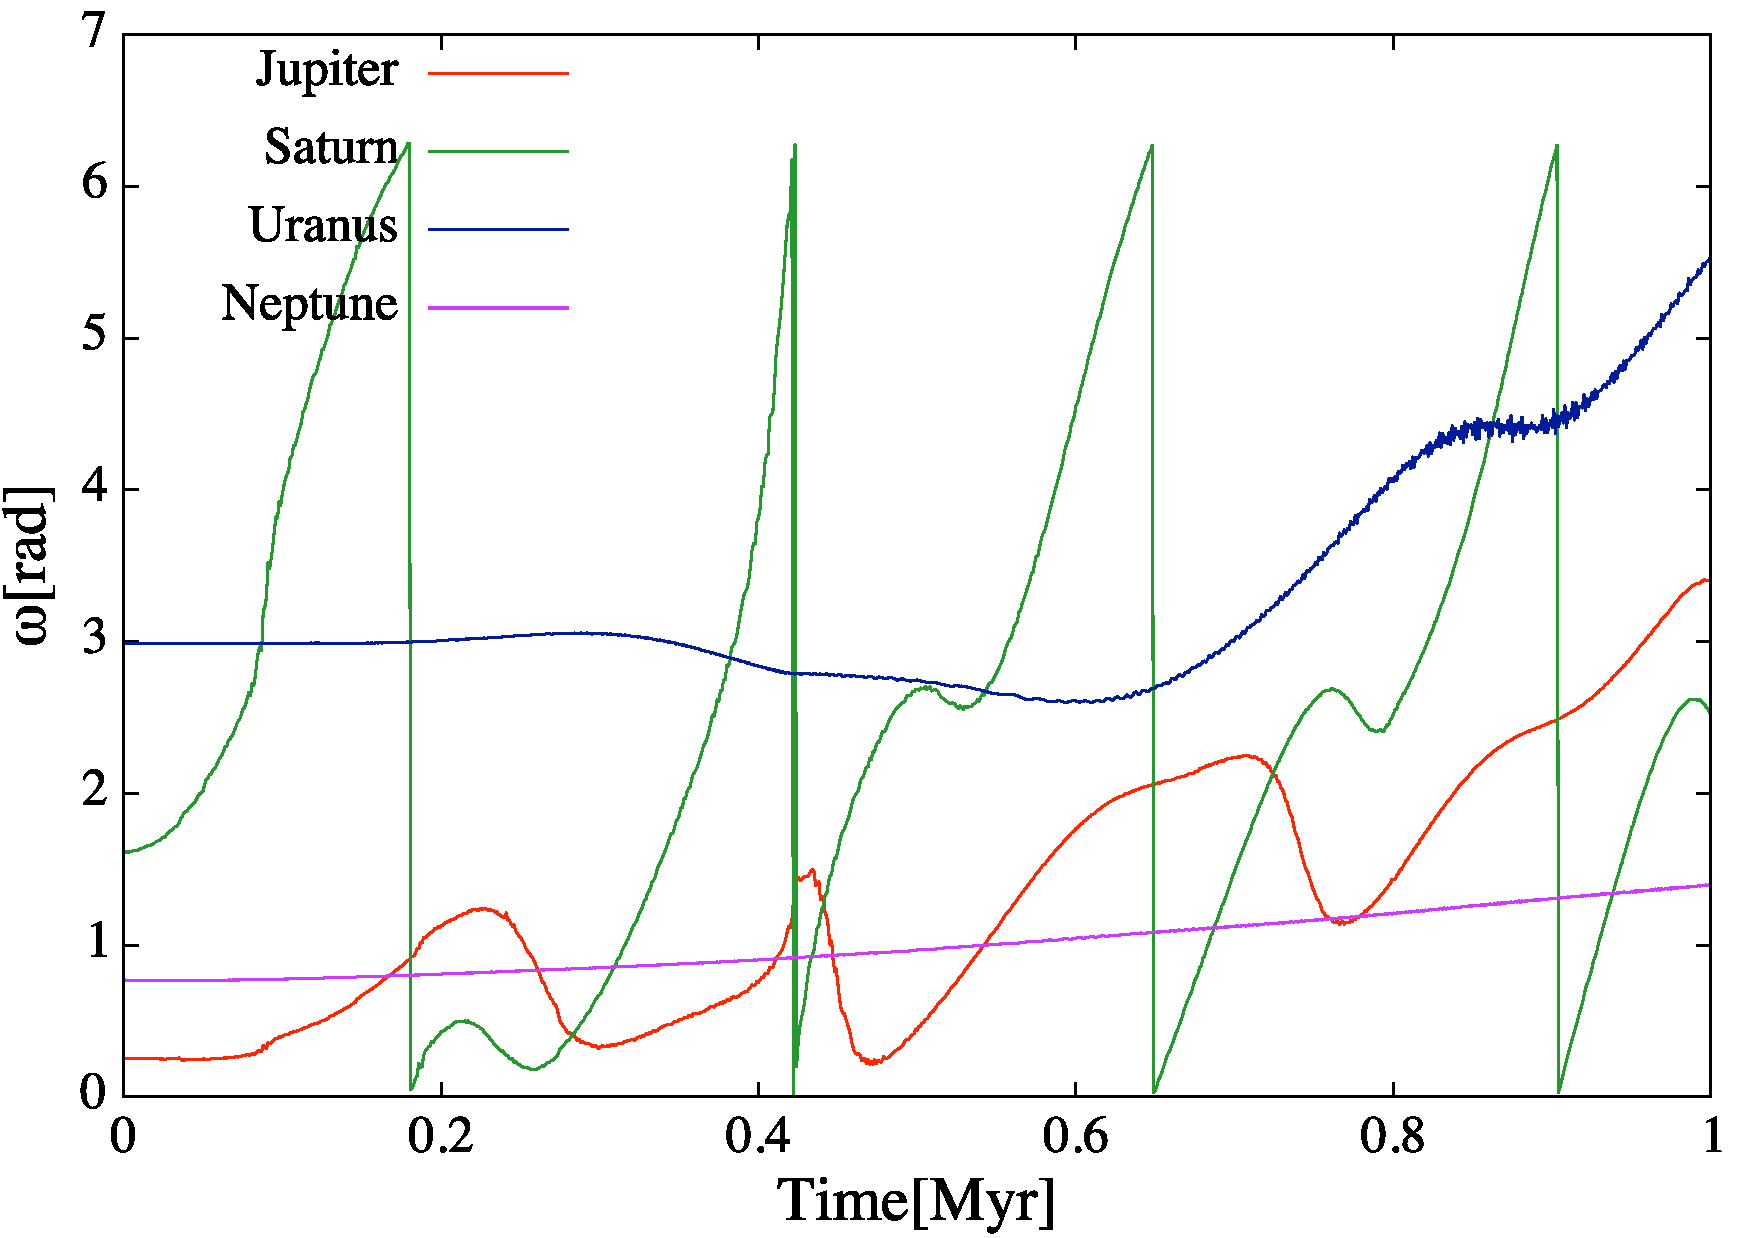
\includegraphics[width=7.6cm]{./image/move500kyr_smallomega_1Myr.pdf}
\end{minipage} &
%右
\begin{minipage}[t]{0.45\hsize}
\centering
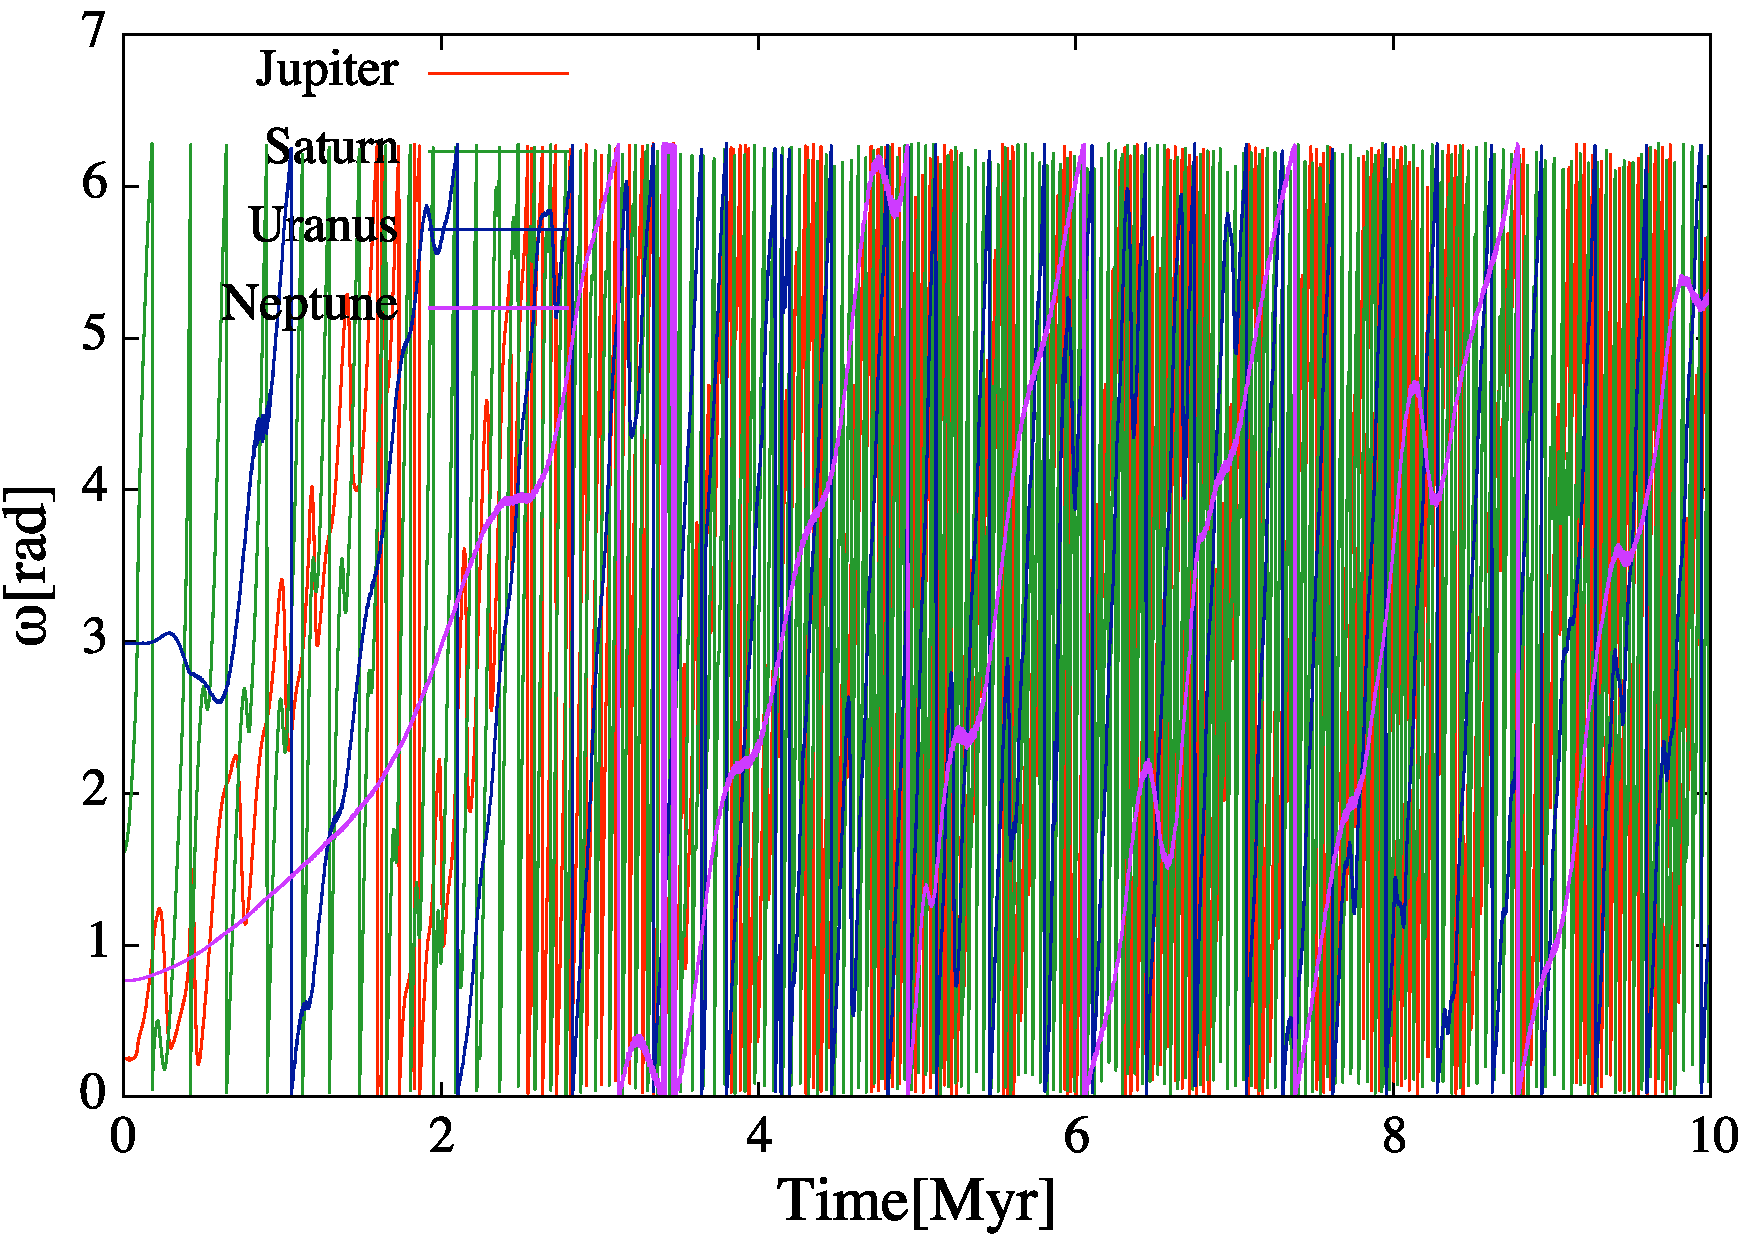
\includegraphics[width=7.6cm]{./image/move500kyr_smallomega_10Myr.pdf}
\end{minipage}
%
\end{tabular}
\caption{\label{}}
\end{figure}


\subsection{計算コードの見直し}
\begin{figure}[H]
\centering
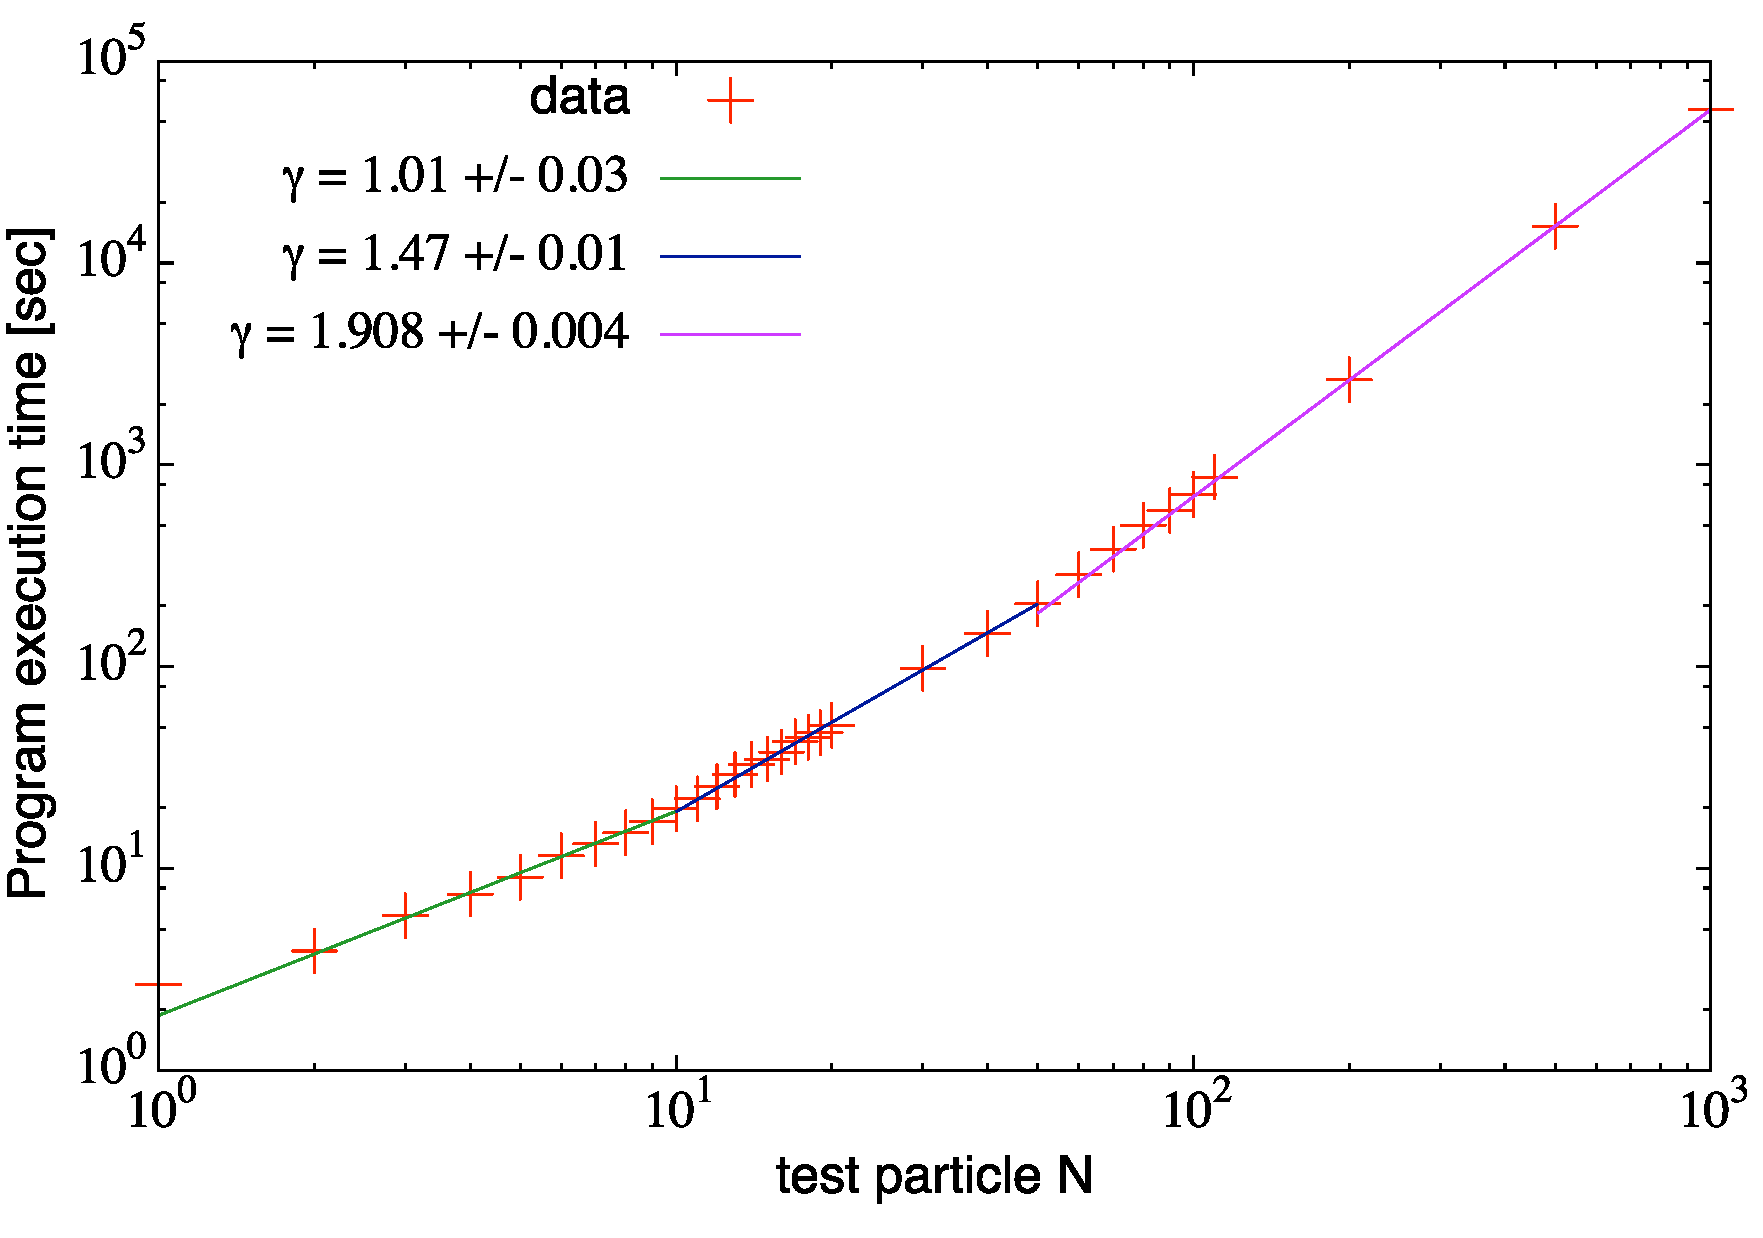
\includegraphics[width=10cm]{./image/Nbody_test.pdf}
\caption{\label{}}
\end{figure}

%%%%%%%%%%%%%%%%%%%%%%%%%%%%%%%%%%%%%%%%%%%%%
\begin{thebibliography}{9}
  \bibitem{1} Carl D. Murray and Stanley F. Dermott 1999, Solar System Dynamics
  \bibitem{2} 富坂幸治, 花輪知幸, 牧野淳一郎 2007, シリーズ現代の天文学 14 シミュレーション天文学
  \bibitem{3} 木下宙, 天体と軌道の力学
\end{thebibliography}
%%%%%%%%%%%%%%%%%%%%%%%%%%%%%%%%%%%%%%%%%%%%%

\end{document}